\documentclass[12pt,a4paper]{report}
\usepackage[top = 1.6cm, left = 2.7cm, right = 2.7cm ]{geometry}
\usepackage{setspace}
\usepackage[utf8]{inputenc}
\usepackage[francais]{babel}
\usepackage{float}
\usepackage[T1]{fontenc}
\usepackage{amsmath}
\usepackage{amsthm}
\usepackage{amsfonts}
\usepackage{amssymb}
\usepackage{graphicx}
\usepackage{hyperref}
\usepackage{amsthm,thmtools}
\usepackage{cite}
\usepackage{bbm}
\usepackage{caption}
\usepackage{xcolor}
\usepackage{framed}
\usepackage{rotating}
\usepackage[noend]{algorithmic}
\usepackage{algorithm}
\usepackage{minted}
\usepackage{cprotect}
\usepackage{caption}
\usepackage{fancyvrb}
\usepackage{afterpage}
%\usepackage[noend]{algcompatible}
\colorlet{shadecolor}{lightgray!25}

%% ALGORITHME

\floatname{algorithm}{Algorithme}
\renewcommand{\algorithmicrequire}{\textbf{Entrée :}}
\renewcommand{\algorithmicensure}{\textbf{Sortie :}}
\renewcommand{\algorithmicif}{\textbf{si}}
\renewcommand{\algorithmicthen}{\textbf{alors}}
\renewcommand{\algorithmicelse}{\textbf{sinon}}
\renewcommand{\algorithmicelsif}{\textbf{sinon si}}
\renewcommand{\algorithmicwhile}{\textbf{tant que}}
\renewcommand{\algorithmicdo}{\textbf{faire}}
\renewcommand{\algorithmicend}{\textbf{fin}}
\renewcommand{\algorithmicreturn}{\textbf{retourner}}
\renewcommand{\algorithmicfor}{\textbf{pour}}
\renewcommand{\algorithmicforall}{\textbf{pour tout}}

%% Theorem Styles %%

\theoremstyle{definition}%{3pt}{3pt}{\slshape}{}{\bfseries}{.}{.5em}{}
\newtheorem{definition}{Définition}[chapter]
\newtheorem{theorem}{Théorème}[chapter]
\newtheorem{lemma}{Lemme}[chapter]
\newtheorem*{notation}{Notation}
\newtheorem*{notations}{Notations}
\newtheorem{propriete}{Propriété}[chapter]
\newtheorem*{proprietes}{Propriétés}
\newtheorem{proposition}{Proposition}[chapter]
\newtheorem{corollaire}{Corollaire}[chapter]
\theoremstyle{remark}
\newtheorem{example}{Exemple}[chapter]
\newtheorem{remark}{Remarque}[chapter]

%%Definition by chapter%%

\usepackage{etoolbox}
\makeatletter
\patchcmd\thmtlo@chaptervspacehack
{\addtocontents{loe}{\protect\addvspace{10\p@}}}
{\addtocontents{loe}{\protect\thmlopatch@endchapter\protect\thmlopatch@chapter{\thechapter}}}
{}{}
\AtEndDocument{\addtocontents{loe}{\protect\thmlopatch@endchapter}}
\long\def\thmlopatch@chapter#1#2\thmlopatch@endchapter{%
	\setbox\z@=\vbox{#2}%
	\ifdim\ht\z@>\z@
	\hbox{\bfseries\chaptername\ #1}\nobreak
	#2
	\addvspace{10\p@}
	\fi
}
\def\thmlopatch@endchapter{}

\makeatother
\renewcommand{\thmtformatoptarg}[1]{ -- #1}

%% Commandes persos %%
\newcommand\bbone{\ensuremath{\mathbbm{1}}}
\newcommand{\eg}{e.g., }
\newcommand{\ssi}{ssi }
\newcommand{\ie}{i.e., }
\newcommand{\cf}{cf. }
\newcommand{\pr}{\mathbb{P}}
\renewcommand{\listtheoremname}{Définitions et théorèmes}

\setstretch{1,1}
\let\labelitemi\labelitemii


\begin{document}
\begin{titlepage}

	\newcommand{\HRule}{\rule{\linewidth}{0.5mm}} % Defines a new command for the horizontal lines, change thickness here

	\center % Center everything on the page
	%----------------------------------------------------------------------------------------
	%	HEADING SECTIONS
	%----------------------------------------------------------------------------------------


	\begin{center}
	\includegraphics[height=2cm]{logos/UMONS_FS.pdf}
	\hspace{5cm}
	\includegraphics[height=1.7cm]{logos/UMONS+txt}
	\\[1em]
	\vspace{1cm}
	\end{center}
	\textsc{\large Service d'informatique théorique }\\[0.5cm] % Major heading such as course name

	%\vspace{1cm}
	%----------------------------------------------------------------------------------------
	%	TITLE SECTION
	%----------------------------------------------------------------------------------------

	\vspace{0.5cm}
	\HRule \\[0.4cm]
	{\huge \bfseries \centering \quad Plus court chemin stochastique dans\newline \newline les Processus Décisionnels  de Markov}\\[0.4cm] % Title of your document
	\HRule \\[1cm]
	%{\large Projet de Master 1}

	%----------------------------------------------------------------------------------------
	%	AUTHOR SECTION//
	%----------------------------------------------------------------------------------------
	\vspace{2cm}
	\begin{minipage}{0.4\textwidth}
		\begin{flushleft} \large
			\emph{Auteur :} \\Florent Delgrange
		\end{flushleft}
	\end{minipage}
	~
	\begin{minipage}{0.4\textwidth}
		\begin{flushright} \large
			\quad \\
			\emph{Directeurs:}\\ \quad Véronique Bruyère \\ \quad Mickael Randour\\	\vspace*{0.5cm}
			%\emph{Rapporteur:}\\
			%Quentin Hautem
		\end{flushright}

	\end{minipage}\\[5cm]

	% If you don't want a supervisor, uncomment the two lines below and remove the section above
	%\Large \emph{Author:}\\
	%John \textsc{Smith}\\[3cm] % Your name

	%----------------------------------------------------------------------------------------
	%	DATE SECTION
	%----------------------------------------------------------------------------------------
	\vspace{3.7cm}
	%{\large \today}\\[3cm] % Date, change the \today to a set date if you want to be precise
	\begin{center}
			Ann\'ee acad\'emique 2016-2017
	\end{center}

	%----------------------------------------------------------------------------------------
	%	LOGO SECTION
	%----------------------------------------------------------------------------------------
	%----------------------------------------------------------------------------------------

	\vfill % Fill the rest of the page with whitespace

\end{titlepage}

\pagenumbering{gobble}
\shipout\null
\begin{flushright}
{\Large \textbf{Remerciements}} \\
\end{flushright}

\begin{flushright}
Je remercie toutes les personnes qui ont contribué à ce projet et qui m'ont soutenu durant sa réalisation, tout
particulièrement Véronique Bruyère et Mickael Randour pour leurs précieux
conseils, mais aussi Carolane Gerbehaye pour son appui.
\end{flushright}
\thispagestyle{empty}

\afterpage{\null\newpage}

\tableofcontents
\listoftheorems[ignoreall,show={definition,theorem}]

\afterpage{\null\newpage}

\chapter*{Introduction}
\pagenumbering{arabic}
\setcounter{page}{9}
La résolution du problème du plus court chemin dans un graphe possède une quantité indénombrable d'applications, comme par exemple
l'optimisation des réseaux de télécommunications ou la détermination du chemin le
plus court entre deux villes via un réseau routier.
Mais qu'en est-il lorsque l'environnement du problème que l'on étudie est
stochastique et sujet à des phénomènes aléatoires divers ? En pratique,
très peu de situations se déroulent dans un environnement parfait et cela est
rare de pouvoir affirmer l'exactitude du contexte du problème que l'on traite.
Les \textit{processus décisionnels de Markov} permettent de modéliser ces situations
évoluant dans un milieu stochastique et dans
lesquelles des prises de décisions sont requises. \\

Les processus décisionnels de Markov sont des automates probabilistes dans
lesquels une prise de décision est requise à chaque étape. Chaque décision a un
coût et, lorsque le système est en un état, la prise de décision
entraine un comportement probabiliste du système, qui
évolue ensuite dans l'état suivant.
On va donc définir des \textit{stratégies}
qui détermineront, à chaque étape, la décision à prendre afin que le système évolue dans l'état suivant. Par le fait que l'environnement du système est probabiliste, la stratégie ne peut assurer au système d'évoluer vers un ou plusieurs états avec un chemin de coût fixe et ne peut donc pas résoudre le problème du plus court chemin à proprement parler. On parle donc de \textit{plus
court chemin stochastique}. Ce problème peut être abordé par différentes
approches. Dans ce document, on va définir des stratégies qui vont maximiser
\textit{l'espérance de la longueur du plus court chemin} et \textit{la probabilité d'accessibilité avec des chemins de taille inférieure à un seuil}.
De cette façon, lorsqu'on souhaitera voyager entre deux villes via un réseau
routier, de par le caractère stochastique du voyage, il sera plus intéressant
d'étudier ces problèmes de plus court chemin stochastique dans le processus
décisionnel de Markov qui lui est associé. \\
%qui modélise le problème. \par

Le but final de ce travail est d'implémenter les processus décisionnels de Markov, le problème d'accessibilité et
les deux problèmes de plus court chemin stochastique qui leur sont associés.
Pour ce faire, on va tout d'abord définir ce qu'est une
probabilité, comment la mesurer et dans quelles conditions. Ensuite, nous allons étudier
des systèmes qui modélisent des phénomènes aléatoires (i.e., les \textit{chaînes de Markov}) qui seront indispensables
pour mesurer la probabilité des \textit{chemins} d'un processus décisionnel de Markov.
En effet, on va voir que le non-déterminisme lié à la prise de décision
ne permet pas de mesurer la probabilité des chemins des processus
décisionnels de Markov sans les notions de stratégies et de chaîne de Markov.
C'est ce qui va nous amener à traiter les problèmes \textit{d'accessibilité, d'espérance du coût de l'accessibilité} ainsi que celui de \textit{l'accessibilité limitée par un coût}
dans une chaîne de Markov.
Finalement, cela nous permettra d'étudier les processus décisionnels de Markov
et les stratégies qui vont résoudre les problèmes \textit{d'accessibilité,
d'espérance du plus court chemin stochastique} ainsi que celui des \textit{plus courts
chemins stochastiques de taille limitée}.

\chapter{Introduction aux probabilités}
Les processus décisionnels de Markov sont des systèmes qui modélisent des situations aléatoires enrichis par des probabilités. Avant de définir formellement de tels modèles, il est utile d'introduire brièvement quelques notions de probabilités qui seront indispensables à la compréhension de la suite du document.

\begin{definition}[\textbf{$\sigma$-algèbre}]
	Une $\sigma$-algèbre est une paire $(\Omega, \sigma)$ où $\Omega$ est un ensemble non-vide et $\sigma \subseteq \mathcal{P}(\Omega)$ qui respecte les $3$ conditions suivantes :
	\begin{enumerate}
		\item $\varnothing \in \sigma$
		\item Si $E \in \sigma$, alors $\overline{E} = \Omega \setminus E$ et $\overline{E} \in \sigma$
		\item Si $E_1, E_2, \dots \in \sigma$, alors $\bigcup_{n \geq 1} E_n \in \sigma$
	\end{enumerate}
	Les éléments de $\Omega$ sont appelés \textit{résultats} et les éléments de $\sigma$ sont appelés \textit{évènements}.
\end{definition}

\begin{remark} \label{probaremark}
	Ces conditions sur la $\sigma$-algèbre mènent au fait que
	\begin{itemize}
		\renewcommand{\labelitemi}{\tiny$\bullet$}
		\item
	$\Omega \in \sigma$. En effet, on a que $\Omega$ est non-vide par définition et $\varnothing \in \sigma$. Donc, $\overline{\varnothing} = \Omega \setminus \varnothing = \Omega \in \sigma$.
		\item 	$\sigma$ est fermé par des intersections dénombrables, \ie $\forall E \in \sigma$ et $\forall n$ tel que $E_n \subseteq E$,
		\[ \bigcap_{n \geq 0} E_n = \overline{\bigcup_{n \geq 0} \overline{E_n}}\]
		En effet, $\bigcup_{n \geq 0} \overline{E_n} \text{ avec } \overline{E_n}  = \Omega \setminus E_n \in \sigma$ est \textit{l'union des ensembles formés de tous les éléments de $\Omega$ non-contenus dans chaque ensemble $E_n$}. \\
		$\overline{\bigcup_{n \geq 0} \overline{E_n}} = \Omega \setminus \big(\bigcup_{n \geq 0} \overline{E_n} \big) \in \sigma$ est donc \textit{l'ensemble des éléments contenus dans tous les ensembles $E_n$}, \ie $\bigcap_{n \geq 0} E_n$.
	\end{itemize}
\end{remark}
%\begin{remark}[\textit{Cas particuliers}]
%		Si $\sigma = \mathcal{P}(\Omega)$, alors tous les sous-ensembles de $\Omega$ sont des évènements. Si
%		$\sigma = \{\varnothing, \Omega\}$, alors $\forall E \subset \Omega$ tel que $E \neq \varnothing$, on a que $E \notin \sigma$, \ie tout sous-ensemble non-vide strict de $\Omega$ n'est pas un évènement.
%\end{remark}

\begin{definition}[\textbf{Mesure de probabilité}]\label{proba_measure} Soit $(\Omega, \sigma)$, une $\sigma$-algèbre.
	Une mesure de probabilité sur $(\Omega, \sigma)$ est une fonction $\mathbb{P} : \sigma \rightarrow [0, 1]$ telle que
	\begin{itemize}
		\renewcommand{\labelitemi}{\tiny$\bullet$}
		\item $\mathbb{P}(\Omega) = 1$
		\item Si $(E_n)_{n \geq 1}$ est une suite d'évènements disjoints $E_n \in \sigma$, alors:
		\[\mathbb{P}(\bigcup_{n \geq 1} E_n) = \sum_{n \geq 1} \mathbb{P}(E_n)\]
	\end{itemize}
	On dit alors que $(\Omega, \sigma, \mathbb{P})$ est un \textit{espace probabiliste}.
	On appelle $\mathbb{P}(E)$ la mesure de probabilité de l'évènement $E$ ou encore plus simplement la probabilité de $E$.
\end{definition}

\begin{definition}[\textbf{Distribution de probabilité}] \label{distriprobadef}
	Soit $(\Omega, \sigma)$, une $\sigma$-algèbre.
	On suppose que $\Omega$ est un ensemble dénombrable. Alors, il existe une fonction $\mu: \Omega \rightarrow [0,1]$, une mesure de probabilité telle que
	\[\sum_{\omega \in \Omega} \mu(\omega) =1 \]
	$\mu$ est appelée \textit{distribution de probabilité sur $\Omega$}. Pour avoir une mesure de probabilité sur la $\sigma$-algèbre dont $\sigma = \mathcal{P}(\Omega)$, il suffit d'avoir $\mu$ sur $\Omega$ et d'étendre $\mu$ à $\pr$ de la façon suivante :
	\[ \forall E \in \sigma,\; \mathbb{P}_{\mu}(E) = \sum_{\omega \in E} \mu(\omega)\] On dit que $\pr_{\mu}$ est la mesure de probabilité induite par la distribution de probabilité $\mu$.
	On dénote par $\mathcal{D}(\Omega)$ l'ensemble des distributions de probabilité sur $\Omega$.
\end{definition}

\subsection*{Propriétés}
	Nous allons maintenant introduire quelques propriétés que nous allons utiliser au fil du document.
	Soit $(\Omega, \sigma, \mathbb{P})$, un espace probabiliste.

\begin{propriete} \label{negproba}
$\forall E \in \sigma$, $\mathbb{P}(E) = 1 - \mathbb{P}(\overline{E})$. En particulier, $\mathbb{P}(\varnothing) = 0$ (car $\mathbb{P}(\Omega) = 1$).
\end{propriete}
\begin{propriete}[\textit{Les mesures de probabilité sont monotones}]
\[\forall E, E' \in \sigma \text{ tel que } E \subseteq E',\; \mathbb{P}(E') = \mathbb{P}(E) + \mathbb{P}(E' \setminus E) \geq \mathbb{P}(E)\]

	De ce fait, soit $(E_n)_{n \geq 1}$, une suite d'évènements (pas forcément disjoints). \[\bigcup_{n \geq 1} E_n = \bigcup_{n \geq 1} E'_n \text{ où }E_1 = E'_1\text{ et }E'_n = E_n \setminus (E_1 \cup E_2 \cup \dots \cup E_{n-1}) \;\; \forall n \geq 2\]
		Par définition de $(E'_n)_{n \geq 1}$, on a toujours que $E'_n \cap E'_m = \varnothing$ quand $n \neq m$ (tous les éléments de la suite sont des ensembles disjoints), et donc
		\[ \mathbb{P}(\bigcup_{n \geq 1} E_n) =  \mathbb{P}(\bigcup_{n \geq 1} E'_n) = \sum_{n \geq 1}\mathbb{P}(E'_n) \quad \text{\textit{(par la définition \ref{proba_measure})}}\]
		Supposons à présent que $E_1 \subseteq E_2 \subseteq E_3 \subseteq \dots$, alors,
		par le fait que $\forall E,E' \in \sigma $ tels que $E \subseteq E'$, \; $\pr(E') =
		\pr(E) + \pr(E' \setminus E)$, on a :
		\begin{flalign}
			\mathbb{P}(\bigcup_{n \geq 1} E_n)
				&= \pr(E_1) + \sum_{n=2}^\infty (\pr(E_n) - \pr(E_{n-1})) \notag \\
				&= \pr(E_1) + \sum_{n=2}^\infty \pr(E_n \setminus E_{n-1}) \notag \\
				&= \pr(E'_1) + \sum_{n=2}^\infty \pr(E'_n) \notag \\
				&= \lim_{n \rightarrow \infty} \pr(E_n) \notag
		\end{flalign}
		et $\mathbb{P}(E_1) \leq \mathbb{P}(E_2) \leq \dots \leq \mathbb{P}(E_n) \leq 1$.
\end{propriete}
\begin{propriete} \label{pr-cap-propr}
		Soit $(E_n)_{n \geq 1}$, une suite d'évènements.
		Supposons que $E_1 \supseteq E_2 \supseteq E_3 \supseteq \dots$, alors :
		\[ \mathbb{P}(\bigcap_{n \geq 1} E_n) = \lim_{n \rightarrow \infty} \mathbb{P}(E_n)\]
		En effet, par le fait que $\forall n, \; E_n \supseteq  {E_{n +1}} \iff \overline{E_n} \subseteq \overline{E_{n +1}}$ (car $\overline{E_n} = \Omega \setminus E_n$),
		\begin{flalign}
			\pr\big(\bigcap_{n \geq 1} E_n \big)
			&= \pr\big(\overline{\bigcup_{n \geq 1} \overline{E_n}}\big) \tag{\textit{par la remarque \ref{probaremark}}} \\
			&= 1 - \pr\big(\bigcup_{n \geq 1} \overline{E_n} \big) \tag{\textit{par la propriété \ref{negproba}}} \\
			&= 1 - \lim_{n \rightarrow \infty} \pr(\overline{E_n}) \tag{\textit{par la monotonicité}} \\
			&= 1 - \lim_{n \rightarrow \infty} \big(1 - \pr(E_n)\big) \notag\\
			&= \lim_{n \rightarrow \infty} \mathbb{P}(E_n) \notag
		\end{flalign}
\end{propriete}

\begin{example}[\textit{Lancer d'un dé}]\label{die}
	On lance un dé. Chaque face a exactement une chance sur six d'apparaitre suite à ce lancer de dé. On définit formellement le $\sigma$-algèbre correspondant à ce lancer de dé :
	Les résultats sont $\Omega = \{1, 2, 3, 4, 5, 6\}$ et les évènements sont $\sigma = \mathcal{P}(\Omega)$.
	On sait qu'il existe une fonction $\mu: \Omega \rightarrow [0,1]$ telle que $\mu$ est une distribution de probabilité. Prenons $\mu(\omega) = \frac{1}{6} \; \text{ pour tout } \omega \in \Omega$.\\
	On est à présent intéressé par la probabilité des évènements suivants à l'aide de la mesure de probabilité $\pr_{\mu}$ induite par $\mu$:
	\begin{itemize}
		\renewcommand{\labelitemi}{\tiny$\bullet$}
		\item "Le résultat du lancer de dé est 1 ou 6" = $\{1, 6\} \in \sigma$
		\[\pr_{\mu}(\{1,6\}) = \mu(1) + \mu(6) = \frac{1}{6} + \frac{1}{6} = \frac{1}{3}\]
		\item "Le résultat du lancer de dé n'est pas 1 ou 6" = $\overline{\{1, 6\}} = \{2, 3, 4, 5\}$
		\[\pr_{\mu}(\{2, 3, 4, 5\}) = 1 - \pr_{\mu}(\{1, 6\}) = 1 - \frac{1}{3} = \frac{2}{3}\]
	\end{itemize}
\end{example}

\subsection*{Espérance mathématique}
Nous serons par la suite, à de nombreuses reprises, confrontés à la notion d'\textit{espérance}. Il est donc intéressant d'introduire les concepts liés à cette notion.

\begin{definition}[\textbf{Variable aléatoire}]~\cite{Course2} \\
	Soient $I \subseteq \mathbb{N}, \; \mathcal X = (x_i)_{i \in I}$, un ensemble dénombrable et $(\Omega, \sigma, \pr)$, un espace probabiliste. Soit $X$, une application $X:
	(\Omega, \sigma, \pr) \rightarrow \mathcal{X} = (x_i)_{i \in I}, \;
	\omega \mapsto X(\omega)
	$.
	$X$ est une \textit{variable aléatoire} si
	\[\forall i \in I, \quad \{X = x_i\} = \{\omega \in \Omega \; | \; X(\omega) = x_i \} \in \sigma\]
	\ie si on peut faire correspondre chaque élément de $\mathcal{X}$  à un évènement de l'espace probabiliste. Cette condition assure que tout ensemble $\{X = x_i\}$ possède une probabilité mesurable par $\pr$.
\end{definition}

\begin{example}[\textit{Parité lors d'un lancer de dé}]
	On lance un dé (\cf exemple \ref{die}) et on est intéressé de savoir si la face du dé qui apparait est paire ou impaire. On définit la variable aléatoire discrète $X:(\Omega, \sigma, \pr_{\mu}) \rightarrow \mathcal{X} = \{pair, impair\}$. On a $\{X = pair\} = \{2, 4, 6\}$ et $\{X = impair\} = \{1, 3, 5\}$. Dès lors $\pr_{\mu}(X = pair) = \pr_{\mu}(\{2, 4, 6\}) =\frac{1}{2} = \pr_{\mu}(X = impair) = \pr_{\mu}(\{1, 3, 5\})$.
\end{example}

\begin{definition}[\textbf{Espérance}]\label{espmath}\cite{Course2}\\
	Soit $X$, une variable aléatoire réelle. On définit $\mathbb{E}[X]$ comme étant \textit{l'espérance} de $X$ où
	\[\mathbb{E}[X] = \sum_{i \in I}x_i \cdot \pr(X = x_i) \]
	\ie l'espérance de $X$ est \textbf{la moyenne pondérée} des valeurs $x_i$ par la probabilité que $X = x_i$ ou encore la moyenne de $X$.

\end{definition}
\begin{example}[\textit{Espérance d'un lancer de dé}]
	On suppose qu'on lance un dé (\cf exemple \ref{die}). Soit $X$, une variable aléatoire représentant les faces du dé. On a
	\[ \mathbb{E}[X] = \sum_{x = 1}^6 x \cdot \pr(X = x)  = \frac{1}{6} \sum_{x = 1}^6 x = \frac{1}{6} \cdot \frac{6 \cdot 7}{2} = \frac{7}{2}\] \ie l'espérance d'un lancer de dé est $3.5$.
\end{example}

%\begin{example}[\textit{Lancers d'une pièce}]
%	On lance une infinité de fois une pièce. Le résultat d'un lancer de pièce est soit pile, soit face et la chance que le résultat de ce lancer de pièce soit pile est la même que le résultat soit face. L'ensemble des résultats $\Omega$ d'un lancer infini d'une pièce est donc l'ensemble des suites formées de pile ou de face, \ie, $\omega = \{x_1, x_2, \dots\} \in \Omega$ avec $x_n \in \{pile,\; face\} \;\; \forall n \in \mathbb{N}_0$. Cette fois, $\Omega$ est infini mais est toujours dénombrable.
%\end{example}

\chapter{Chaînes de Markov}

%Les phénomènes aléatoires sont des phénomènes dont le comportement n'est pas
%prévisible avec certitude. Par exemple, un lancer de dé est un phénomène aléatoire sur lequel un espace probabiliste est défini et dont la probabilité des résultats est mesurable. Il existe cependant des phénomènes plus riches
%qui englobent en réalité une succession de phénomènes aléatoires, où chaque phénomène aléatoire dépend du résultat du précédent (e.g., un protocole de communication où les messages peuvent
%être perdus ou encore plus simplement des algorithmes aléatoires où la sortie
%dépend de valeurs générées pseudo-aléatoirement).
On va à présent étudier des systèmes sujets à des phénomènes aléatoires, i.e.,
dont le comportement est incertain et imprévisible (e.g., un protocole de
communication dont les messages peuvent être perdus, une installation de panneaux
solaires dont la production dépend des conditions météorologiques, un algorithme
donc la
sortie dépend de valeurs générées pseudo-aléatoirement, etc.).
Afin d'étudier de tels phénomènes, on modélise ces derniers en définissant un système de transitions où chaque transition d'un état vers ses successeurs suit une distribution de probabilité dépendante de cet état. De ce fait,
la probabilité que le système évolue d'un état courant à un autre dépend
entièrement de cet état courant. Chaque état du système est donc le résultat d'un
phénomène aléatoire. On appelle ce type de modèle une \textit{chaîne de Markov}.\\

Ce chapitre est essentiellement inspiré du chapitre \textit{Probabilistic Systems} du livre \textit{Principles of model checking} ~\cite{DBLP:books/daglib/0020348} ainsi que du chapitre intitulé \textit{Model Checking Probabilistic Systems} du cours de Mickael Randour (\textit{Formal verification of computer systems}) ~\cite{Course1}.

\section{Définitions et propriétés}

\theoremstyle{definition}
\begin{definition}[\textbf{Chaîne de Markov à temps discret}]

	Une \textit{chaîne de Markov à temps discret}, notée \textbf{CM}, est un automate probabiliste défini par un tuple  $\mathcal{M} = (S, \Delta)$ où :
	\begin{itemize}
		\renewcommand{\labelitemi}{\tiny$\bullet$}
		\item $S$ est un ensemble dénombrable d'états.
		\item $\Delta: S \times S \rightarrow [0,1] \cap \mathbb{Q}$ est la \textit{fonction de transition} telle que \[\forall s \in S, \sum_{s' \in S}\Delta(s, s')= 1\]
		%\item $d_0:S \rightarrow [0,1]$ est la distribution initiale telle que \[\sum_{s \in S}d_0(s)= 1\] (à noter que dans le cadre de ce document, la distribution initiale peut être omise, et dans ce cas, $\forall s \in S, d_0(s) = \frac{1}{|S|}$).
		$\Delta$ spécifie, pour tout état $s \in S$, la probabilité de passer de l'état $s$ à l'état $s'$.
	\end{itemize}
	On dit que $\mathcal{M}$ est \textit{finie} si $S$ est un ensemble fini.
\end{definition}

\begin{propriete} \label{distribmarkov}
	Soient $\mathcal{M} = (S, \Delta)$ et $s \in S$.
	Les contraintes imposées sur $\Delta$ assurent que $\Delta_s$ est une distribution de probabilité sur $S$  (par la définition \ref{distriprobadef}) avec \[\Delta_s : S \rightarrow [0, 1] \cap \mathbb{Q}, \; s' \mapsto \Delta(s, s')\] On dénote par $\pr_s$ la mesure de probabilité induite par la distribution de probabilité $\Delta_s$.%$ \Delta(s, s') \; \forall s'$.
\end{propriete}
%Plus strictement, soit $X_n$, une variable aléatoire représentant l'état du système après $n \in \mathbb{N}$ étapes, \[\Delta(s, s') = \mathbb{P}(X_{n+1} = s' | X_n = s) \]
%$\Delta(s, s')$ est donc la probabilité que le système se trouve en l'état $s'$ à l'étape $n+1$ alors qu'il se trouvait en l'état $s$ à l'étape $n$. \\
%La valeur $d_0(s)$ spécifie la probabilité de commencer dans le système en l'état $s$. Si $d_0(s) > 0$, alors $s$ est appelé \textit{état initial}.% De la même manière, $d_0(s) = \mathbb{P}(X_0 = s)$.

\begin{definition}[\textbf{Graphe sous-jacent d'une chaîne de Markov}]\label{markov-underlying-graph}
	Une CM $\mathcal{M} = (S, \Delta)$ induit un \textit{graphe sous-jacent} (orienté) $G^\mathcal{M} = (V, E)$ où :
	\begin{itemize}
		\renewcommand{\labelitemi}{\tiny$\bullet$}
		\item $V$ est l'ensemble de sommets du graphe tel que $|V| = |S|$, \ie il existe une bijection de $S$ vers $V$. Chaque sommet $s' \in V$ est donc associé à un unique état $s \in S$. Par abus de langage, on dit que $V = S$.
		\item $E$ est l'ensemble des arcs du graphe tel que \[ \forall s, s' \in S, \; (s, s') \in E \text{ \ssi} \Delta(s, s') > 0\]
	\end{itemize}
	On dit que $s'$ est un successeur de $s$ dans $G^\mathcal{M}$ \ssi $(s, s') \in E$.
\end{definition}

Afin d'illustrer une chaîne de Markov, on utilise la représentation de son graphe sous-jacent où
%\begin{itemize}
%	\renewcommand{\labelitemi}{\tiny$\bullet$}
%	 \item
chaque arc $(s, s') \in E$ est étiqueté par la probabilité de passer de l'état $s$ à l'état $s'$ en une étape : $\Delta(s, s')$.
	 %\item Si $\exists s, s' \in S$ tel que $d_0(s) \neq d_0(s')$, alors chaque état initial $s$ est illustré par un arc allant du vide vers le sommet $s$.
%\end{itemize}

\begin{example} [\textit{Simuler un lancer de dé avec une pièce de monnaie}] \label{knuthdie}
	On génère le comportement d'un dé via une pièce de monnaie selon l'algorithme probabiliste de Knuth et Yao ~\cite{KY76}. Cet algorithme est simulé à l'aide de la chaîne de Markov $\mathcal{M}_{Kd}$ illustrée à la figure ~\ref{diebyacoin}.
	\begin{figure}[H]
		\centering
		\includegraphics[scale=0.5]{figures/dieByaCoin.eps}
		\caption{Simulation d'un lancer de dé avec une pièce par une chaîne de Markov}
		\label{diebyacoin}
	\end{figure}
	On commence en l'état $s_0$, qu'on appellera ici l'état initial. Les états $1, 2, 3, 4, 5, 6$ sont appelés états finaux et représentent les différentes faces du dé (\ie les résultats possibles du lancer de dé), tandis que les états internes ($\notin \{s_0, 1, 2, 3, 4, 5, 6\}$) représentent les états du système après un lancer de pièce.
	 Pour tout état interne, un lancer de pièce, dont le résultat est face, emprunte l'arc de gauche pour déterminer son état suivant. Un lancer de pièce, dont le résultat est pile, emprunte l'arc de droite pour déterminer son état suivant. Lorsqu'on lance un dé, la probabilité de tomber sur n'importe quelle face du dé est exactement de $\frac{1}{6}$. Le comportement du modèle doit donc simuler ce phénomène lorsqu'un état final est atteint.\\

	\textit{Simulation : }On suppose que le système démarre en l'état $s_0$. On lance une pièce. Si le résultat est face, le système évolue en l'état $s_{1, 2, 3}$. La probabilité que le résultat du lancer de pièce soit pile est égale à la probabilité que le résultat du lancer de pièce soit face. Par conséquent, en relançant la pièce, la probabilité que le système évolue en $s_{2, 3}$ est égale à la probabilité que le système évolue en $s'_{1, 2, 3}$. Si le système évolue en $s'_{1, 2, 3}$, un lancer de pièce mène à la face 1 du dé avec une probabilité $\frac{1}{2}$, égale à la probabilité de retourner en l'état $s_{1, 2, 3}$. Sinon, le système évolue en $s_{2, 3}$ et un lancer de pièce mènera obligatoirement au résultat d'un lancer de dé (avec une probabilité $\frac{1}{2} \text{ ou avec une probabilité }  \frac{1}{2}$, et donc avec une probabilité $1$), à savoir la face 2 ou 3. Le comportement du système se trouvant dans l'état $s_0$, dans le cas où le résultat du lancer de pièce est pile, est symétrique.\\

	On verra plus tard dans ce document qu'en simulant un lancer de dé par une pièce, en suivant le système décrit par la CM $\mathcal{M}_{Kd}$ et en démarrant en l'état $s_0$, chaque face du dé est atteinte avec une probabilité $\frac{1}{6}$.\\

\end{example}

\begin{definition}[\textbf{Matrice de transition}]
	Soient $\mathcal{M} = (S, \Delta)$, une CM et $n = |S|$. On suppose que $S$ est dénombrable. On peut dès lors énumérer les états de $S$. Soient $i,j \in \{1, \dots, n\}$ ($s_i \in S$, est le $i^{\text{ème}}$ sommet de $S$ et $s_j \in S$ est le $j^{\text{ème}}$ sommet de $S$). Soit \textbf{P}$\in \mathbb{Q}^{n \times n}$. On dit que
	\textbf{P} est \textit{la matrice de transition} de $\mathcal{M}$ \ssi $\textbf{P}_{i,j} = \Delta(s_i, s_j)$.\\
			 %\item $a^{(0)} \in \mathbb{R}^n$ est le vecteur initial de $\mathcal{M}$ \ssi $a^{(0)}_i = d_0(s_i)$
			%\end{itemize}
	La ligne $\textbf{P}_{i \cdot}$ contient la probabilité des transitions de l'état $s_i$ vers ses successeurs, tandis que la colonne $\textbf{P}_{\cdot j}$ spécifie la probabilité, pour tout état $s$, d'atteindre l'état $s_j$ en une étape.
\end{definition}

\begin{example}[\textit{Modèle d'Ehrenfest pour la diffusion des gaz ~\cite{Course3}}]
	Le modèle est proposé par Ehrenfest pour décrire les échanges de chaleur entre deux systèmes portés initialement à une température différente. On modélise la répartition de $N$ molécules de gaz à l'intérieur d'un récipient divisé en deux compartiments (urnes) séparés par une membrane poreuse.\\
	Pour cet exemple simplifié, on prend $N = 4$. Les 2 urnes contiennent $4$ molécules à tout moment et, à chaque étape, une des $4$ molécules est choisie au hasard et change d'urne (\cf figure ~\ref{ehrenfestscheme}).
	\begin{figure}[H]
		\centering
		\includegraphics[scale=0.5]{figures/EhrenfestUrne.eps}
		\caption{Schéma simplifié du principe d'Ehrenfest pour $N=4$ molécules.}
		\label{ehrenfestscheme}
	\end{figure}

	On modélise ce phénomène par une chaîne de Markov (\cf figure ~\ref{ehrenfestCM}). Ici, $S=\{(2|2), (1|3), (0|4), (3|1), (4|0) \}$. Chaque état représente le nombre de molécules présentes dans chacune des urnes. \`A chaque étape, chacune des molécules a exactement $1$ chance sur $4$ de changer d'urne.
	%tel que $s \neq (2|2)$, $d_0(s) = 0$, donc $(2|2)$ est l'unique état initial.

	\begin{figure}[H]
		\centering
		\includegraphics[scale=0.4]{figures/Ehrenfest.eps}
		\caption{Chaine de Markov associée pour $N=4$ molécules}
		\label{ehrenfestCM}
	\end{figure}
	Chaque état de $S$ correspond à la répartition des molécules dans les 2 urnes. Supposons que le système se situe en l'état $(2 | 2)$. On a donc $2$ molécules dans la première ainsi que dans la seconde urne. Alors, par le fait que chaque molécule change d'urne avec une probabilité $\frac{1}{4}$, le système a une probabilité $\frac{1}{4} + \frac{1}{4} = \frac{1}{2}$ d'évoluer en l'état $(1 | 3)$ ou en l'état $(3 | 1 )$. On peut appliquer ce principe pour chaque état. En effet, supposons que le système évolue en $(1 | 3)$. Cela signifie qu'il n'y a qu'une seule molécule dans la première urne, tandis qu'il y a 3 molécules dans la seconde. Par le même principe qu'à l'étape précédente, le système a donc une probabilité $\frac{1}{4}$ d'évoluer en l'état $(0 | 4)$ et une probabilité $\frac{3}{4}$ d'évoluer en l'état $(2 | 2)$.
	\\

	En énumérant les états de $S$ comme suit : $(0|4), (1|3), (2|2), (3|1), (4|0)$, on a la matrice $5\times5$ de transition $\textbf{P}$:
	%et le vecteur initial $a^{(0)}$
	\[
		\textbf{P} =
			\begin{pmatrix}
			0 & 1 & 0 & 0 & 0 \\
			\frac{1}{4} & 0 & \frac{3}{4}& 0 & 0 \\
			0 & \frac{1}{2} & 0 & \frac{1}{2} & 0 \\
			0 & 0 & \frac{3}{4} & 0 & \frac{1}{4} \\
			0 & 0 & 0 & 1 & 0
			\end{pmatrix}
%			\\, \quad
%		a^{(0)} =
%			\begin{pmatrix}
%			0 \\ 0 \\ 1 \\ 0 \\ 0
%			\end{pmatrix}
	\]
\end{example}

\section{Chemins dans une chaîne de Markov}
On va maintenant s'intéresser aux chemins dans une chaîne de Markov ainsi qu'aux propriétés qui s'y rapportent afin de pouvoir par la suite définir formellement des évènements et calculer leur probabilité. Le but est donc d'être capable de résoudre différents problèmes comme par exemple celui de \textit{l'accessibilité}.

\begin{definition}[\textbf{Chemin}]
	Soit $\mathcal{M} = (S, \Delta)$, une CM.
	%On définit un \textit{chemin fini} $\hat{\pi}$ de $\mathcal{M}$ comme étant une séquence d'états $\hat{\pi} = s_0 s_1 s_2 \dots s_n$ tel que $\forall i \in \{0, \dots, n-1\}, s_i \in S$ et $\Delta(s_i, s_{i+1}) > 0$ (en d'autres termes, si l'arc $(s_i, s_{i+1}) \in E$ dans le graphe sous-jacent $G^\mathcal{M} = (S, E)$).
	On définit $\textit{Paths}(\mathcal{M})$ comme étant l'ensemble des \textit{chemins infinis} de $\mathcal{M}$, \ie des séquences $\pi = s_0 s_1 s_2 \dots \in S^\omega$ tel que $\Delta(s_i, s_{i+1}) > 0$ pour tout $i \geq 0$ (en d'autres termes, tel que l'arc $(s_i, s_{i+1}) \in E$ dans le graphe sous-jacent $G^\mathcal{M} = (S, E)$).\\
	De la même façon, on définit $\textit{Paths}_\textit{fin}(\mathcal{M})$, comme étant l'ensemble des chemins finis de $\mathcal{M}$, \ie des séquences $\hat{\pi} = s_0 s_1 s_2 \dots s_n$ tel que $\forall i \in \{0, \dots, n-1\}, s_i, s_{i+1} \in S$ et $\Delta(s_i, s_{i+1}) > 0$ .\\
	On dénote par $\textit{Paths}(s)$ l'ensemble des chemins infinis qui commencent en l'état $s \in S$ et $\textit{Paths}_\textit{fin}(s)$, l'ensemble des chemins finis qui commencent en l'état $s \in S$.
\end{definition}

Afin d'analyser le comportement d'une CM, il faut à présent définir formellement un
espace probabiliste sur de tels chemins. Soit $\mathcal{M} = (S, \Delta)$, une CM et
$s \in S$, un état de $\mathcal{M}$. On suppose que le système est en $s$.
Les résultats possibles du système sont tous les chemins infinis de la CM commençant
en l'état $s$ et les évènements sont tous les sous-ensembles formés par les chemins
infinis de $\mathcal{M}$ commençant en $s$. Plus formellement, on définit l'espace
probabiliste $(\Omega, \sigma, \pr_s)$ tel que $\Omega = Paths(s)$ et $\sigma =
\mathcal{P}(Paths(s))$. On introduit la notion de \textit{cylindre} afin de définir
une mesure de probabilité $\pr_s$ pour cet espace probabiliste.

\begin{definition}[\textbf{Préfixe d'un chemin}]
	Soient $\mathcal{M} = (S, \Delta)$, une CM et $\pi = s_0 \dots \in Paths(\mathcal{M})$, un chemin de $\mathcal{M}$. On définit $pref(\pi)$ comme étant \textit{l'ensemble des préfixes de $\pi$}, \ie
	\[ pref(\pi) = \{ \hat{\pi} = s'_0 \dots s'_n \in Paths_{fin}(\mathcal{M}) \; | \; \forall i \in \{0, \dots, n \}, \; s_i = s'_i \} \]
\end{definition}

\begin{definition}[\textbf{Cylindre d'un chemin fini}]
	Soient $\mathcal{M} = (S, \Delta)$, une CM et $\hat{\pi} \in Paths_{fin}(\mathcal{M})$, un chemin fini de $\mathcal{M}$.  \textit{L'ensemble cylindre} de $\hat{\pi}$ est défini comme suit :
	\[ Cyl(\hat{\pi}) = \{\pi \in Paths(\mathcal{M}) \; | \; \hat{\pi} \in pref(\pi) \}\]
\end{definition}

\begin{figure}[h]
	\centering
	\captionsetup{justification=centering}
	\includegraphics[scale=0.7]{figures/cylinder-set.eps}
	\caption{L'ensemble cylindre du chemin fini $\hat{\pi} = s_0 \dots s_n$ est {\color{blue}l'ensemble des chemins} dont $\hat{\pi}$ est préfixe.}
\end{figure}

\begin{example}[\textit{Cylindre dans le système de dés de Knuth}]
	Reprenons la CM $\mathcal{M}_{Kd}$ définie dans l'exemple \ref{knuthdie}. Soit $\hat{\pi} = s_0s_{1, 2, 3}s_{2, 3} \in Paths_{fin}(\mathcal{M}_{Kd})$. Alors, \[Cyl(\hat{\pi}) = \{ \pi \in Paths(\mathcal{M}) \; | \; \pi = s_0s_{1, 2, 3}s_{2, 3} 2^\omega \text{ ou } \pi = s_0s_{1, 2, 3}s_{2, 3} 3^\omega \} \]
\end{example}

L'ensemble des évènements $\sigma$ de l'espace probabiliste contient tous les
cylindres des chemins finis $\hat{\pi}$ commençant en l'état $s$, i.e.,
$\{Cyl(\hat{\pi}) \; | \; \hat{\pi} \in Paths_{fin}(s)\} \subseteq \sigma$.
On va voir que les cylindres engendrent les évènements de l'ensemble $\sigma$ et
que, de ce fait, la mesure de probabilité de l'espace probabiliste sur les chemins
de $\mathcal{M}$ commençant en l'état $s$ peut être définie à l'aide des cylindres.

\begin{propriete}[\textit{Mesure de probabilité du cylindre d'un chemin fini}]
	Soient $\mathcal{M} = (S, \Delta)$, une CM, $s \in S$ et $\hat{\pi} = s_0 \dots s_n \in Paths_{fin}(s)$, un chemin fini de $\mathcal{M}$. Supposons que le système est actuellement en l'état $s$. Il existe une unique mesure de probabilité $\pr_s$ du cylindre de $\hat{\pi}$ sur $Paths(s)$
	et celle-ci est définie par :
	\[\pr_{s}(Cyl(\hat{\pi})) = \Delta(\hat{\pi}) = \Delta(s_0 \dots s_n) = \prod_{i = 0}^{n - 1} \Delta(s_i, s_{i+1})\]
%	\textit{Intuition} : $\forall s \in S, \; \sum_{\pi \in Paths(s)} \Delta(\pi) = 1 \textit{ car  } \sum_{s' \in S} \Delta(s, s') = 1 $. De ce fait, \[\Delta(s_0 \dots s_n) \cdot \sum_{\pi \in Paths(s_n)} \Delta(\pi) = \Delta(s_0 \dots s_n)\]
	On peut dès lors mesurer la probabilité d'un chemin fini $\hat{\pi} \in Paths_{fin}(s)$ avec
\[ \pr_s(\{\hat{\pi}\}) = \pr_s(Cyl(\hat{\pi})) \]
\end{propriete}

\begin{remark}
	Soit $\mathcal{M} = (S, \Delta)$, une CM et $s \in S$, un état de $\mathcal{M}$. Supposons que le système est en $s$. La probabilité du chemin fini $\hat{\pi} = s \in Paths_{fin}(s)$ est égale à la probabilité de $Cyl(\hat{\pi})$, \ie $\pr_s\big(Cyl(\hat{\pi})\big)$.
	\[
		\pr_s(\{s\}) = 1 = \pr_s\big(Cyl(s)\big) = \pr_s\big(Paths(s)\big) = \pr_s(\Omega)
	\]
\end{remark}

\begin{corollaire}[\textit{Probabilité d'un chemin}]
	Soient $\mathcal{M}=(S, \Delta)$, une CM, $s \in S$, un état et $\pi = s_0 s_1 \dots \in Paths(s)$, un chemin de $\mathcal{M}$. On suppose que l'état actuel du système est en $s$.
	%on définitla mesure de probabilité $\pr_{s}$ sur le $\sigma$-algèbre $(\Omega, \sigma)$ où $\Omega = Paths(s)$ et $\sigma = \mathcal{P}(Paths(s))$ comme étant la probabilité que le système emprunte le chemin $\pi$, ou encore \textit{la probabilité du chemin $\pi$}. Celle-ci est donnée par :
	\[ \pr_{s}(\{\pi\}) = \Delta(\pi) = \Delta(s_0 s_1 \dots) = \prod_{i \in \mathbb{N}} \Delta(s_i, s_{i+1}) \]
	%\textit{Note : } La probabilité d'un chemin fini $\hat{\pi} = s_0 s_1 \dots s_n$ se définit de la même manière, avec $i \leq n - 1$..
\end{corollaire}

\begin{proof}

	En effet, la probabilité d'un chemin infini $\pi \in Paths(s)$ correspond à une intersection infinie de cylindres :
	\[
	\{\pi\} = \bigcap_{\hat{\pi} \in pref(\pi)} Cyl(\hat{\pi})
	\]

	En définissant $\{\pi\}$ de cette façon, on peut mesurer sa probabilité avec la
	{propriété \ref{pr-cap-propr}} :
	\begin{flalign*}
	\pr_s(\{\pi\})
	&= \pr_s\big( \bigcap_{\hat{\pi} \in pref(\pi)} Cyl(\hat{\pi}) \big) \\
	&= \pr_s\big( \bigcap_{i \in \mathbb{N}} C_i \big) \tag{avec $C_i = Cyl(s_0 \dots s_i)$}\\
	&= \lim_{n \rightarrow \infty} \pr_s(C_i) \tag{car $\forall i, \; C_i \supseteq C_{i+1}$} \\
	&= \Delta(s_0 s_1 \dots ) \\
	&= \prod_{i \in \mathbb{N}} \Delta(s_i, s_{i+1})
	\end{flalign*}

	\begin{figure}[H]
		\centering
		\captionsetup{justification=centering}
		\includegraphics[scale=0.5]{figures/infinite_cylinder_set.eps}
		\caption{Cylindres des préfixes de $\pi = s_0 s_1 \dots \in Paths(s)$ tels que $C_i = Cyl(s_0 \dots s_i)$}
	\end{figure}


\end{proof}
%\begin{propriete} Soient $\mathcal{M} = (S, \Delta)$, une CM et $s \in S$, un état de $\mathcal{M}$.
%	La mesure de probabilité $\pr_{s}$ sur $Paths(s)$ est induite par
%	\[\Delta_s : Paths(s) \rightarrow [0, 1] \cap \mathbb{Q} \; : \; \pi = s_0 s_1 \dots \mapsto \prod_{i \in \mathbb{N}} \Delta(s_i, s_{i+1}) \]
%\end{propriete}

%\begin{proof}
%	On va prouver que $\Delta_s$ est une distribution de probabilité sur $Paths(s)$, c'est à dire .
%\end{proof}
\begin{example}[\textit{Chemins dans le système du dé de Knuth}]
	Pour cet exemple, on reprend la CM de l'exemple \ref{knuthdie}. Soit le chemin $\pi = s_0 s_{1,2,3} s'_{1, 2, 3} s_{1,2,3} s_{2,3} 2^\omega \in Paths(\mathcal{M}_{Kd})$.
	On suppose que l'état actuel du système est $s_0$. Alors, la probabilité que le système emprunte le chemin $\pi$ est $\Delta(\pi) = \Delta(s_0 s_{1,2,3} s'_{1, 2, 3} s_{1,2,3} s_{2,3} 2^\omega) = \frac{1}{2} \cdot \frac{1}{2} \cdot \frac{1}{2} \cdot \frac{1}{2} \cdot \frac{1}{2} \cdot 1 = \frac{1}{2^5} = \frac{1}{32}$
\end{example}

\section{Problème d'accessibilité} \label{accCM}

L'un des problèmes les plus élémentaires de l'étude des chaînes de Markov est de déterminer la probabilité d'atteindre un sous-ensemble $T$ d'états cibles du système. La résolution de ce problème est fortement liée à l'étude des problèmes que nous allons rencontrer par la suite dans ce document.

\subsection{\'Enoncé du problème}
Soient $\mathcal{M} = (S, \Delta)$ une CM et $T \subseteq S$, un ensemble d'états cibles. On dénote par $\Diamond T$ l'évènement "\textit{atteindre au moins un état de $T$ via un chemin dans $\mathcal{M}$}". \\
Tout d'abord, il faut s'assurer que la probabilité de $\Diamond T$ soit mesurable.
\begin{notation} $Paths_{fin}^T(\mathcal{M})$ désigne l'ensemble des chemins finis dans $\mathcal{M}$ de la forme $\hat{\pi} = s_0 \dots s_n$ où $s_i \notin T \text{ pour tout } i \in \{0, \dots, n-1\}$ et $s_n \in T$ (et $Paths_{fin}^T(s)$ ceux qui commencent en l'état $s \in S$).
\end{notation}
On peut exprimer $\Diamond T$ comme étant l'union dénombrable de tous les cylindres de $\hat{\pi} \in Paths_{fin}^T(\mathcal{M})$. Formellement, $\Diamond T$ est défini de la façon suivante :
\[
	\Diamond T = \bigcup_{s_0 \dots s_n \in Paths_{fin}^T(\mathcal{M})} Cyl(s_0 \dots s_n)
\]

\begin{propriete} \label{cyl-disjoints}
	Soit $s \in S$, \[\forall \hat{\pi}_1, \hat{\pi}_2 \in Paths^T_{fin}(s) \text{ tels que } \hat{\pi}_1 \neq \hat{\pi}_2, \; Cyl(\hat{\pi}_1) \cap Cyl(\hat{\pi}_2) = \varnothing\] \ie \textit{les cylindres des chemins finis de l'ensemble $Paths_{fin}^T(s)$ sont disjoints.}
	En effet, supposons au contraire que $Cyl(\hat{\pi}_1) \cap Cyl(\hat{\pi}_2) \neq \varnothing$. Alors, cela signifie que
	$\exists \pi $ tel que $\pi \in Cyl(\hat{\pi}_1)$ et $\pi \in Cyl(\hat{\pi}_2)$, \ie $\hat{\pi}_1 \in pref(\pi)$ et $\hat{\pi}_2 \in pref(\pi)$, ce qui est vrai uniquement si $\hat{\pi}_1$ est préfixe de $\hat{\pi}_2$ (sans perdre de généralité). C'est impossible par définition de $Paths^T_{fin}(s)$.
\end{propriete}

\begin{notation}
	On dit que \textit{$\pi$ satisfait $\Diamond T$}, \ie $\pi \models \Diamond T$ \ssi il existe un chemin fini $\hat{\pi} \in Path_{fin}^T(\mathcal{M})$ tel que $\pi \in Cyl(\hat{\pi})$.
%	Soient $t \in T$, un état cible, $\hat{\pi} = s_0 \dots s_n \in Path_{fin}^T(\mathcal{M})$, un chemin fini tel que $s_n = t$ et $\pi' \in Paths(t)$, un chemin. On dit que \textit{$\pi$ satisfait $\Diamond T$}, \ie $\pi \models \Diamond T$ \ssi $\pi' \in Cyl(\hat{\pi})$ et $\pi = \hat{\pi} \cdot \pi'$.
\end{notation}
On sait que si le système est actuellement en l'état $s \in S$, une unique mesure de probabilité $\pr_s$ existe sur $Paths(s)$ pour l'ensemble de ces cylindres. Dès lors, soit $s \in S$,
\begin{flalign}
	\mathbb{P}_s (\Diamond T)
	&= \mathbb{P}_s(\{\pi \in \textit{Paths}(s) \; | \; \pi \models \Diamond T\}) \notag \\
	&= \pr_s\big(\bigcup_{s_0 \dots s_n \in Paths_{fin}^T(s)} Cyl(s_0 \dots s_n)\big) \notag
\end{flalign}
Par la propriété \ref{cyl-disjoints}, les cylindres des chemins finis $\hat{\pi} \in Paths_{fin}^T(s)$ sont disjoints. Alors, par définition de $\pr_s$,
\begin{flalign}
	\mathbb{P}_s (\Diamond T)
	&= \sum_{s_0 \dots s_n \in Paths_{fin}^T(s)} \pr_s(Cyl(s_0 \dots s_n)) \notag \\
	&= \sum_{s_0 \dots s_n \in Paths_{fin}^T(s)} \Delta(s_0 \dots s_n) \notag
\end{flalign}

est la probabilité qu'un chemin commençant en l'état $s$ satisfasse l'évènement $\Diamond T$, ou encore la probabilité d'atteindre un état de $T$ depuis l'état $s$ via un chemin dans $\mathcal{M}$.\\

Le problème d'accessibilité de la CM $\mathcal{M}$ consiste à calculer la valeur de $\mathbb{P}_s(\Diamond T)$ pour tout état $s \in S$.

\subsection{Résolution du problème}
Afin de résoudre ce problème, il est nécessaire d'introduire la notion de
\textit{connexité à un sous-ensemble de sommets dans un graphe}.
\begin{definition}[\textbf{Connexité à un sous ensemble de sommets dans un graphe}]
Soient $G=(V, E)$, un graphe, $s \in V$, un sommet de $G$ et $T \subseteq V$,
un sous-ensemble de sommets de $G$. On dit que $s$ \textit{est connexe à} $T$ ssi
il existe un chemin $\pi = s_0 s_1s_2s_3 \dots$ dans ce graphe, i.e., une séquence de
sommets telle que $(s_i, s_{i+1}) \in E$ pour tout $i \in \mathbb{N}$, où
$s_0 = s$ et où il existe un $k \in \mathbb{N}$ tel que $s_k \in T$.
\end{definition}

\`A présent, on définit $x_s = \mathbb{P}_s(\Diamond T)$ pour tout $s \in S$ de la façon suivante :
\begin{enumerate}
	\item Si $s$ est non-connexe à $T$ dans le graphe sous-jacent $G^\mathcal{M}$, alors $x_s = 0$.
	\item Si $s \in T$, alors $x_s = 1$.
	\item Si $s \in S \setminus T$ et que la condition $1.$ n'est pas vérifiée, alors
		\[ x_s = \sum_{s' \in S \setminus T} \Delta(s, s') \cdot x_{s'} + \sum_{t \in T} \Delta(s, t) \]
\end{enumerate}

\begin{figure}[H]
	\centering
	\includegraphics[scale=0.6]{figures/reachability.eps}
	%\caption{Illustration de l'accessibilité de l'état $s$ vers le sous-ensemble d'états $T$}
	\label{reachablity}
\end{figure}

\begin{itemize}
\renewcommand{\labelitemi}{\tiny$\bullet$}
	\item $ \sum_{s' \in S \setminus T}  \Delta(s, s') \cdot x_{s'} $ correspond à la probabilité que $s$ atteigne le sous-ensemble d'états $T$ en passant par un état intermédiaire $s' \in S \setminus T$.
	\item $\sum_{t \in T} \Delta(s, t)$ correspond à la probabilité que $s$ atteigne le sous-ensemble d'états $T$ en une seule étape.
\end{itemize}
Soit $n = |S|$. On obtient alors un système de $n$ équations à $n$ inconnues. De ce fait, résoudre $x_s$ pour tout $s\in S$ revient à résoudre le \textit{problème d'accessibilité} de la CM $\mathcal{M}$ pour $T$.

\begin{example}[\textit{Retour sur le dé de Knuth}]
	Reprenons la CM $\mathcal{M}_{Kd} = (S, \Delta)$ de l'exemple ~\ref{knuthdie}. Lorsqu'on lance un dé à $6$ faces, la probabilité d'obtenir n'importe quelle face de ce dé est de $\frac{1}{6}$. Dans $\mathcal{M}_{Kd}$, $s_0$ doit atteindre un des états finaux avec une probabilité $\frac{1}{6}$. On est donc intéressé de résoudre \[\mathbb{P}_{s_0}(\Diamond T) \text{ pour tout }T \in \{\{1\},\{2\},\{3\},\{4\},\{5\},\{6\}\} \]
	\`A l'aide du système défini dans cette sous-section, on calcule :
	\begin{spacing}{1.5}
	\begin{enumerate}
		\item $\mathbb{P}_{s_0} (\Diamond \{1\})$
		\begin{itemize}
			\renewcommand{\labelitemi}{\tiny$\bullet$}
			\item $x_1 = 1 $ car $1$ est l'état cible.
			\item $x_{s_{2, 3}} = x_{s_{4, 5, 6}} = x_{s_{4, 5}} = x_{s'_{4, 5, 6}} = x_2 = x_3 = x_4 = x_5 = x_6 = 0$ car ces sommets n'atteignent pas le sommet $1$ dans le graphe sous-jacent $G^{\mathcal{M}_{Kd}}$.
			\item $x_{s'_{1, 2, 3}} = \frac{1}{2} x_{s_{1, 2, 3}} + \frac{1}{2}$
			\item $x_{s_{1, 2, 3}} = \frac{1}{2} x_{s'_{1, 2, 3}} + \frac{1}{2}x_{s_{2, 3}} = \frac{1}{2} x_{s'_{1, 2, 3}} = \frac{1}{4} (x_{s_{1, 2, 3}} + 1) \Leftrightarrow
			4 x_{s_{1, 2, 3}} =x_{s_{1, 2, 3}} + 1 \Leftrightarrow x_{s_{1, 2, 3}} = \frac{1}{3}$
			%\item $x_{s'_{1, 2, 3}} = \frac{1}{6} + \frac{1}{2} = \frac{2}{3}$
			\item $x_{s_0} = \frac{1}{2} x_{s_{1,2,3}} + \frac{1}{2} x_{s_{4, 5, 6}} = \frac{1}{2} x_{s_{1,2,3}} = \frac{1}{6}$
		\end{itemize}
		\item $\mathbb{P}_{s_0} ( \Diamond \{2\})$
		\begin{itemize}
			\renewcommand{\labelitemi}{\tiny$\bullet$}
			\item $x_2 = 1 $ car $2$ est l'état cible.
			\item $x_{s_{4, 5, 6}} = x_{s_{4, 5}} = x_{s'_{4, 5, 6}} = x_1 = x_3 = x_4 = x_5 = x_6 = 0$ car ces sommets n'atteignent pas le sommet $2$ dans le graphe sous-jacent $G^{\mathcal{M}_{Kd}}$.
			\item $x_{s_{2, 3}} = \frac{1}{2} x_{s_3}  + \frac{1}{2} = \frac{1}{2} x_{s_2}$
			\item $x_{s'_{1, 2, 3}} = \frac{1}{2} x_{s_{1, 2, 3}} + \frac{1}{2} x_{s_1} = \frac{1}{2} x_{s_{1, 2, 3}}$
			\item $x_{s_{1, 2, 3}} = \frac{1}{2} x_{s'_{1, 2, 3}} + \frac{1}{2}  =
			\frac{1}{2} (\frac{1}{2} x_{s_{1, 2, 3}}) +\frac{1}{2} (\frac{1}{2})
			= \frac{1}{4} x_{s_{1, 2, 3}} +\frac{1}{4}
			\Leftrightarrow \frac{3}{4} x_{s_{1, 2, 3}} = \frac{1}{4}
			\Leftrightarrow x_{s_{1, 2, 3}} = \frac{1}{3}$
			%\item $x_{s'_{1, 2, 3}} = \frac{1}{6} + \frac{1}{2} = \frac{2}{3}$
			\item $x_{s_0} = \frac{1}{2} x_{s_{1,2,3}} + \frac{1}{2} x_{s_{4, 5, 6}} = \frac{1}{2} x_{s_{1,2,3}} = \frac{1}{6}$
		\end{itemize}
		\item $\mathbb{P}_{s_0} (\Diamond \{3\}) = \frac{1}{6}$ (idem que $2.$).
	\end{enumerate}\end{spacing}
	Le comportement du système dans le cas où l'arc de droite est emprunté (\ie le résultat du premier lancer de pièce est pile) en $s_0$ est symétrique au cas où l'arc de gauche est emprunté (\cf exemple  ~\ref{knuthdie}). Dès lors, $\mathbb{P}_{s_0}(\Diamond \{4\}) = \mathbb{P}_{s_0}(\Diamond \{3\}) = \frac{1}{6}$ et $\mathbb{P}_{s_0}(\Diamond \{5\}) = \mathbb{P}_{s_0}(\Diamond \{2\}) = \frac{1}{6}$ et $\mathbb{P}_{s_0}(\Diamond \{6\}) = \mathbb{P}_{s_0}(\Diamond \{1\}) = \frac{1}{6}$. Le modèle simule donc bien un lancer de dé.

\end{example}

\subsection{Généralisation matricielle}
Le problème d'accessibilité pour la chaîne de Markov $\mathcal{M} = (S, \Delta)$ et le sous-ensemble d'états cibles $T \subseteq S$ peut se résoudre par un système d'équations formé par les valeurs de $x_s$, comme décrit ci-dessus. On veut maintenant définir un système matriciel équivalent possédant une solution unique.\\

%Soit $\tilde{S}$, l'ensemble des états $s \in S \setminus T$ tel que il existe un chemin fini $\hat{\pi} \in Paths_{fin}^T(s)$. $\tilde{S}$ est donc l'ensemble des états de $S \setminus T$ connexes à $T$.
%Soient $\tilde{n} = |\tilde{S}|$, $i, j \in \{1 \dots n'\}$, et $s_i, s_j$ les $i^{\text{ème}} \text{ et } j^{\text{ème}} $ sommets de $\tilde{S}$.
%\begin{itemize}
%\renewcommand{\labelitemi}{\tiny$\bullet$}
%\item Soit $A \in \mathbb{R}^{\tilde{n} \times \tilde{n}}$, la matrice de probabilité de transitions tel que $(Ax)_{i}$ indique la probabilité que $s_i$ atteigne $T$ via un état intermédiaire. Alors, $A_{i,j} = \Delta(s_i, s_j)$.
%\item Soit $b \in \mathbb{R}^{\tilde{n}}$ tel que $b_{i}$ est la probabilité que $s_i$ atteigne $T$ en une étape. Alors, $b_i = \sum_{t \in T} \Delta(s_i, t)$.
%\end{itemize}
%Le système matriciel correspondant est
%\[ x = Ax + b \]
%Cette équation peut être réécrite sous forme d'un système d'équations linéaires
%\[ (\mathbbm{1} - A) x = b \]
%avec $\mathbbm{1}$, la matrice unité de cardinalité $\tilde{n} \times \tilde{n}$ dans le but de le résoudre avec des algorithmes de résolution de systèmes d'équations linéaires (\eg $\;$avec le pivot de Gauss).\\
%La solution de ce système est \textbf{unique}

\begin{theorem} \label{reachability-theorem}
	Soit $\mathcal{M} = (S, \Delta)$, une CM finie et $T \subseteq S$, un ensemble d'états cibles. On suppose que
	\begin{itemize}
		\renewcommand{\labelitemi}{\tiny$\bullet$}
		\item $S_{=0}$ est l'ensemble des états de $S$ non-connexes à $T$.
		\item $S_{=1} = T$.
		\item $S_? = S \setminus (S_{=1} \cup S_{=0})$
	\end{itemize}
	Alors, le vecteur $(x_s)_{s \in S_?}$ est \textbf{l'unique solution} du système d'équations
	\[ x = Ax + b \]
	où
	%Soient $n = |S|,\;  n^? = |S_?|, \; s_i$, le $i^\text{ème}$ somme de $S_?$ et $s_j$, le $j^\text{ème}$ sommet de $S_?$.
	\begin{itemize}
	\renewcommand{\labelitemi}{\tiny$\bullet$}
	\item $A \in \mathbb{Q}^{|S_?| \times |S_?|}$ est la matrice de probabilité de transitions telle que $\forall i, j \in \{1, \dots, |S_?| \}, \; A_{i, j} = \Delta(s_i, s_j)$. \\ $(Ax)_{i}$ correspond donc à la probabilité que $s_i$ atteigne $T$ via un état intermédiaire.
	\item $b \in \mathbb{Q}^{|S_?|}$ tel que $\forall i \in \{ 1, \dots, |S_?| \}, \; b_i = \sum_{t \in S_{=1}} \Delta(s_i, t)$. \\ $b_{i}$ correspond donc à la probabilité que $s_i$ atteigne $T$ en une étape.
	\end{itemize}
Cette équation peut être réécrite sous forme d'un système d'équations linéaires
\[ (\mathbbm{1} - A) x = b \]
avec $\mathbbm{1}$, la matrice unité de cardinalité $|S_?| \times |S_?|$, dans le but de résoudre le système avec des algorithmes de résolution de systèmes d'équations linéaires (\eg $\;$avec le pivot de Gauss).\\

\end{theorem}

\begin{example}[\textit{Problème d'accessibilité}]\label{reachex}
	On considère la chaîne de Markov $\mathcal{M}_{re} = (S, \Delta)$ de la figure \ref{reachability-example} tel que $S = \{s_0, s_1, s_2, s_3, s_4, s_5, s_6\}$ et  $T = \{ s_5, s_6 \}$. On est intéressé par $\mathbb{P}_s(\Diamond T)$ pour tout $s \in S$.
	\begin{figure}[H]
		\centering
		\includegraphics[scale=0.7]{figures/reachability-example.eps}
		\caption{Chaine de Markov sur laquelle on va résoudre le problème d'accessibilité.}
		\label{reachability-example}
	\end{figure}

	Par le fait que $T = \{s_5, s_6\}$, on a que $x_{s_5} = x_{s_6} = 1$. Le graphe sous-jacent $G^{\mathcal{M}_{re}}$ permet de détecter que %la sous-chaîne absorbante composée des états $s_3$ et $s_4$ n'atteint jamais %
	les états $s_3$ et $s_4$ ne sont pas connexes à $T$. Dès lors, on a que $x_{s_3} = x_{s_4} = 0$.
	\[
	\begin{cases}
	x_{s_0} = \frac{1}{5} x_{s_1} + \frac{1}{5} x_{s_2} + \frac{2}{5} x_{s_3} + \frac{1}{5} \\
	x_{s_1} = \frac{1}{3} x_{s_2} + \frac{2}{3} \\
	x_{s_2} = \frac{1}{4} x_{s_1} + \frac{3}{4} x_{s_2} \\
	x_{s_3} = 0 \\
	x_{s_4} = 0 \\
	x_{s_5} = 1 \\
	x_{s_6} = 1
	\end{cases}
	\iff
	\begin{cases}
	x_{s_0} - \frac{1}{5} x_{s_1} - \frac{1}{5} x_{s_2} - \frac{2}{5} x_{s_3} = \frac{1}{5} \\
	x_{s_1} - \frac{1}{3} x_{s_2} = \frac{2}{3} \\
	\frac{-1}{4} x_{s_1} + \frac{1}{4} x_{s_2} = 0 \\
	x_{s_3} = 0 \\
	x_{s_4} = 0 \\
	x_{s_5} = 1 \\
	x_{s_6} = 1
	\end{cases}
	\]

	Afin de résoudre ce système, il est utile de le passer sous forme matricielle :

	\[
	\begin{pmatrix}
	1 & \frac{-1}{5} & \frac{-1}{5} \\[0.3em]
	0 & 1 & \frac{-1}{3}\\[0.3em]
	0 & \frac{-1}{4} & \frac{1}{4}
	\end{pmatrix}
	\;
	\begin{pmatrix}
	x_{s_0} \\[0.3em] x _{s_1} \\[0.3em] x_{s_2}
	\end{pmatrix}
	= \;
	\begin{pmatrix}
	\; \frac{1}{5} \\[0.3em] \frac{2}{3} \\[0.3em] 0
	\end{pmatrix}
	\]

	Ce système d'équations linéaires peut se résoudre par la méthode du \textit{pivot de Gauss}. %insérer ref cours d'anum de troest%
	Dès lors, la solution de ce système est :
	\[
	x_{s_0} = \frac{3}{5}, \; x_{s_1} = 1, \; x_{s_2} = 1
	\]
\end{example}

%%% SOUS CHAINE ABSORBANTE ? %%%
%\subsection{Classe Finale}
%\begin{definition}[\textbf{\'Etat absorbant}]
%	Soit $\mathcal{M} = (S, \Delta)$, une CM. $s \in S$ est un \textit{état absorbant} de $\mathcal{M}$ \ssi $\Delta(s, s) = 1$.
%\end{definition}
%
%\begin{definition}[\textbf{Composante fortement connexe d'un graphe}]
%	Soit $G=(V, E)$, un graphe orienté dont $V$ est l'ensemble de sommets de $G$ et $E$ est l'ensemble des arcs de $G$. $B \subseteq V$ est une \textit{composante fortement connexe} de $G$ \ssi $\forall s,s' \in B,$ il existe un chemin $\pi = s_0 s_1 \dots s_n$ de $s$ à $s'$ tel que $s_0 = s , s_n = s'$ et $\forall i \in \{0 \dots n\}, s_i \in B$.
%\end{definition}
%
%\begin{definition}[\textbf{Classe finale}]
%	Soient $\mathcal{M} = (S, \Delta)$, une CM et $B \subseteq S$. Le sous-ensemble $B$ est une \textit{classe finale} de $\mathcal{M}$ \ssi $B$ est une composante fortement connexe de $G^\mathcal{M}$ et qu'aucun état en dehors de $B$ ne peut être atteint, \ie
%	\[\forall b \in B, \sum_{b' \in B} \Delta(b, b') = 1 \iff \sum_{s \in S \setminus B} \Delta(b, s) = 0\]
%\end{definition}
%
%\begin{propriete}
%		Soient $\mathcal{M}=(S, \Delta)$, une CM et $s \in S$ un état absorbant. L'ensemble $\{s\}$ est une classe finale de $\mathcal{M}$.
%\end{propriete}
%
%\begin{propriete}\label{BSCC-tip1}
%	Soient $\mathcal{M} = (S, \Delta)$, une CM et $T \subseteq S$, un ensemble d'états cibles. On suppose que les états de $B \subseteq S$ forment une classe finale de $\mathcal{M}$ et que $T \cap B = \emptyset$. Alors, $\forall b \in B, \; \mathbb{P}(b \models \Diamond T) = 0$.
%\end{propriete}
%
%\begin{propriete}[\textit{Application de la propriété ~\ref{BSCC-tip1}}]\label{Bscc-application} Soient $\mathcal{M} = (S, \Delta)$, une CM et $T \subseteq S$ un ensemble d'états cibles. On suppose que $B \subseteq S$ est une classe finale de $\mathcal{M}$ et que $T \cap B = \emptyset$. On construit la CM $\mathcal{M}' = (S', \Delta')$ où
%\begin{itemize}
%\renewcommand{\labelitemi}{\tiny$\bullet$}
%\item $S' = \{s^*\} \cup S \setminus B$
%\item $s^*$ est un état absorbant
%\item $\forall s, s' \in S' \setminus \{s^*\}, \; \Delta'(s, s') = \Delta(s, s')$
%\item $ \forall s \in S', \Delta'(s, s^*) = \sum_{b \in B} \Delta(s, b)$
%\end{itemize}
%Alors, résoudre le problème d'accessibilité de $\mathcal{M}$ pour $T$ revient à résoudre le problème d'accessibilité de $\mathcal{M}'$ pour $T$. On dit que $\mathcal{M'}$ est induite par $B$.
%\end{propriete}
%
%\begin{example}[\textit{Classe finale}]
%	Soient $\mathcal{M}_{re} = (S, \Delta)$, la CM de la figure \ref{reachability-example} et $T = \{s_5, s_6\}$, un ensemble d'états cibles. On a que les états $s_3$ et $s_4$ forment une classe finale de $\mathcal{M}_{re}$. La CM $\mathcal{M'}_{re}$ induite par cette classe finale est représentée à la figure ~\ref{absorbing-chain}
%		\begin{figure}[H]
%		\centering
%		\includegraphics[scale=0.7]{figures/absorbing-chain.eps}
%		\caption{Chaine de Markov induite par la la classe finale formée par $s_3$ et $s_4$.}
%		\label{absorbing-chain}
%	\end{figure}
%\end{example}

\section{Chaînes de Markov pondérées}
Il arrive qu'une chaîne de Markov classique ne soit pas suffisante pour modéliser un phénomène, et plus particulièrement lorsque chaque transition a une répercussion différente sur un problème donné lié à ce système, \eg la quantité d'énergie utilisée pour passer d'un état à un autre dans un système embarqué, la quantité d'argent dépensée lors d'une soirée au casino ou encore le temps écoulé pour atteindre une destination lors d'un voyage, etc. \\
Les chaînes de Markov sont alors enrichies par une fonction de coût. Quitter un état pour en rejoindre un autre sera considéré comme une action pondérée, \ie chaque transition aura un coût en plus d'une probabilité. Dès lors, lorsqu'on s'intéresse aux chemins présents dans un tel modèle et plus particulièrement à leur coût, un problème classique fait son apparition : quel sera le coût pour atteindre un ensemble d'états cibles ? Les probabilités étiquetées sur les transitions de l'automate compléxifient le problème. Dans cette section, deux approches seront étudiées. \textit{L'espérance du coût vers une cible} ainsi que \textit{l'accessibilité limitée par un coût}.

\begin{definition}[\textbf{Chaîne de Markov pondérée}]
	Une \textit{chaîne de Markov pondérée}, notée \textbf{CMP}, est un tuple $\mathcal{M} = (S, \Delta, w)$ où
	\begin{itemize}
		\renewcommand{\labelitemi}{\tiny$\bullet$}
		\item $S$ et $\Delta$ sont définis comme pour une CM à temps discret.
		\item $w: S\times S \rightarrow \mathbb{N}$ est la fonction de coût qui associe un poids entier positif à chaque  transition, \ie chaque transition $(s, s')$ telle que $s, s' \in S$ et $\Delta(s, s') > 0$.
	\end{itemize}
\end{definition}

\begin{remark}
	La représentation d'une CMP est la représentation de la CM correspondante où les poids sont ajoutés à côté des probabilités sur les étiquettes des transitions.
\end{remark}
\begin{example}[\textit{Production énergétique d'un système embarqué équipé de panneaux solaires}]\label{solar-pannel-example}
Afin d'illustrer ces concepts, on se base sur un exemple personnel.
	Un système embarqué est alimenté par des panneaux solaires. Ceux-ci produisent chaque jour une certaine quantité d'énergie en fonction du climat : $5\; kJ$ les jours ensoleillés, $3\; kJ$ les jours légèrement nuageux, $2\; kJ$ les jours moyennement nuageux et $1\; kJ$ les jours fortement nuageux. Afin de modéliser ce système, on modélise d'abord la CM représentant les différents états du climat possibles chaque jour et on fixe ensuite la production énergétique sur les transitions en tant que poids. La CMP correspondante est illustrée à la figure \ref{solar-pannel-1}

	\begin{figure}[H]
		\centering
		\captionsetup{justification=centering}
		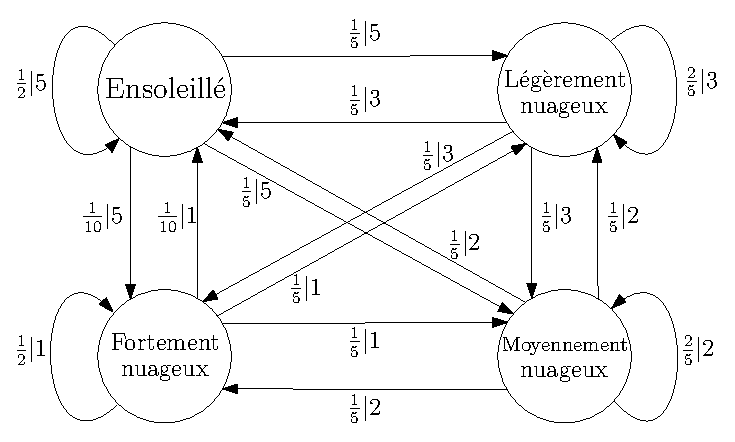
\includegraphics[scale=0.9]{figures/weather-solar-pannel.eps}
		\caption{Chaine de Markov pondérée de la production énergétique du système équipé de panneaux solaires en fonction du climat}
		\label{solar-pannel-1}
	\end{figure}
\end{example}

\begin{definition}[\textbf{Somme tronquée}]
	Soient $\mathcal{M} = (S, \Delta, w)$, une CMP, $T \subseteq S$, un sous-ensemble d'états cibles et $\pi = s_0s_1s_2 \dots \in Paths(\mathcal{M})$, un chemin dans $\mathcal{M}$. La \textit{somme tronquée} du chemin $\pi$ dans $\mathcal{M}$ pour $T$ est le coût total des transitions entre les états du chemin $\pi$ jusqu'à atteindre \textbf{pour la première fois} un des états cibles de $T$ (si le chemin n'atteint jamais un sommet de $T$, on dira que la somme tronquée est infinie).
	Plus précisément,
	soit $TS^T : Paths(\mathcal{M}) \rightarrow \mathbb{Z} \cup \{\infty\}$, la fonction qui calcule la somme tronquée de tout chemin vers l'ensemble cible $T$. La somme tronquée du chemin $\pi$ pour $T$ est définie par
	\[
		TS^T(\pi) =
		\begin{cases}
			\sum_{i = 0}^{n-1} w(s_i, s_{i+1}) & \quad \text{si } \forall i \in \{0, \dots, n - 1\}, s_i \notin T \text{ et } s_n \in T \\
			\infty & \quad \text{si } \pi \not \models \Diamond T,\; \ie \; \forall i \;\; s_i \notin T
		\end{cases}
	\]
\end{definition}

\begin{example}[\textit{Somme tronquée dans le système équipé de panneaux solaires}]
	Soit $\mathcal{M}_{sp}=(S, \Delta, w)$ la CMP de l'exemple \ref{solar-pannel-example}. On veut calculer l'énergie produite par les panneaux solaires cette semaine jusqu'à ce que le climat ait été fortement nuageux. On suppose que le temps était ensoleillé lundi, légèrement nuageux mardi et mercredi, ensoleillé jeudi, fortement nuageux vendredi et samedi ainsi que moyennement nuageux dimanche. Cette séquence forme un chemin $\pi = $\textit{ensoleillé, légèrement nuageux, légèrement nuageux, ensoleillé, fortement nuageux, fortement nuageux, moyennement nuageux, \dots} de $\mathcal{M}_{sp}$. Soit $T = \{\textit{fortement nuageux}\} \subseteq S$, l'ensemble cible. $TS^T(\pi) = 5 + 3 + 3 + 5 + 1 = 17$. Le système a donc produit $17\; kJ$ avant que le temps soit fortement nuageux.
\end{example}

%\begin{propriete}\label{prop-ts}
%	Soient $\mathcal{M} = (S, \Delta, w)$, une CMP, $s \in S$, un état de $S$ et $T \subseteq S$, un ensemble d'états cibles. On suppose que $0 < \pr_s(\Diamond T) < 1$. Alors, cela signifie que $\exists s' \in S \text{ et } \exists \pi = s_0 \dots s_n \in Paths_{fin}(s)$ tel que $s_0 = s,\; s_n = s',\; s_i \notin T \text{ pour tout } i \in \{0, \dots n \} \text{ et } \forall \pi' \in Paths(s'), \; \pi' \not \models \Diamond T$, \ie \textit{il existe un chemin fini (qui ne passe pas par un état de $T$) dans $\mathcal{M}$ commençant en l'état $s$ et qui mène à un état $s'$ tel que $s'$ ne peut jamais atteindre $T$ via n'importe quel chemin dans $\mathcal{M}$.}\\ Dès lors, $TS^T(\pi') = \infty$ et donc $TS^T(\pi \cdot \pi') = \infty$, \ie \textit{tous les chemins commençant en $s$ dont $\pi$ est préfixe n'atteignent jamais $T$ et mènent à une somme tronquée infinie.}
%\end{propriete}

\subsection{Problème de l'espérance du coût de l'accessibilité} \label{pb-esp-cout-acc}
Dans cette section, on s'intéresse à l'espérance (\cf définition \ref{espmath}) du coût des chemins qui atteignent un sous-ensemble d'états cibles d'une chaîne de Markov pondérée et plus précisément du coût total attendu pour qu'un état fixé atteigne un sous-ensemble d'états cibles.

\begin{definition}[\textbf{Espérance du coût de l'accessibilité}] \label{esp-access}
	Soient $\mathcal{M} = (S, \Delta, w)$, une CMP, $s \in S$, un état de $s$ et $T \subseteq S$, un ensemble d'états cibles. On définit l'espérance $\mathbb{E}_s(TS^T)$, correspondant au \textit{coût total attendu pour atteindre $T$ depuis $s$} comme suit :
	\begin{itemize}
	\renewcommand{\labelitemi}{\tiny$\bullet$}
	\item Si $\pr_s(\Diamond T) < 1$, alors $\mathbb{E}_s(TS^T) = \infty$.%(par la propriété \ref{prop-ts}).
		\\ En effet, soit $A = \{ \pi \in Paths(s) \; | \; \pi \models \Diamond T  \}$ et $B = \{ \pi \in Paths(s) \; | \; \pi \not \models \Diamond T  \}$. On sait que $\pr_s(\Diamond T) < 1 \; \implies \pr_s(B) > 0$, et donc, on a forcément que
		\[
			\mathbb{E}_s (TS^T) = \pr_s(A) \cdot \mathbb{E}_s(TS^T \; | \; A) + \pr_s(B) \cdot \underbrace{\mathbb{E}_s(TS^T \; | \; B)}_{ = \infty } = \infty
		\]
	\item Sinon, \ie si $\pr_s(\Diamond T) = 1$, alors :
	\[ \mathbb{E}_s(TS^T) = \sum_{c = 0}^\infty c \cdot \pr_s(\{\pi \in Paths(s) \; | \; TS^T(\pi) = c \})\]
	\end{itemize}
\end{definition}

\begin{proposition}
			Une définition équivalente de $\mathbb{E}_s(TS^T)$ dans le cas où $\pr_s(\Diamond T) = 1$ peut être donné par la moyenne du coût des chemins $\hat{\pi}$ pondérée par la probabilité de ces chemins $\hat{\pi}$ %alors que celui-ci se situe en l'état $s$
	, \ie
	\[\mathbb{E}_s(TS^T) = \sum_{\hat{\pi} \in Paths_{fin}^T(s)}\ \Delta(\hat{\pi}) \cdot TS^T(\hat{\pi})\]
\end{proposition}

\begin{proof}
	Soit $\pi = s_0 \dots s_n \dots \ \in Paths(s)$ tel que $\pi \models \Diamond T$. On suppose que $s_0 = s, \; \; s_i \notin T \; \text{ pour tout } i \in \{0, \dots, n-1\}$ et $s_n \in T$.  Soit $\hat{\pi} = s_0 \dots s_n \in Paths^T_{fin}(s)$. Alors, on a toujours que $TS^T(\pi) = TS^T(\hat{\pi})$.\\ \textit{(on peut ramener tout chemin infini $\pi$ qui atteint $T$ à un chemin fini $\hat{\pi}$ se terminant en la première occurrence d'un état de $T$ dans $\pi$ afin de calculer sa somme tronquée)}.
	\\Dès lors, soit $c \in \mathbb{N} \cup \{\infty\},$
	\begin{flalign}
		& c \cdot \pr_s(\{\pi \in Paths(s) \; | \; TS^T(\pi) = c \}) \notag\\
		& = c \cdot \pr_s(\{ \hat{\pi} \in Paths_{fin}^T(s) \; | \; TS^T(\hat{\pi}) = c\}) \notag\\
		& = c \cdot \sum_{\hat{\pi} \in Paths_{fin}^T(s) \; | \; TS^T(\hat{\pi}) = c} \Delta(\hat{\pi})
		\notag \\
		& = \sum_{\hat{\pi} \in Paths_{fin}^T(s) \; | \; TS^T(\hat{\pi}) = c} \Delta(\hat{\pi}) \cdot c \notag \\
		& = \sum_{\hat{\pi} \in Paths_{fin}^T(s) \; | \; TS^T(\hat{\pi}) = c} \Delta(\hat{\pi}) \cdot TS^T(\hat{\pi})
		\tag{car $c = TS^T(\hat{\pi})$}
	\end{flalign}
	Cela nous permet d'en déduire l'espérance de la façon suivante :
	\begin{flalign}
		\mathbb{E}_s(TS^T) &= \sum_{c=0}^\infty c \cdot \pr_s(\{\pi \in Paths(s) \; | \; TS^T(\pi) = c \}) \notag\\
		%\mathbb{E}_s(TS^T)
		&= \sum_{c=0}^\infty \quad \sum_{\hat{\pi} \in Paths_{fin}^T(s) \; | \; TS^T(\hat{\pi}) = c} \Delta(\hat{\pi}) \cdot TS^T(\hat{\pi}) \notag\\
		%\mathbb{E}_s(TS^T)
		&= \sum_{\hat{\pi} \in Paths_{fin}^T(s)}\ \Delta(\hat{\pi}) \cdot TS^T(\hat{\pi}) \notag
	\end{flalign}
\end{proof}

\subsubsection*{Système d'équations linéaires}
Soient $\mathcal{M} = (S, \Delta, w)$, une CMP \textbf{finie}, $s\in S$, un état de $S$ et $T \subseteq$ S, un ensemble d'états cibles. $\mathbb{E}_s(TS^T)$ peut se calculer via un système d'équations linéaires comme suit : \\
%Soient $x_s = \mathbb{E}_s(TS^T)$ %et $S_{=1} = \{s \in S \; | \; \mathbb{P}_s_s(\Diamond T) = 1 \}$
Soit $succ(s)$, l'ensemble des successeurs de $s$ dans $G^\mathcal{M}$,
\[ x_s =
	\begin{cases}
	\infty & \quad \text{si } \mathbb{P}_s(\Diamond T) < 1 \\
	0 & \quad \text{si } s \in T \\
	\sum_{s' \in succ(s)} \Delta(s, s') \cdot (w(s, s') + x_{s'}) & \quad \text{sinon}
	\end{cases}
\]

La probabilité d'un chemin fini $\hat{\pi} = s_0 s_1 \dots t \in Paths_{fin}^T(s)$, à savoir $\Delta(s_0 s_1 \dots t)$, peut se décomposer en $\Delta(s_0, s_1) \cdot \Delta(s_1 \dots t)$ et la somme tronquée de ce chemin, à savoir $TS^T(s_0 s_1 \dots t)$, en $w(s_0, s_1) + TS^T(s_1 \dots t)$. Intuitivement, cela mène au fait   que le coût moyen attendu pour atteindre l'ensemble d'états cibles depuis $s$ en passant par un de ses successeurs $s'$ peut se décomposer par le coût de la transition de $s$ vers le successeur $s'$ (à savoir $w(s, s')$) additionné à l'espérance du coût de l'accessibilité à l'ensemble d'états cibles depuis $s'$ (à savoir $\mathbb{E}_{s'}(TS^T)$). Afin de calculer l'espérance du coût de l'accessibilité à l'ensemble d'états cibles depuis $s$, le tout est ensuite pondéré par la distribution de probabilité de $s$ vers ses successeurs, et cela pour chacun de ses successeurs (\cf figure \ref{intuitionES}).

	\begin{figure}[H]
	\centering
	\captionsetup{justification=centering}
	\includegraphics[scale=0.75]{figures/intuitionES.eps}
	\caption{Intuition de l'espérance du coût de l'accessibilité à l'ensemble d'états cibles $T$ depuis l'état $s$, exprimé sous la forme $\mathbb{E}_s(TS^T) = \sum_{s' \in succ(s)} \Delta(s, s') \cdot \big( w(s, s') + \mathbb{E}_{s'}(TS^T) \big)$}
	\label{intuitionES}
\end{figure}

\subsubsection*{Généralisation matricielle}
Afin de résoudre ce système, on souhaite à présent définir un système matriciel équivalent possédant une unique solution.
\begin{theorem} \label{esp-theorem}
	Soit $S_{=1} = \{s \in S \; | \; \pr_s(\Diamond T) = 1 \}$. Le vecteur $(x_s)_{s \in S_{=1}}$ est l'unique solution du système d'équations
	\[
		x = Ax + b
	\]
	où
	\begin{itemize}
		\renewcommand{\labelitemi}{\tiny$\bullet$}
		\item $A \in \mathbb{Q}^{|S_{=1} \setminus T| \times |S_{=1} \setminus T|}$ tel que $\forall i, j \in \{1, \dots, |S_{=1} \setminus T | \}$, $A_{i, j} = \Delta(s_i, s_j)$. \\
		$(Ax)_i$ correspond donc à l'espérance moyenne attendue pour qu'un successeur ($\in S_{=1} \setminus T$) de $s_i \in S_{=1} \setminus T$  atteigne $T$.
		\item $b \in \mathbb{Q}^{|S_{=1} \setminus T|}$ tel que $\forall i \in \{1, \dots, |S_{=1} \setminus T |  \} ,\;b = \sum_{s' \in succ(s_i) %\cap S_{=1}
			} \Delta(s_i, s') \cdot w(s_i, s')$. \\
		$b_i$ correspond donc à l'espérance du coût engendré par l'action de quitter l'état $s_i \in S_{=1} \setminus T$ pour rejoindre un de ses successeurs $\in S_{=1}$.
	\end{itemize}
\end{theorem}

\textit{Intuition : } Soient $ s \in S_{=1} \setminus T$ et $i \in \{1, \dots, |S_{=1} \setminus T| \}$ tel que $s = s_i$,
\begin{flalign}
	x_s
		&= \sum_{s' \in succ(s)} \Delta(s, s') \cdot \big( w(s, s') + x_{s'} \big) \notag \\
		%&= \sum_{s' \in succ(s) \cap S_{=1}} \Delta(s, s') \cdot \big( w(s, s') + x_{s'} \big) \tag{car $s \in S_{=1} \implies s' \in succ(s) \in S_{=1}$} \\
		&= \sum_{s' \in succ(s) \cap S_{=1}} \Delta(s, s') \cdot x_{s'} + \sum_{s' \in succ(s) } \Delta(s, s') \cdot w(s, s') \notag \\
		&= \underbrace{\sum_{s' \in S_{=1} \setminus T} \Delta(s, s') \cdot x_{s'}}_{(Ax)_i} + \underbrace{\sum_{s' \in succ(s)} \Delta(s, s') \cdot w(s, s')}_{b_i} \tag{car $x_s = 0$ quand $s \in T$}
\end{flalign}

%\begin{proposition}
%	$x_s = \mathbb{E}_s(TS^T)$
%\end{proposition}
%\begin{proof}
%	On prouve que $x_s = {E}_s(TS^T)$ par récurrence. \\
%	\textbf{Cas de base :}
%	\begin{itemize}
%	\renewcommand{\labelitemi}{\tiny$\bullet$}
%		\item si $s \in T$, alors $x_s = 0$
%		\item si $\pr_s(\Diamond T) = 0$ (on peut le vérifier à partir de $G^\mathcal{M}$), alors $x_s = \infty$
%	\end{itemize}
%	\textbf{Cas général :} Soit $n = |succ(s)|$. On suppose que $\forall i \in \{0, \dots, n-1 \}$ tel que $s_i \in succ(s), \; x_{s_i} = E_{s_i}(TS^T)$.\\
%	Si $s \in T$ ou  $\pr_s(\Diamond T) = 0$, alors on est dans le cas de base. \\
%	Si $\exists i \in \{0, \dots, n-1 \}$ tel que $\pr(s_i \models \Diamond T) < 1$, alors $x_{s_i} = \infty$ et \[x_s = \sum_{i \in \{0, \dots, n-1\}} \Delta(s, s_i) \cdot (w(s, s_i) + x_{s_i}) = \infty\]
%	Sinon, alors $\forall i \in \{0, \dots, n-1 \},\; \pr(s_i \models \Diamond T) = 1$.\\
%	Il reste à prouver que $x_s = \sum_{s \cdot \hat{\pi}} \Delta(s \cdot \hat{\pi})  \cdot TS^T(s \cdot \hat{\pi})$\\
%	Soit $i \in \{0, \dots, n-1\}$. Supposons que $s_i \in T$. Alors,
%	\begin{flalign}
%		& \Delta(s, s_i) \cdot (w(s, s_i) + x_{s_i}) \notag \\
%		& = \Delta(s, s_i) \cdot w(s, s_i)  \tag{car $x_{s_i} = 0$} \\
%		& = \Delta(s, s_i) \cdot TS^T(s, s_i) \tag{a} \label{proof2-a}
%	\end{flalign}
%	Supposons à présent que $s_i \notin T$. Alors,
%	$x_{s_i} = \sum_{\hat{\pi}} \Delta(\hat{\pi}) \cdot TS^T(\hat{\pi})$ et
%	\begin{flalign}
%		& \; \Delta(s, s_i) \cdot (w(s, s_i) + x_{s_i}) \notag \\
%		= & \; \Delta(s, s_i) \cdot \Big(w(s, s_i) + \sum_{\hat{\pi} = s_i \dots t} \Delta(s_i \dots t) \cdot TS^T(s_i \dots t)\Big) \quad \text{$\forall t \in T$ tel que $\hat{\pi} \in Paths_{fin}^T$} \notag \\
%		= & \; %\underbrace{
%		\Delta(s, s_i) \cdot w(s, s_i)
%		%}_{\text{espérance du coût de $s$ vers ses successeurs}}
%		+ \sum_{\hat{\pi} = s_i \dots t} \Delta(s, s_i) \cdot \Delta(s_i \dots t) \cdot TS^T(s_i \dots t) \notag
%	\end{flalign}
%	\'Etant donné que $\pr(s_i \models \Diamond T) = 1$, que $s_i \notin T$ et que $\forall s, \sum_{s'} \Delta(s, s') = 1$, on a que
%	\begin{flalign}
%		\sum_{\hat{\pi} = s_i \dots t} \Delta(\hat{\pi}) &= 1 \notag \\
%		\iff \sum_{\hat{\pi} = s_i \dots t} \Delta(\hat{\pi}) \cdot w(s, s_i) &= w(s, s_i) \notag
%	\end{flalign}
%	Dès lors,
%	\begin{flalign}
%		& \;
%		\Delta(s, s_i) \cdot w(s, s_i)
%		+ \sum_{\hat{\pi} = s_i \dots t} \Delta(s, s_i) \cdot \Delta(s_i \dots t) \cdot TS^T(s_i \dots t)\notag \\
%		= & \;
%		\Delta(s, s_i) \cdot \Big(\sum_{\hat{\pi} = s_i \dots t} \Delta(s_i \dots t) \cdot w(s, s_i) \Big) + \Big(
%		 \sum_{\hat{\pi} = s_i \dots t} \Delta(s, s_i) \cdot \Delta(s_i \dots t) \cdot TS^T(s_i \dots t) \Big)\notag \\
%		 = & \;
%		 \sum_{\hat{\pi} = s_i \dots t} \Delta(s, s_i) \cdot \Delta(s_i \dots t) \cdot w(s, s_i) +
%		 \sum_{\hat{\pi} = s_i \dots t} \Delta(s, s_i) \cdot \Delta(s_i \dots t) \cdot TS^T(s_i \dots t) \notag \\
%		= & \sum_{\hat{\pi} = s_i \dots t} \Delta(ss_i \dots t) \cdot \Big(w(s, s_i) + TS^T(s_i \dots t) \Big) \notag \\
%		= & \sum_{\hat{\pi} = s_i \dots t} \Delta(ss_i \dots t) \cdot TS^T(ss_i \dots t) \tag{b} \label{proof2-b}
%	\end{flalign}
%	Par \ref{proof2-a} et \ref{proof2-b}, on a :
%	\begin{flalign}
%		& \sum_{i \in \{0, \dots, n-1 \}} \Delta(s, s_i) (w(s, s_i) + x_{s_i}) \notag \\
%		= & \quad \sum_{s \cdot \hat{\pi}} \Delta(s \cdot \hat{\pi}) \cdot TS^T(s \cdot \hat{\pi}) \notag
%	\end{flalign}
%\end{proof}

\begin{example}[\textit{Espérance de la production énergétique du système de panneaux solaires}]
	Cet exemple se base sur la CMP $\mathcal{M}_{sp} = (S, \Delta, w)$ de l'exemple \ref{solar-pannel-example}. On souhaite connaitre l'espérance de la production énergétique des panneaux solaires lorsque le climat est ensoleillé jusqu'à ce que le climat devienne fortement nuageux et cela dans le but de connaitre la production énergétique attendue que peut avoir un tel système au moment où sa production est maximale jusqu'à son niveau de production minimale due au climat.\\
	Soit $s \in S$ et $T = {\text{fortement nuageux}}$. On a $x_s = \mathbb{E}_s(TS^T)$. Le graphe $G^{\mathcal{M}_{sp}}$ est fortement connexe, on a donc $x_s \neq \infty$. Le système d'équations linéaires correspondant s'écrit :

\begin{flalign}
	&\begin{cases}
		x_{e} = \frac{1}{2} (5 + x_e) +
			\frac{1}{5} (5 + x_{ln}) +
			\frac{1}{5} (5 + x_{mn}) +
			\frac{1}{10} (5 + x_{fn}) \\
		x_{ln} = \frac{2}{5} (3 + x_{ln}) +
			\frac{1}{5} (3 + x_e) +
			\frac{1}{5} (3 + x_{mn}) +
			\frac{1}{5} (3 + x_{fn}) \\
		x_{ln} = \frac{2}{5} (2 + x_{mn}) +
			\frac{1}{5} (2 + x_e) +
			\frac{1}{5} (2 + x_{ln}) +
			\frac{1}{5} (2 + x_{fn}) \\
		x_{fn} = 0
	\end{cases}
	\notag\\
	\iff &\begin{cases}
		\frac{1}{2} x_e - \frac{1}{5} x_{ln} - \frac{1}{5} x_{mn} - \frac{1}{10}x_{fn} =5 \\
		\frac{-1}{5} x_e + \frac{3}{5} x_{ln} + \frac{1}{5} x_{mn} - \frac{1}{5} x_{fn} =3 \\
		\frac{-1}{5} x_e - \frac{1}{5} x_{ln} + \frac{3}{5} x_{mn} - \frac{1}{5} x_{fn} = 2 \\
		x_{fn} = 0
	\end{cases} \notag
\end{flalign}
{\footnotesize \textit{Note} : Par souci de visibilité, \textit{e = ensoleillé, ln = légèrement nuageux, mn = moyennement nuageux et fn = fortement nuageux}}. \\
Afin de résoudre ce système, il est utile de le passer sous forme matricielle par le théorème \ref{esp-theorem}  :
\[
\begin{pmatrix}
\frac{1}{2} & \frac{-1}{5} & \frac{-1}{5}\\[0.3em]
\frac{-1}{5} & \frac{3}{5} & \frac{-1}{5}\\[0.3em]
\frac{-1}{5} & \frac{-1}{5} & \frac{3}{5}

\end{pmatrix}
\;
\begin{pmatrix}
x_{e} \\[0.3em] x _{ln} \\[0.3em] x_{mn}
\end{pmatrix}
= \;
\begin{pmatrix}
\;5 \; \\[0.3em] \; 3 \; \\[0.3em] \; 2 \;
\end{pmatrix}
\]
On résout encore une fois ce système d'équations linéaires par le pivot de Gauss. La solution du système est :
\[ x_e = 25, \; x_{ln} = 19.375, \; x_{mn} = 18.125, \; x_{fn} = 0  \]
De ce fait, $\mathbb{E}_{\textit{ensoleillé}} (TS^{\{\textit{fortement nuageux}\}}) = 25\; kJ$.
\end{example}

\subsection{Problème d'accessibilité limitée par un coût}
Dans le problème précédent, on était intéressé par le coût moyen attendu pour qu'un état du système atteigne un sous-ensemble d'états cibles. Avec le \textit{problème d'accessibilité limitée par un coût}, on s'intéresse plutôt à la probabilité que cet état atteigne le sous-ensemble d'états cibles avec un coût inférieur à un seuil fixé au préalable.

\begin{definition}[\textbf{Accessibilité limitée par un coût}]\label{acc-lim}
	Soient $\mathcal{M} = (S, \Delta, w)$, une CMP, $s \in S$, un état, $T \subseteq S$, un sous-ensemble d'états cibles et $b \in \mathbb{Z}$, un seuil. La \textit{probabilité d'atteindre $T$ depuis $s$ limitée par un coût} de seuil $b$ est définie comme suit :
	\[\pr_s(TS^T \leq b) = \pr_s(\{\pi \in Paths(s) \; | \; TS^T(\pi) \leq b \}) \]
\end{definition}

\begin{notation}
Soit $\mathcal{M} = (S, \Delta, w)$, une CMP. On désigne par $\pr^\mathcal{M}_s$ la mesure de probabilité $\pr_s$ telle que $s \in S$ est un état de la CMP $\mathcal{M}$.
\end{notation}

\subsubsection*{Réduction au problème d'accessibilité}
Soient $\mathcal{M} = (S, \Delta, w)$, une CMP, $s \in S$, un état du système, $T \subseteq S$, un ensemble d'états cibles et $b \in \mathbb{Z}$, un seuil. Afin de résoudre $\pr_s(TS^T \leq b)$, on réduit le problème à un simple problème d'accessibilité sur la CM $\mathcal{M}' = (S', \Delta')$ pour le sous-ensemble d'états cibles $T' \subseteq S'$, que l'on construit comme suit :
\begin{itemize}
	\renewcommand{\labelitemi}{\tiny$\bullet$}
	\item $S'$ est un ensemble de tuples $(s, v)$ tel que $s \in S $ et $v \in \mathbb{N} \cup \{ \bot \}$. On considère que $\bot > b$, avec $\bot + v = \bot \; \; \forall v \in \mathbb{N}$. Intuitivement, on enregistre dans $v$ le coût total du chemin en parcourant $\mathcal{M}$. Les états cibles sont donc les états de $T' = \{ (s, v) \in S' \; | \; s \in T \wedge v \leq b \}$.
	\item $\Delta': S' \times S' \rightarrow [0,1]$ est la fonction de probabilité de transition définie comme suit :\\
	$\forall (s, v), (s', v') \in S',$
	\[
		\Delta'((s, v), (s', v')) =
		\begin{cases}
		\Delta(s, s') & \text{si $v' = v + w(s, s')$ et $v' \leq b$  ou} \\
		 & \text{si $v' = \bot$ et $v + w(s, s') > b$} \\
		 0 & \text{ sinon}
		\end{cases}
	\]

%\begin{remark}
%	Nous ne sommes intéressés que par les chemins dont le coût total (\ie la somme tronquée) est inférieur à $b$. De ce fait, tout état $(s, v) \in S'$ tel que $v = \bot$ n'est utile au système que pour identifier les chemins qui ont dépassé le seuil $b$. Soient $\mathcal{M^*}$, une CM qu'on a construit à partir de $\mathcal{M}$ telle que $\mathcal{M^*} = (S', \Delta^*)$ et $S^* \subseteq S'$, l'ensemble des états $(s, v) \in S'$ tel que $v = \bot$. Par le fait que $T' \cap S^* = \emptyset$ ainsi que par le fait que $\forall (s, v) \in S^*$, tout chemin $\pi$ de $\mathcal{M^*}$ tel que $\pi \in Paths((s, v))$ vérifie $\pi \not \models \Diamond T'$, on peut remplacer tout état de $S^*$ dans $\mathcal{M^*}$ par un seul état absorbant $(s^*, \bot)$ dans $\mathcal{M'}$ . \\
%\end{remark}
%
%\item $\Delta': S' \times S' \rightarrow [0,1]$ est la fonction de probabilité de transition de $\mathcal{M'}$ et est définie comme suit : \\
%	$\forall (s, v), (s', v') \in S',$
%\[
%\Delta'((s, v), (s', v')) =
%\begin{cases}
%\Delta(s, s') & \text{\quad \, si $v' = v + w(s, s')$ et $v' \leq b$}  \\
%	& %\quad \quad \;\,
%	\quad \;\, \text{et $s \notin T$} \\
%\sum_{(s_\bot, v_\bot) \in S' | v_\bot = \bot} \Delta^*((s, v), (s_\bot, v_\bot)) & \quad \, \text{ si $s' = s^*$ et $v' = \bot$} \\
%1 & \quad \, \text{ si $s = s' \in T$ et $v = v'$} \\
%& \text{ou si $s = s' = s^*$ et $v = v' = \bot$} \\
%0 & \quad \, \text{ sinon}
%\end{cases}
%\]
\end{itemize}
 Dès lors, on a \[\pr^\mathcal{M}_s(\{\pi \in Paths(s) \; | \; TS^T(\pi) \leq b \}) = \pr^\mathcal{M'}_{(s, 0)}(\Diamond T')\]
\ie résoudre le problème d'accessibilité de $s$ à $T$ dans $\mathcal{M}$ limitée par le coût de seuil $b$ revient à résoudre le problème d'accessibilité de $(s, 0)$ à $T'$ dans $\mathcal{M'}$. \\

\begin{example}[\textit{Accessibilité limitée par un coût dans le système équipé de panneaux solaires}]
	On reprend la CMP $\mathcal{M}_{sp} = (S, \Delta, w)$ de l'exemple \ref{solar-pannel-example}.
	%On suppose que l'installation de panneaux solaire est rentable lorsque celle-ci produit au moins $8\; kJ$ lorsque le climat est ensoleillé jusque quand le climat est fortement nuageux.
	On souhaite connaitre la probabilité que le système équipé de panneaux solaires produise \textbf{au moins $8 \; kJ$} avant que le climat soit fortement nuageux, en supposant que l'installation commence à produire l'énergie un jour ensoleillé.\\
	Pour ce faire, on va d'abord déterminer la probabilité que le système produise moins de $7\; kJ$, \ie $\pr_{\textit{ensoleillé}}(TS^{\{ \textit{fortement nuageux} \}} \leq 7)$. On réduit le problème à un problème d'accessibilité en construisant la CM $\mathcal{M'}_{sp} = (S', \Delta')$ comme décrit ci-dessus (\cf figure \ref{figure-cbr-03}).

\begin{figure}[H]
	\centering
	\captionsetup{justification=centering}
	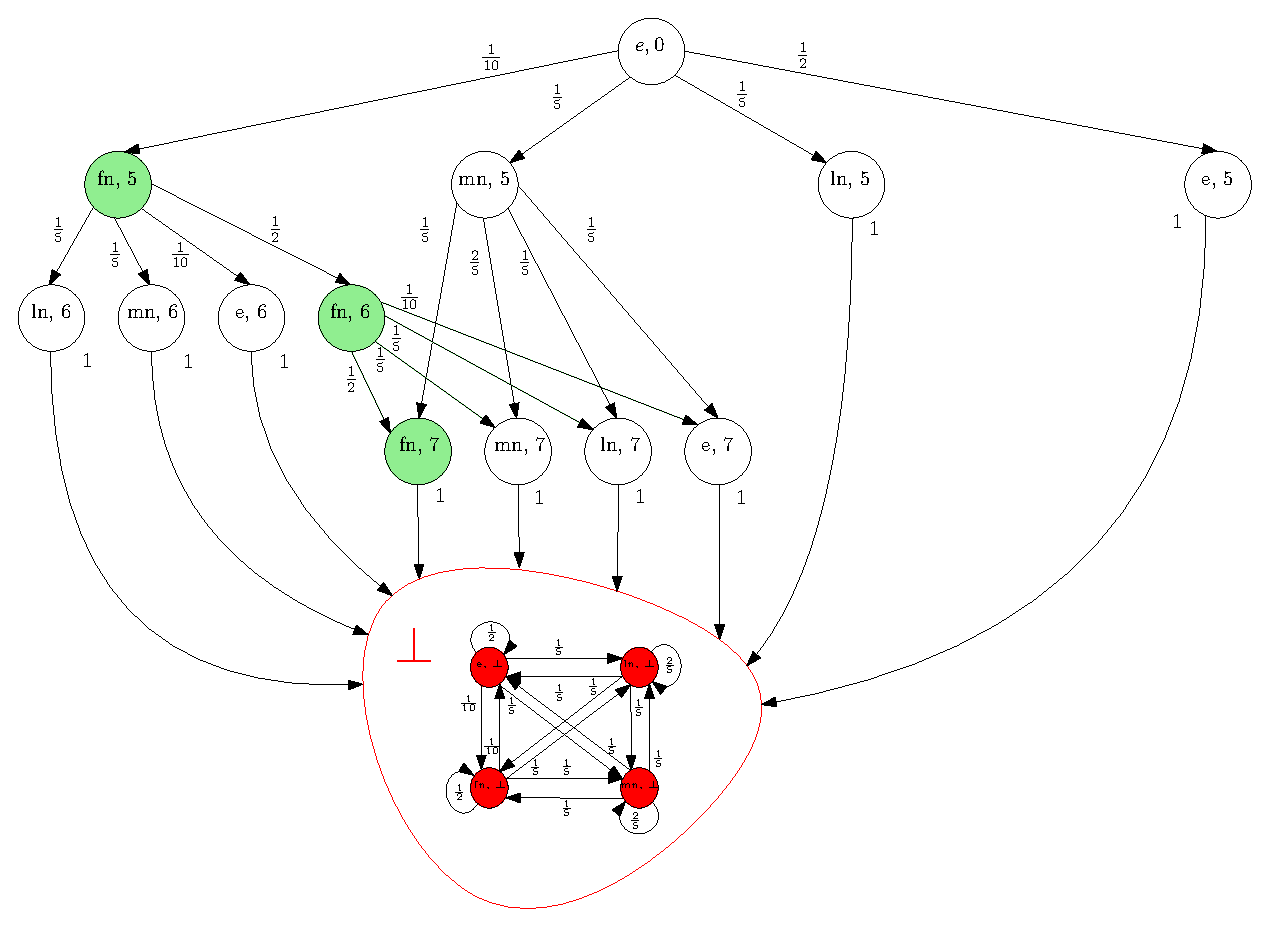
\includegraphics[scale=0.7]{figures/limited-reachability-example2.eps}
	\caption{CM $\mathcal{M'}_{sp}$ construite à partir de $\mathcal{M}_{sp}$ afin de résoudre $\pr_{\textit{ensoleillé}}(TS^{\{ \textit{fortement nuageux} \}} \leq 7)$}
	\label{figure-cbr-03}
\end{figure}
Par le théorème \ref{reachability-theorem}, on peut résoudre ce problème d'accessibilité de la façon suivante :
\begin{itemize}
	\renewcommand{\labelitemi}{\tiny$\bullet$}
	\item $S_{=1} = T' = \{(fn, 5), (fn, 6), (fn, 7)\}$. Donc, $\forall s \in S_{=1}, \; \pr_s^\mathcal{M'}(\Diamond T') = 1$.
	\item $S_{=0}$ est l'ensemble des états non-connexes à $T'$. On a donc que $S_{=0} =$ $\{(ln, 5), $(e, 5), (ln, 6), $(mn, 6), (mn, 7),(ln, 7),$ $(e, 7), (e, \bot), (ln, \bot), $$(mn, \bot), (fn, \bot) \}$ et que $\forall s \in S_{=0}, \; \pr_s^\mathcal{M'} (\Diamond T') = 0$
	\item Il reste à déterminer $\pr_s^\mathcal{M'} (\Diamond T')\; \forall s\in S_{?}$ tel que $S_? = S \setminus (S_{=1} \cup S_{=0})$. Pour ce faire, on résout le système matriciel suivant :
	\begin{flalign*}
		\begin{pmatrix}
			0 & \frac{1}{5}\\[0.3em]
			0 & 0
		\end{pmatrix}
			\;
		\begin{pmatrix}
			x_{(e, 0)}\; \\[0.3em]
			x_{(mn, 5)}\;
		\end{pmatrix}
		\; + \;
		\begin{pmatrix}
			\frac{1}{10}\\[0.3em]
			\frac{1}{5}
		\end{pmatrix}
		\; &= \;
		\begin{pmatrix}
			x_{(e, 0)}\; \\[0.3em]
			x_{(mn, 5)}\;
		\end{pmatrix}\\ \iff
		\begin{pmatrix}
			1 & - \frac{1}{5}\\[0.3em]
			0 & 1
		\end{pmatrix}
		\;
		\begin{pmatrix}
			x_{(e, 0)}\; \\[0.3em]
			x_{(mn, 5)}\;
		\end{pmatrix}
		\; &= \;
		\begin{pmatrix}
			\frac{1}{10}\\[0.3em]
			\frac{1}{5}
		\end{pmatrix} \\
		 \iff
		\begin{pmatrix}
		x_{(e, 0)}\; \\[0.3em]
		x_{(mn, 5)}\;
		\end{pmatrix}
		\; &= \;
		\begin{pmatrix}
		0.14\\[0.3em]
		\frac{1}{5}
		\end{pmatrix}
	\end{flalign*}
\end{itemize}
%Dès lors, $T' = \{ (fn, 5), (fn, 6), (fn, 7) \}$. On a donc que $P_{(fn, 5)}^\mathcal{M'}(\Diamond T)=P_{(fn, 6)}^\mathcal{M'}(\Diamond T) = P_{(fn, 7)}^\mathcal{M'}(\Diamond T) = 1$. De plus, les états $(ln, 5)$, $(e, 5)$, $(ln, 6)$, $(mn, 6)$, $(mn, 7)$, $(ln, 7)$, $(e, 7)$, $(e, \bot)$, $(ln, \bot)$, $(mn, \bot)$ ainsi que $(fn, \bot)$ ne sont pas connexes à $T$. De ce fait, la probabilité que ces états atteignent l'ensemble d'états cibles $T$ est nulle. Par le théorème \ref{reachability-theorem}, on peut résoudre le problème d'accessibilité via le système matriciel suivant :
%\begin{flalign}
%	&x_{(LN, 5)} = x_{(E, 5)} = x_{(MN, 7)} = x_{(E, 7)} = x_{(s^*, \bot)} = 0 \notag \\
%	&\begin{cases}
%		x_{(E, 0)} = \frac{1}{5} x_{(MN, 5)} + \frac{1}{5} x_{(LN, 5)} + \frac{1}{2} x_{(E, 5)} + \frac{1}{10} \\
%		x_{(MN, 5)} = \frac{2}{5} x_{(MN, 7)} + \frac{1}{5} x_{(LN, 7)} + \frac{1}{5} x_{(E, 7)} + \frac{1}{5}
%	\end{cases}\notag \\
%	\iff &
%	\begin{cases}
%		x_{(E, 0)} = \frac{1}{5} x_{(MN, 5)} + \frac{1}{10} \\
%		x_{(MN, 5)} = \frac{1}{5}
%	\end{cases}\notag \\
%	\implies& x_{(E, 0)} = \frac{7}{50} = 0.14 \notag
%\end{flalign}
On a $\pr^{\mathcal{M'}}_{(e, 0)} (\Diamond T') = \pr^\mathcal{M}_{\textit{ensoleillé}}(TS^{\{ \textit{fortement nuageux} \}} \leq 7) = 0.14$. On revient au problème initial. On veut connaitre $\pr_{\textit{ensoleillé}}(TS^{\{ \textit{fortement nuageux} \}} > 7)$. Comme $\pr_{\textit{ensoleillé}}$ est une mesure de probabilité, on a par la propriété \ref{negproba} \[1 - \pr_{\textit{ensoleillé}}(TS^{\{ \textit{fortement nuageux} \}} \leq 7) = \pr_{\textit{ensoleillé}}(TS^{\{ \textit{fortement nuageux} \}} > 7)\]
On a $\pr_{\textit{ensoleillé}}(TS^{\textit{fortement nuageux}} > 7) =
\pr_{\textit{ensoleillé}}(TS^{\textit{fortement nuageux}} \geq 8)$ car la production est entière,
et donc, on a $\pr_{\textit{ensoleillé}}(TS^{\{ \textit{fortement nuageux} \}} \geq 8) = 0.86$.
\end{example}

%\begin{example}[\textit{Réduction au problème d'accessibilité}]
%	Pour cet exemple, reprenons la CM de l'exemple \ref{reachex} en ajoutant des poids sur les transitions. On obtient la CMP $\mathcal{M}_{cbr}$ (\cf figure \ref{figure-cbr-01}).
%
%	\begin{figure}[H]
%		\centering
%		\includegraphics[scale=0.7]{figures/cost-bounded-reachability01.eps}
%		\caption{Chaine de Markov pondérée $\mathcal{M}_{cbr}$}
%		\label{figure-cbr-01}
%	\end{figure}
%
%	On souhaite connaitre la probabilité que le fait de ne pas emprunter la transition $(s_0, s_6)$ soit avantageux au niveau du coût total pour atteindre les états $s_5$ ou $s_6$ depuis $s_0$, ou encore la probabilité d'atteindre les états $s_5$ ou $s_6$ depuis l'état $s_0$ avec un coût strictement inférieur à $5$ \ie $\pr_{s_0}(\{ \pi \in Paths(s_0) \; | \; TS^T(\pi) \leq 4 \})$. Pour cela, on réduit le problème à un problème d'accessibilité sur la CMP $\mathcal{M}'_{cbr}$ (\cf figure \ref{figure-cbr-02}). Dès lors, l'ensemble d'états cibles est $T' = \{ (s_5, 4), (s_5, 3), (s_6, 4) \}$.
%
%	\begin{figure}[H]
%		\centering
%		\includegraphics[scale=0.5]{figures/cost-bounded-reachability02.eps}
%		\caption{CMP $\mathcal{M'}_{cbr}$ construite à partir de $\mathcal{M}_{cbr}$ dans le but de résoudre le problème $\pr_{s_0}(\{ \pi \in Paths(s_0) \; | \; TS^T(\pi) \leq 4 \})$ }
%		\label{figure-cbr-02}
%	\end{figure}
%\end{example}

\chapter{Processus Décisionnels de Markov}

Les chaînes de Markov ne permettent pas de modéliser des situations probabilistes impliquant des prises de décisions. Avec les \textit{processus décisionnels de Markov}, de telles situations peuvent être modélisées. \`A chaque étape, le système se trouve en un état de prise de décision et une action doit être choisie. Une fois que l'action est choisie, le comportement du système devient probabiliste, comme lorsqu'on passe d'un état à un autre dans une chaîne de Markov. Dans un tel système, la transition d'un état à un autre dépend donc d'abord de l'action choisie, et ensuite de la distribution de probabilité définie par l'état actuel du système ainsi que par l'action choisie. \\

Ce chapitre est essentiellement inspiré du chapitre \textit{Probabilistic Systems} du livre \textit{Principles of model checking} \cite{DBLP:books/daglib/0020348} ainsi que de l'article \textit{Variation on
the Stochastic Path Problem} \cite{DBLP:journals/corr/RandourRS14a}.

\section{Définitions et propriétés}

\begin{definition}[\textbf{Processus décisionnel de Markov}]
	Un \textit{processus décisionnel de Markov}, noté \textbf{PDM} est un tuple $\mathcal{M}  = (S, A, \Delta)$ où
	\begin{itemize}
		\renewcommand{\labelitemi}{\tiny $\bullet$}
		\item $S$ est un ensemble dénombrable d'états.
		\item $A$ est un ensemble dénombrable d'actions. On dénote par $A(s) \in \mathcal{P}(A)$  l'ensemble des actions possibles lorsque le système se trouve dans l'état $s$. Pour tout état $s \in S$, on a toujours que $A(s) \neq \varnothing$.
		\item $\Delta: S \times A \times S \rightarrow [0, 1] \cap \mathbb{Q}$ est la fonction de transition telle que
		\begin{flalign*}
			&\forall s \in S, \; \forall \alpha \in A(s), \; \sum_{s' \in S} \Delta(s, \alpha, s') = 1 \\
			\text{et } &\forall s, s' \in S, \; \forall \alpha \in A \setminus A(s), \; \Delta(s, \alpha, s') = 0
		\end{flalign*}

			$\Delta$ spécifie, pour tout état $s \in S$, la probabilité que le système passe de l'état $s$ à $s'$ lorsque l'action $\alpha \in A(s)$ est choisie.
	\end{itemize}
\end{definition}

\begin{propriete}
	Soient $\mathcal{M} = (S, A, \Delta)$, un PDM, $s \in S$ un état de $\mathcal{M}$ et $\alpha \in A(s)$, une action possible lorsque le PDM $\mathcal{M}$ est en $s$. Les contraintes imposées sur $\Delta$ assurent que $\Delta_{s, \alpha}$ est une distribution de probabilité sur $S$ (\cf définition \ref{distriprobadef}) où
	\[
		\Delta_{s, \alpha} : S \rightarrow [0, 1] \cap \mathbb{Q}, \; s' \mapsto \Delta(s, \alpha, s')
	\]
\end{propriete}

Soient $\mathcal{M} = (S, A, \Delta)$, un PDM et $s \in S$ un état de $\mathcal{M}$. Au moment où le système entre dans l'état $s$, un choix doit être effectué afin de passer à l'étape suivante. En effet, supposons que $A(s) = \{\alpha, \beta\}$. Une action possible de $\{\alpha, \beta \}$ doit être choisie, ce qui implique qu'on ne
peut pas savoir quels seront les successeurs possibles de $s$ tant qu'une action
n'aura pas été choisie. Cela rend ce choix purement \textbf{non-déterministe}.
\begin{figure}[H]
	\centering
	\includegraphics[scale=0.7]{figures/PDM-intuition.eps}
	\caption{Extrait du Processus décisionnel de Markov $\mathcal{M}$}
\end{figure}
On suppose alors que l'action $\alpha$ est sélectionnée. Lorsque $\alpha$ est choisie, le \textit{successeur-}$\alpha$ de $s$ est choisi aléatoirement selon la distribution de probabilité $\Delta_{s, \alpha}$. Donc, $s' \in S$ est successeur de $s$ avec une probabilité de $\Delta(s, \alpha, s')$.


\begin{notation}
	Soit $\mathcal{M} = (S, A, \Delta)$, un PDM.
		%\item $\Delta(s, \alpha, T)$ dénote la probabilité que le système, se trouvant en
		%	l'état $s$, évolue en l'un
		%	des états du sous-ensemble d'états $T \subseteq S$ en choisissant l'action
		%	$\alpha \in A(s)$, i.e.,
		%	\[ \Delta(s, \alpha, T) = \sum_{t \in T} \Delta(s, \alpha, t) \]
		$Succ(s, \alpha)$ dénote l'ensemble des \textit{successeurs}-$\alpha$ de l'état $s
			\in S$, i.e.,
			\[ Succ(s, \alpha) = \{ s' \in S \; | \; \Delta(s, \alpha, s') > 0 \} \]
		%\item $Pred(s')$ dénote l'ensemble des paires $(s, \alpha)$ qui précèdent $s'$
		%dans $\mathcal{M}$ telles que $s \in S$
		%est un état de $\mathcal{M}$ et $\alpha \in A(s)$ est une action possible lorsque
		%le système se trouve en l'état $s$. Dès lors, on définit les prédecesseurs de $s'$ comme suit :
		%\[ Pred(s') = \{ (s, \alpha) \in S \times A \; | \; \Delta(s, \alpha, s') > 0
		%\} \]
\end{notation}

\begin{remark}
	Si $s'$ est l'unique successeur-$\alpha$ de $s$, alors, on a que $\Delta(s, \alpha, s') = 1$
	et que $\Delta(s, \alpha, s^*) = 0$ pour tout $s^* \neq s'$.
	Dans ce cas, il n'est pas nécessaire de représenter l'actions $\alpha$
	dans la représentation du PDM.
\end{remark}

\begin{example}[\textit{Agent dans un labyrinthe stochastique}] \label{maze-agent}
Afin d'illustrer ces concepts, on se base sur un exemple personnel. Un agent ère dans un labyrinthe (cf. figure \ref{maze-figure}). Son but est d'atteindre les cases cibles
$t_1$ et $t_2$. Lorsqu'il se déplace
dans le labyrinthe, l'agent doit décider, à chaque case, la
direction dans laquelle se diriger à la prochaine étape. Cependant, l'agent
ne peut pas prendre la décision de revenir sur ses pas, i.e., de se
diriger dans la case dans laquelle il se trouvait à l'étape précédente,
à moins d'y être contraint.
On suppose que l'environnement
du labyrinthe est stochastique. En effet, certaines cases du
labyrinthe regorgent de pièges, ce qui peut contraindre l'agent à changer de
direction. Dans le cas des cases dans lesquelles il y a la présence de pièges, l'agent a le droit de décider de faire demi-tour.
On considère ici que les pièges sont simples et consistent à forcer l'agent à
prendre une direction différente de celle issue de la prise de décision.
La liste des pièges est la suivante :
\begin{itemize}
	\renewcommand{\labelitemi}{\tiny$\bullet$}
	\item case $(1, 1)$ : le piège a $20 \%$ de chance de s'activer.
	\item case $(1, 3)$ : lorsque l'agent essaie de rejoindre la case $(2, 3)$,
		i.e., lorsque l'agent décide de se diriger vers le sud, le piège a
		une chance sur trois de s'activer. Si l'agent choisit une autre direction, le piège a $10 \%$ de chance
		d'activation, mais ne contraint pas l'agent à se diriger dans la direction
		opposée à celle choisie.
	\item case $(4, 3)$ : lorsque l'agent essaie de rejoindre la case $t_1$, i.e., lorsque l'agent décide de se diriger vers le nord, le piège a une chance sur cinq de s'activer. Si l'agent choisit une autre
		direction, alors le piège a $10 \%$ de chance d'activation. Cependant, le piège ne
		contraint pas l'agent à revenir sur ses pas.
\end{itemize}
	\begin{figure}[H]
		\centering
		\captionsetup{justification=centering}
		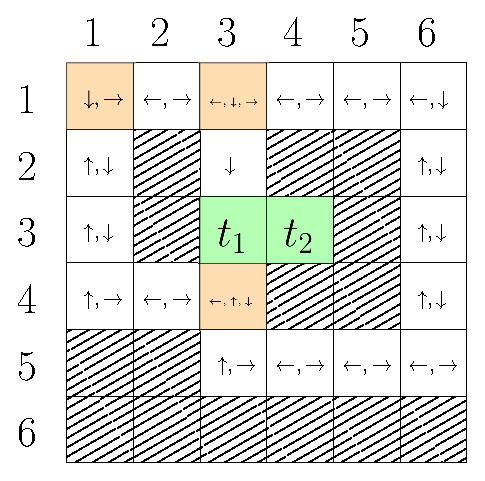
\includegraphics[scale=0.8]{figures/maze}
		\caption{Labyrinthe dans lequel un agent tente de rejoindre les cases $t_1$ et $t_2$.
			Les directions indiquées dans les cases sont les choix possibles de
			l'agent lorsqu'il se situe dans ces cases. Les cases en orange
			représentent les cases dans lesquelles des pièges sont présents, pouvant
			forcer l'agent à prendre une direction différente.}
		\label{maze-figure}
	\end{figure}
	On peut modéliser cette situation sous la forme d'un PDM
	$\mathcal{M}_{\text{maze}} = (S, A, \Delta)$ (cf. figure \ref{PDM-maze-figure}). Comme l'agent ne peut pas
	prendre la décision de revenir sur ses pas, il n'est pas intéressant de considérer
	toutes les cases comme états du système. On considère donc uniquement les
	cases qui requièrent une prise de décision ainsi que les états cibles.
	On a donc
	$S = \{ (1,1), (1,3), (4,3), t_1, t_2 \}$. On a ensuite $4$ prises de
	décisions possibles au total. Il s'agit des actions de $A = \{ \leftarrow,
	\rightarrow, \uparrow, \downarrow \}$.
	\begin{figure}[H]
		\centering
		\captionsetup{justification=centering}
		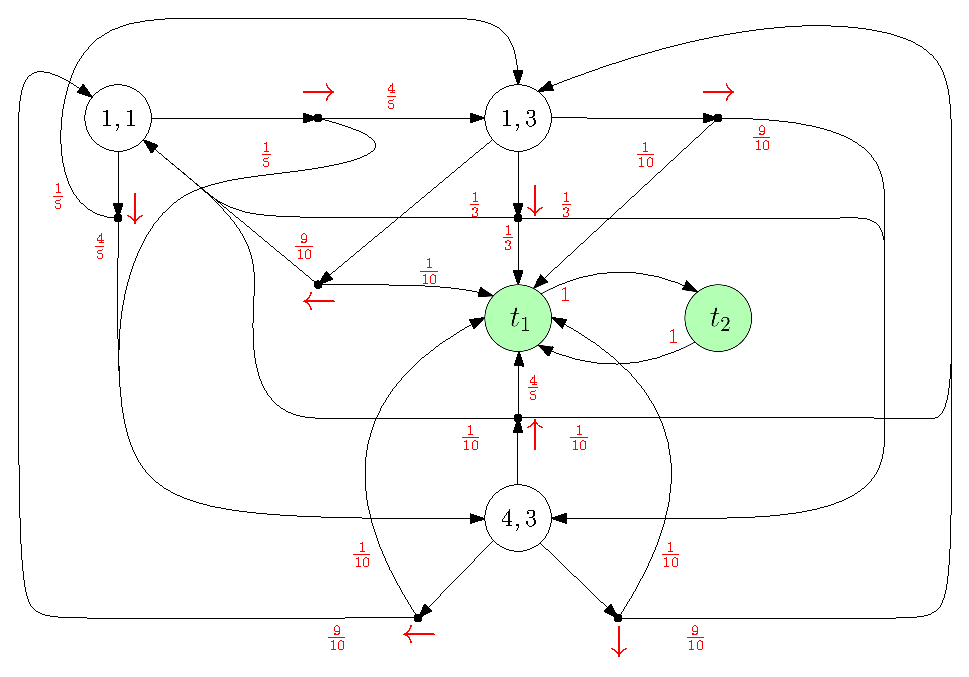
\includegraphics[scale=0.75]{figures/mazePDM}
		\caption{PDM $\mathcal{M}_{\text{maze}}$.}
		\label{PDM-maze-figure}
	\end{figure}

	En pratique, et à plus grande échelle, on peut considérer un véhicule autonome comme étant un agent,
	qui a connaissance de son environnement, correspondant au labyrinthe, via les cartes fournies par un GPS.
	Il est évident que l'environnement dans lequel ce véhicule se déplacerait
	est stochastique (e.g. voies bloquées, bouchons non renseignés par les
	données provenant du GPS et autres évènements dont l'agent ne peut pas
	avoir connaissance). Ces évènements sont considérés comme étant
	les pièges présents dans certaines cases du labyrinthe.

\end{example}

\begin{propriete} \label{PDM=CM}
	Toute CM est un PDM tel que pour tout état $s$, un seul choix d'action est
	possible à chaque étape, i.e., $|A(s)| = 1$. La réciproque est également vraie, tout
	PDM possédant cette propriété (i.e., pour tout état $s$, $|A(s)| = 1$) est une
	CM. Dans ce cas, représenter les actions de $A(s)$ dans la représentation du PDM n'est plus pertinent et peut être omis.
\end{propriete}

%\begin{example}[\textit{PDM du dé de Knuth}]
%Reprenons la CM de l'exemple \ref{knuthdie} (dé de Knuth). Selon la propriété \ref{PDM=CM},
%il existe un PDM équivalent (cf. figure \ref{PDM=CM-example}).
%	\begin{figure}[H]
%		\captionsetup{justification=centering}
%		\begin{minipage}{0.45\textwidth}
%				\centering
%				\includegraphics[scale=0.4]{figures/dieByaCoin.eps}
%		\end{minipage}
%		\hspace{0.05\textwidth}
%		\begin{minipage}{0.45\textwidth}
%				\centering
%				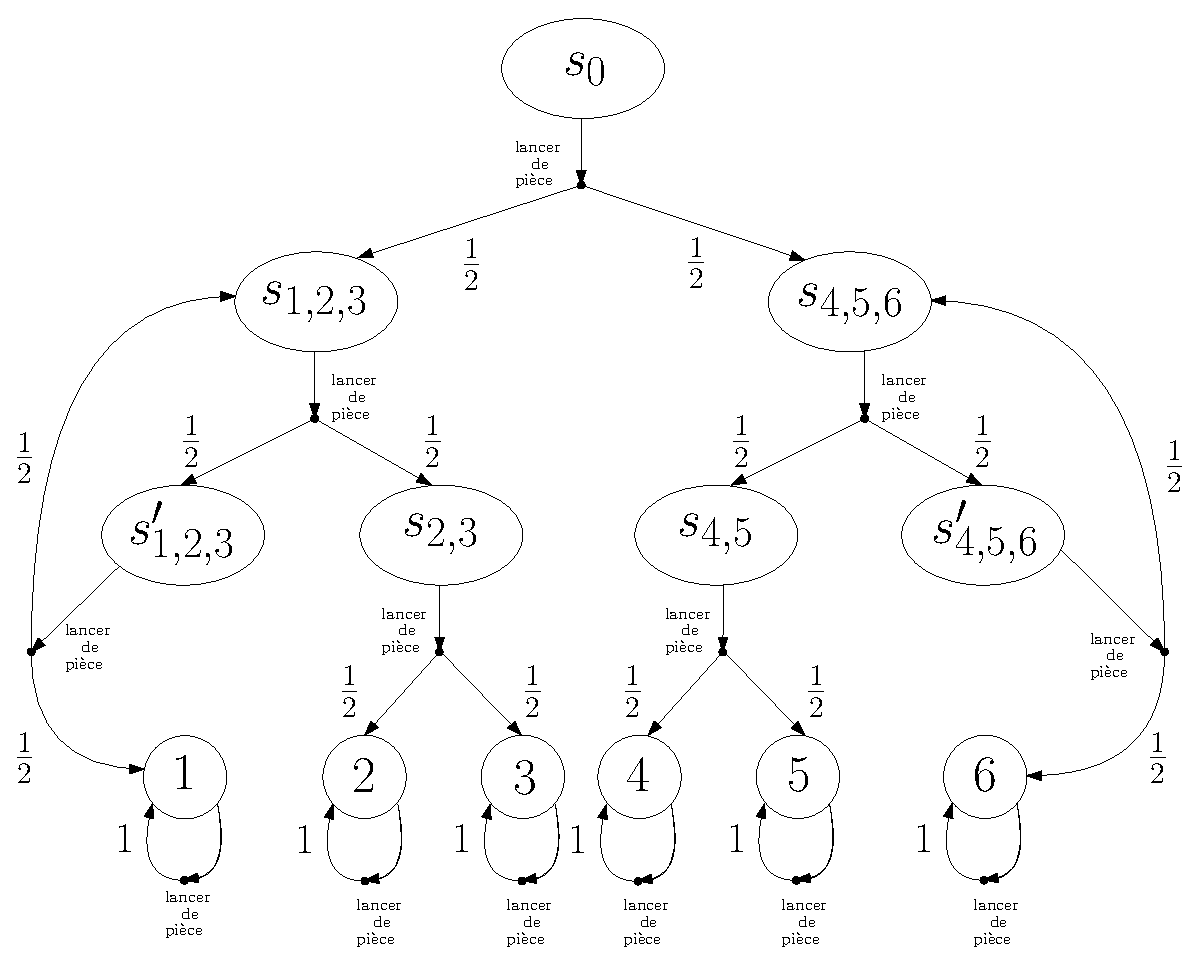
\includegraphics[scale=0.4]{figures/dieByaCoinPDM}
%		\end{minipage}
%		\caption{Par la propriété \ref{PDM=CM}, les deux systèmes sont équivalents.}
%		\label{PDM=CM-example}
%	\end{figure}
%\end{example}

\begin{remark}
	Soient $\mathcal{M} = (S, A, \Delta)$, un PDM et $\alpha_1, \alpha_2 \in A$,
	deux actions. Si pour tout état $s \in S$, les successeurs-$\alpha_1$ et
	successeurs-$\alpha_2$ de $s$ sont égaux et que pour chacun de ces successeurs
	$s'$, $\Delta(s, \alpha_1, s') = \Delta(s, \alpha_2, s')$, alors $\alpha_1 =
	\alpha_2$.
\end{remark}


\begin{definition}[\textbf{Graphe sous-jacent d'un processus décisionnel de Markov}]
	Un PDM $\mathcal{M} = (S, A, \Delta)$ induit un \textit{graphe sous-jacent} (orienté) $G^\mathcal{M} = (V, E)$ où :
	\begin{itemize}
		\renewcommand{\labelitemi}{\tiny $\bullet$}
		\item Comme dans une chaîne de Markov, l'ensemble des sommets $V$ du graphe correspond à l'ensemble des états du système. Par abus de langage, on dit que $V = S$ (\cf définition \ref{markov-underlying-graph}).
		\item $E$ est l'ensemble des arcs du graphe. On a que l'arc $(s, s') \in E$ \ssi il existe une action $\alpha \in A(s)$ telle que $\Delta(s, \alpha, s') > 0$.
	\end{itemize}
\end{definition}

\begin{propriete}
Tout PDM $\mathcal{M} = (S, A, \Delta)$ est fini ssi $S$ et $A$ sont finis. La taille de $\mathcal{M}$
correspond au nombre de triplets $(s, \alpha, s')$ tels que $\Delta(s, \alpha, s') > 0$. Soit $G^\mathcal{M} = (S, E)$, le graphe sous-jacent de $\mathcal{M}$. Par définition de $E$, on a
\[ |\mathcal{M}| = \mathcal{O}(|E| \, |A|) \]
\end{propriete}

En effet,
\begin{flalign*}
	|\mathcal{M}|
	&= | \{ (s, \alpha, s') \in S \times A \times S \; | \; \Delta(s, \alpha, s') > 0 \} |\\
	&= | \{ (s, \alpha, s') \in S \times A \times S \; | \; s' \in Succ(s, \alpha) \} |\\
	&= \sum_{s \in S} \sum_{\alpha \in A(s)} | Succ(s, \alpha) | \\
	&= \mathcal{O}\big(\sum_{s \in S} |A| \, |succ(s)| \big) \\
	&= \mathcal{O}(|E| \, |A|)
\end{flalign*}

\begin{example}[\textit{Graphe sous-jacent de l'agent évoluant dans un labyrinthe}]
	Reprenons le PDM $\mathcal{M}_{\text{maze}}$ de l'exemple \ref{maze-agent}.
	Le graphe sous-jacent $G^{\mathcal{M}_{\text{maze}}}$ est donné à la figure
	\ref{graphe-maze} et $|\mathcal{M}_{\text{maze}}| = 20$.

	\begin{figure}[H]
		\centering
		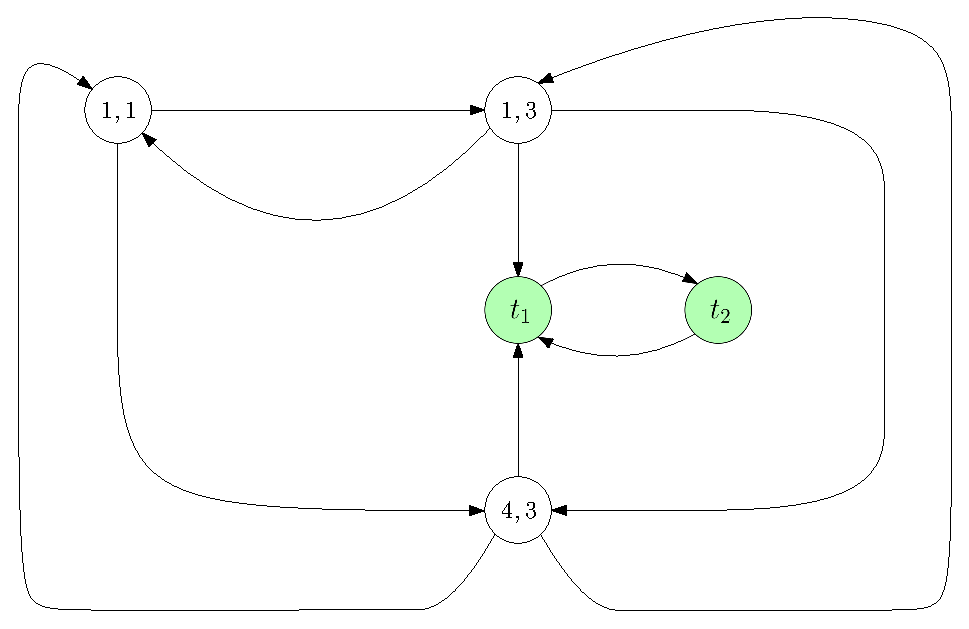
\includegraphics[scale=0.5]{figures/mazePDM-graphe}
		\caption{Graphe sous jacent du PDM $\mathcal{M}_{\text{maze}}$.}
		\label{graphe-maze}
	\end{figure}

\end{example}

%\begin{notation}
%	Les successeurs d'un état $s \in S$ sont dénotés par $Succ^*(s)$.
%	Cet ensemble est défini comme suit :
%	\[
%		Succ^*(s) = \{ s' \in S \; | \; \exists \alpha \in A(s), \; s' \in Succ(s, \alpha) \}
%	\]
%	ou encore de la façon suivante à l'aide du graphe sous-jacent
%	$G^\mathcal{M}$:
%	\[
%		Succ^*(s) = \{ s' \in S \; | \; s' \in succ(s) \text{ dans le graphe } G^\mathcal{M} \}
%	\]
%\end{notation}


\section{Chemins et Stratégies de PDM}

\begin{definition}[\textbf{Chemins dans un PDM}]
	Soit $\mathcal{M} = (S, A, \Delta)$, un PDM. Un chemin de $\mathcal{M}$ est une
	séquence infinie $s_0 \alpha_1 s_1 \alpha_2 s_2 \alpha_3 s_3 \dots \in (S \times A)^\omega$
	où $\forall i \in \mathbb{N}$, $\Delta(s_i, \alpha_{i+1}, s_{i+1}) > 0$. Dès lors, soit la relation de
	transition
	\[\rightarrow \; =  \{ (s, \alpha, s') \in S \times A \times S \; | \; \Delta(s, \alpha, s') > 0 \}, \,\]
	on définit un chemin $\pi$ de $\mathcal{M}$ comme suit :
	\[ \pi = s_0 \xrightarrow{\alpha_1} s_1 \xrightarrow{\alpha_2} s_2 \xrightarrow{\alpha_3} \dots \]
	Soit $s \in S$, un état de $\mathcal{M}$. $Paths(s)$ dénote l'ensemble des chemins
	infinis de $\mathcal{M}$ qui commencent en l'état $s$, et
	$Paths_{fin}(s)$ dénote l'ensemble des chemins finis de $\mathcal{M}$ commençant en l'état $s$.
	De la même façon, $Paths(\mathcal{M})$ dénote l'ensemble des chemins infinis de $\mathcal{M}$ et $Paths_{fin}(\mathcal{M})$ dénote l'ensemble des chemins finis de
	$\mathcal{M}$, avec $Paths(\mathcal{M}) = \bigcup_{s \in S} Paths(s)$ et
	$Paths_{fin}(\mathcal{M}) = \bigcup_{s \in S} Paths_{fin}(s)$.
\end{definition}

\begin{example}[\textit{Chemin d'un agent dans un labyrinthe}]
	Soit le PDM $\mathcal{M}_{\text{maze}}$ de l'exemple \ref{maze-agent}.
	Dans cette situation, un chemin de $\mathcal{M}_{\text{maze}}$ est en réalité
	un chemin infini possible pour l'agent lorsqu'il se déplace dans le labyrinthe.
	Le chemin
	\[\pi = (1,1) \xrightarrow{\downarrow} (4,3) \xrightarrow{\uparrow}
	\big(t_1 \xrightarrow{\rightarrow} t_2 \xrightarrow{\leftarrow} \big)^\omega \in Paths((1,1))\]
	est donc un chemin de $\mathcal{M}_{\text{maze}}$.

\end{example}

Ici, contrairement aux CM, les PDM ne sont pas équipés de $\sigma$-algèbre dû au
choix d'action
non-déterministe auquel le système est confronté à chaque étape (les choix ne suivent
donc pas une distribution de probabilité). \'Etudier les probabilités des chemins
d'un PDM est lié à l'étude de la résolution du non-déterminisme de ce PDM.
Le non-déterminisme peut être résolu grâce à une \textit{stratégie}.

\begin{definition}[\textbf{Histoire}]
	Soit $\mathcal{M} = (S, A, \Delta)$, un PDM. Une \textit{histoire} de $\mathcal{M}$
	est une séquence finie d'états $(s_0 \dots s_n) \in S^+$ telle que
	$\forall i \in \{1, \dots, n \}, \; \exists \alpha \in A(s_{i-1})$ telle que $\Delta(s_{i-1}, \alpha, s_i) > 0$.
	Une histoire d'un PDM est donc la succession d'états qui a amené l'état $s_0$ à l'état $s_n$ dans
	un chemin de $\mathcal{M}$.
\end{definition}

\begin{example}[\textit{Histoire d'un agent dans un labyrinthe}]
	Soit le PDM $\mathcal{M}_{\text{maze}} = (S, A, \Delta)$ de l'exemple \ref{maze-agent}.
	Une histoire de $\mathcal{M}_{\text{maze}}$ correspond, dans cette situation,
	à la succession de cases qui forme un chemin fini de l'agent lorsqu'il se deplace dans le
	labyrinthe. Ainsi,
	$
		h = \big( (1, 1) (4, 3) (1, 3) (1, 1) \big) \in S^+
	$
	est une histoire de $\mathcal{M}_{\text{maze}}$.
\end{example}

\begin{definition}[\textbf{Stratégie}]
	Soit $\mathcal{M} = (S, A, \Delta)$, un PDM. Une \textit{stratégie} pour $\mathcal{M}$
	est une fonction
	$\sigma : S^+ \rightarrow A$
	qui sélectionne pour toute histoire $h = (s_0 \dots s_n)$ de $\mathcal{M}$, une action réalisable, i.e., $\sigma(s_0 \dots s_n) = \alpha \in A(s_n)$.
	\\Le chemin $\pi = s_0 \xrightarrow{\alpha_1} s_1 \xrightarrow{\alpha_2} s_2 \xrightarrow{\alpha_3} \dots$
	est appelé $\sigma$-chemin ssi $\alpha_i = \sigma(s_0 \dots s_{i-1})$
	pour tout $i \in \mathbb{N}_0$.
\end{definition}
	Notons que les stratégies que l'on va utiliser dans ce document sont dites \textit{pures}, i.e., non-randomisée. Il existe également un autre type de
	stratégies que nous ne traiterons pas dans ce document dont l'ensemble des
	images est l'ensemble des distributions de probabilités sur $A$, i.e., les stratégies $\sigma$ telles que $\sigma: S^+ \rightarrow \mathcal{D}(A)$. \\

Supposons que $\sigma$ est une stratégie pour le PDM $\mathcal{M}$. Alors,
$\sigma$ résout le non-déterminisme lié aux choix des actions dans $\mathcal{M}$.
En effet, le comportement de $\mathcal{M}$ sous les décisions de $\sigma$
peut être formalisé sous la forme d'une CM $\mathcal{M}^{\sigma}$.

\begin{definition}[\textbf{CM d'un PDM induite par stratégie}]
Soit $\mathcal{M} = (S, A, \Delta)$, un PDM et $\sigma$, une stratégie pour
$\mathcal{M}$. La CM $\mathcal{M}^\sigma$ est donnée par
$ \mathcal{M}^\sigma = (S^+, \Delta_\sigma) $, où pour toute histoire
$h = s_0 s_1 \dots s_n$ de $\mathcal{M}$,
\[\Delta_\sigma(h, h . s_{n+1}) = \Delta(s_n, \sigma(h), s_{n+1}) \]
\end{definition}

Par construction, la CM $\mathcal{M}^{\sigma}$ va prendre la forme d'une forêt (1
arbre par état de $\mathcal{M}$), où chaque chemin de $\mathcal{M}^{\sigma}$
est en fait un $\sigma$-chemin de $\mathcal{M}$. \\

\begin{propriete}
	Soit $\mathcal{M}$, un PDM et $\sigma$, une stratégie pour $\mathcal{M}$.
	On peut faire correspondre, pour tout $\sigma$-chemin de $\mathcal{M}$,
	un chemin de $\mathcal{M}^\sigma$, la CM induite par $\sigma$.
	En effet, soit $\pi$, un $\sigma$-chemin de $\mathcal{M}$ tel que
	\[
		\pi = s_0 \xrightarrow{\alpha_1} s_1 \xrightarrow{\alpha_2} s_2 \xrightarrow{\alpha_3} \dots
\]
Le chemin $\pi^\sigma$ correspondant à $\pi$ dans $\mathcal{M}^\sigma$
est donné par
\[
	\pi^\sigma = \hat{\pi}_0\hat{\pi}_1\hat{\pi}_2\dots
\]
où $\hat{\pi}_n = s_0 \dots s_n$ est une histoire de $\mathcal{M}$ telle que cette
histoire est préfixe de $\pi$ et se termine en l'état $s_n$ après avoir parcouru
$n+1$ états.
Dès lors, on a que
\[
	\pi = s_0 \xrightarrow{\sigma(\hat{\pi}_0)} s_1 \xrightarrow{\sigma(\hat{\pi}_1)} s_2 \xrightarrow{\sigma(\hat{\pi}_2)} \dots
\]
\end{propriete}

\begin{example}[\textit{Stratégie naïve d'un agent pour résoudre un labyrinthe dans un milieu stochastique}] \label{example-strat-history}
	Soit le PDM $\mathcal{M}_{\text{maze}} = (S, A, \Delta)$ de l'exemple
	\ref{maze-agent}.	On va définir une stratégie naïve qui va permettre à l'agent d'atteindre les cases cibles.
	Pour ce faire, on suppose qu'il existe une fonction $\textit{étapes} : S \times \mathcal{P}(S) \rightarrow \mathbb{N} \cup \{ \infty \}$ qui calcule le
	nombre minimum d'étapes nécessaires afin de passer d'un état à un sous-ensemble d'états cibles, i.e., le nombre d'arcs empreintés dans le graphe sous-jacent $G^{\mathcal{M}_{\text{maze}}}$ pour atteindre le sous-ensemble (e.g., $\textit{étapes}\big((1,1), \{t_1, t_2\}\big) = 2$).
	On définit également les fonctions $dernier : S^+ \rightarrow S$ et $avant\text{-}dernier: S^+ \rightarrow S$
	qui calculent respectivement le dernier et avant-dernier état d'une
	histoire (par convention, soit $s \in S$, si $h = (s)$, alors $\textit{avant-dernier}(h) = s$). E.g., soit $h = \big((1, 1) (1, 3) (4, 3)\big)$, une histoire de
  $\mathcal{M}_{\text{maze}}$, $dernier(h) = (4, 3)$ et $avant\text{-}dernier(h) = (1,3)$. \par
	On définit $\sigma$ comme étant une stratégie qui va tenter de
	minimiser le nombre d'étapes pour atteindre
	les cases cibles. Cette stratégie va se servir de l'histoire afin d'éviter de choisir une action qui ferait repasser l'agent
	sur la case sur laquelle il était à l'étape précédente
	et ainsi d'éviter que l'agent "tourne en rond".
	En effet, si une telle action est
	choisie, alors la stratégie va de nouveau choisir l'action qui a amené
	l'agent sur la case actuelle, et cela risque donc de provoquer une "boucle"
	dans l'histoire.
%	Pour ce faire, on définit une nouvelle fonction
%	$suivant: S \times S \times A \rightarrow S$ de la façon suivante :
%
%	\[
%		suivant(s^*, s, \alpha) = \arg
%		\begin{cases}
%			\max_{s' \in Succ(s, \alpha)\setminus \{s^*\}} \Delta(s, \alpha, s') & \text{si $Succ(s, \alpha) \neq \{s^*\}$} \\
%			\max_{s' \in Succ(s, \alpha)} \Delta(s, \alpha, s') & \text{sinon}
%		\end{cases}
%	\]
%	\textit{(Note : $\arg \max_{s' \in Succ(s, \alpha, s')}$ correspond à l'état en lequel le système a le plus de chance d'évoluer quand l'action $\alpha$ est choisie, i.e., à la case vers laquelle l'agent a le plus de chance de se
%	diriger en choisissant la direction $\alpha$)}.\\
%	De cette façon, $suivant(\textit{avant-dernier}(s), dernier(s), \alpha)$ va retourner
%	la case vers laquelle l'agent a le plus de chance de se diriger si il
%	choisit l'action $\alpha$, sans considérer l'avant-dernière case sur laquelle
%	l'agent se situait

Pour ce faire, soient $h$, une histoire de
$\mathcal{M}_{\text{maze}}$, $T = \{t_1, t_2 \}$, les cases cibles, $s = dernier(h)$, $s^* =
\textit{avant-dernier}(h)$ et
\[A^{\text{excl}} =
\begin{cases}
	\{ \alpha^*\} \text{, avec } \alpha^* = \arg \max_{\alpha \in A(s)} \Delta(s, \alpha, s^*) & \text{si } |A(s)|
		\neq 1 \text{ et } \Delta(s,\alpha^*, s') \neq 0\\
	\varnothing & \text{sinon}
\end{cases},
\] le singleton contenant l'action qui a le plus de chance d'amener l'agent
vers l'avant-dernière case $s^*$ depuis la case où il se situe actuellement (à savoir $s$). On définit $\sigma$ comme suit :
\[
	\sigma(h) = \arg \min_{\alpha \in A(s) \setminus A^{\text{excl}}}
		\textit{étapes}\big(\max_{s' \in Succ(s, \alpha)} \Delta(s, \alpha, s'), \; T
		\big)
\]
\textit{(Note : $\arg \max_{s' \in Succ(s, \alpha)} \Delta(s, \alpha, s')$ correspond à l'état en lequel le système a le plus de chance d'évoluer quand l'action $\alpha$ est choisie, i.e., à la case vers laquelle l'agent a le plus de chance de se
diriger en choisissant la direction $\alpha$)}.\\

	\begin{figure}[H]
		\centering
		\captionsetup{justification=centering}
		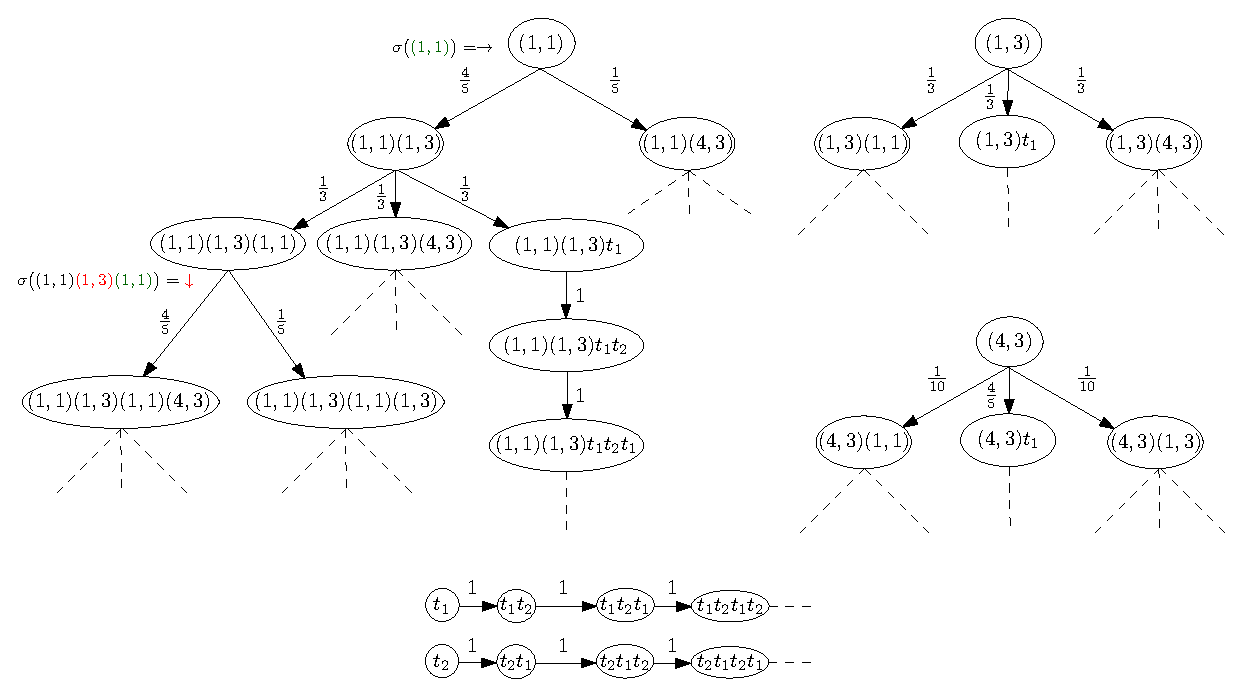
\includegraphics[scale=0.65]{figures/inductedMC}
		\caption{CM $\mathcal{M}^\sigma_{\text{maze}}$ induite par la
			stratégie $\sigma$.}
		\label{inducted-MC-strat1}
	\end{figure}
\end{example}

	De cette façon, \[\pi = (1, 1) \xrightarrow{\rightarrow} {\color{red}(1, 3)}
	\xrightarrow{\downarrow} (1, 1) {\color{red} \xrightarrow{\downarrow}} (4,
	3)\xrightarrow{\uparrow} \big(t_1 \xrightarrow{\rightarrow} t_2
	\xrightarrow{\leftarrow} \big)^\omega \] est un $\sigma$-chemin de
	$\mathcal{M}_{\text{maze}}$. En effet, d'abord, le système est en l'état
	$(1,1)$. La stratégie choisit l'action $\rightarrow$ car
	l'état $(1, 3)$ atteint $t_1$ en $1$ étape dans le graphe sous-jacent.
	Ensuite, elle choisit l'action $\downarrow$ pour accéder à la case $t_1$,
	mais cela échoue et renvoie l'agent dans la case $(1,1)$. La stratégie choisit
	alors l'action $\downarrow$ (et plus $\rightarrow$) car l'action effectuée
	lorsque le système se trouvait en $(1, 3)$ à l'étape précédente a renvoyé
	l'agent dans la case $(1, 1)$.
Cette stratégie induit une CM $\mathcal{M}^\sigma_{\text{maze}}$
	(cf. figure \ref{inducted-MC-strat1}).
		On peut faire correspondre le chemin $\pi$ de
	$\mathcal{M}_{\text{maze}}$ au chemin $\pi^\sigma$
	de $\mathcal{M}^\sigma_{\text{maze}}$, où
	\[
		\pi^\sigma = (1, 1) \; \; (1, 1) (1, 3) \; \;
		(1, 1) (1, 3) (1, 1) \; \;
		(1, 1) (1, 3) (1, 1) (4, 3) \; \;
		(1, 1) (1, 3) (1, 1) (4, 3) t_1 \; \; \dots
	\] \\

Comme la probabilité des chemins d'une CM est mesurable, toute stratégie
$\sigma$ d'un PDM $\mathcal{M}$ permet de mesurer les $\sigma$-chemins de ce PDM
en induisant une CM $\mathcal{M}^\sigma$ sur laquelle un espace probabiliste
est défini.
\begin{notation}
	%Soient $\mathcal{M} = (S, A, \Delta)$, un PDM, $\sigma$, une stratégie pour $\mathcal{M}$, $s \in S$, un état de $\mathcal{M}$ et
	Soient $\mathcal{M} = (S, A, \Delta)$, un PDM, $s \in S$, un état du système et
	$\sigma$, une stratégie définie pour $\mathcal{M}$.
	La mesure de probabilité induite par la stratégie $\sigma$ sur les
	$\sigma$-chemins de $Paths(s)$ est dénotée par $\pr^\sigma_s$.
\end{notation}

\begin{propriete}
Soient $\mathcal{M} = (S, A, \Delta)$, un PDM, $\sigma$, une stratégie définie pour
$\mathcal{M}$, $s \in S$, un état de $\mathcal{M}$ et $\pi = s_0 \alpha_1 s_1 \alpha_2 s_2 \alpha_3 \dots \in Paths(s)$ tel que $\pi$ est un $\sigma$-chemin. La
mesure de probabilité $\pr^\sigma_s(\{\pi\})$ est donc donnée par
\[
		\pr^\sigma_s(\{\pi\}) = \pr^{\mathcal{M}^\sigma}_{\hat{\pi}_0}(\{\pi^\sigma\})
\]
où $\hat{\pi}_0 = s_0 = s$
\end{propriete}
Les stratégies que l'on a étudiées jusqu'ici sont des stratégies à mémoire infinie, car les éléments du domaine de la stratégie (i.e., les histoires) sont infinis. De ce fait, la CM $\mathcal{M}^\sigma$ est infinie, et cela
même si $\mathcal{M}$ est finie%(à condition que $\mathcal{M}$ ne soit pas une CM)
. Intuitivement, l'état $s_0 s_1 \dots s_n$ de
$\mathcal{M}^\sigma$ représente la configuration du PDM $\mathcal{M}$ lorsque
le système est en $s_n$ et que son histoire est $s_0 \dots s_{n-1}$. Comme
$\sigma$ est dépendante de l'histoire du système, même si le système était en $s_{n-1}$ dans une autre configuration, i.e., si l'histoire du système était
différente, $\sigma$ pourrait sélectionner une action
différente (cf. exemple \ref{example-strat-history}).
%En effet, supposons au contraire que $\mathcal{M}^\sigma$ est finie.
%Soit $s_0 \in S$, un état de $\mathcal{M}$.
%Comme $\mathcal{M}^\sigma$ est une forêt, l'arbre ayant pour racine $s_0$ dans
%$\mathcal{M}^\sigma$ est également fini et possède donc des feuilles.
%Soit $s_0 \dots s_n$, une feuille de l'arbre de racine $s_0$. Par définition de
%$\sigma$ et par le fait que $A(s) \neq \varnothing$ pour tout $s \in S$, il existe une action $\alpha \in A(s_n)$ telle que
%$\sigma(s_0 \dots s_n) = \alpha$. Vu que $\alpha \in A(s_n)$, on a qu'il existe un état
%$s^*$ tel que $\Delta(s_n, \alpha, s^*) > 0$, et donc, il existe forcément le noeud (ou feuille) $s_0 \dots s_n s^*$ dans cet arbre. Comme l'histoire de ce noeud
%est $h =(s_0 \dots s_n)$, on a que le noeud $s_0 \dots s_n s^*$ est un
%fils de la feuille $s_0 \dots s_n$. La feuille $s_0 \dots s_n$ est donc un
%noeud. Il s'agit d'une contradiction. On a donc que le nombre d'arêtes dans
%le graphe sous-jacent de $\mathcal{M}^\sigma$ est infini, ce qui
%implique que la CM $\mathcal{M}^\sigma$ est inifinie.
%\begin{figure}[H]
%	\centering
%	\captionsetup{justification=centering}
%	\includegraphics[scale=0.64]{figures/CM-induite-arbre.eps}
%	\caption{$T_{s_0}^{\mathcal{M}^\sigma}$ est
%		l'arbre de la forêt formée par la CM
%		$\mathcal{M}^\sigma$ ayant pour racine $s_0$.}
%\end{figure}

Les \textit{stratégies à mémoire finies}
apportent une indépendance au niveau des histoires du PDM pour lequel la
stratégie est définie, ce qui permet d'induire des CM finies.

\begin{definition}[\textbf{Stratégie à mémoire finie}]
Soit $\mathcal{M} = (S, A, \Delta)$, un PDM. Une stratégie à mémoire finie
est un tuple $\sigma = (Q, \sigma_\alpha, \delta, \delta_0)$ formant un automate fini (plus précisément, une machine de Moore) où
\begin{itemize}
	\renewcommand{\labelitemi}{\tiny$\bullet$}
	\item $Q$ est un ensemble fini de modes,
	\item $\sigma_\alpha : Q \times S \rightarrow A$ est une fonction qui sélectionne pour tout état $s \in S$ une action $\alpha \in A(s)$ en fonction du mode $q \in Q$ dans lequel est
	l'automate,
	\item $\delta: Q \times S \rightarrow Q$ est la fonction de transition,
	\item $\delta_0 : S \rightarrow Q$ est la fonction qui choisit le mode initial de l'automate en fonction d'un état $s \in S$ avec lequel il va être initialisé.
\end{itemize}
\end{definition}

\begin{definition}[\textbf{Produit d'un PDM par une stratégie à mémoire finie}]
Soient $\mathcal{M} = (S, A, \Delta)$, un PDM et $\sigma = (Q, \sigma_\alpha, \delta, \delta_0)$, une stratégie à mémoire finie pour $\mathcal{M}$.
Le produit du PDM $\mathcal{M}$ par la stratégie $\sigma$ est donné par
\[ \mathcal{M} \times \sigma = \mathcal{M}^\sigma = (S \times Q, \Delta_\sigma) \]
où $\mathcal{M}^\sigma$ est la CM induite par la stratégie $\sigma$ et où
pour tout états $s, s' \in S$ et pour tout modes de la stratégie $q, q' \in Q$,
\[
	\Delta_\sigma\big((s, q), (s', q')\big) =
	\begin{cases}
	\Delta\big(s, \sigma_\alpha(q, s), s'\big) & \text{si } \delta(q, s) = q' \\
	0 & \text{sinon}
	\end{cases}
\]
\end{definition}

\begin{example}[\textit{Stratégie à mémoire finie sur un PDM simple}]
	Soit $\mathcal{M}_{\text{simple}} = (S, A, \Delta)$, un PDM (cf. figure \ref{finite_s1}). On suppose que le système est actuellement en l'état $s$.
	Soit $\sigma = (Q, \sigma_\alpha, \delta, \delta_0)$, une stratégie à mémoire finie (cf. figure \ref{finite_s2}).
	\begin{figure}[h]
		\centering
		\captionsetup{justification=centering}
		\begin{minipage}[t][][b]{0.45\textwidth}
		\centering
			\vspace{0.2\textwidth}
			\captionsetup{justification=centering}
			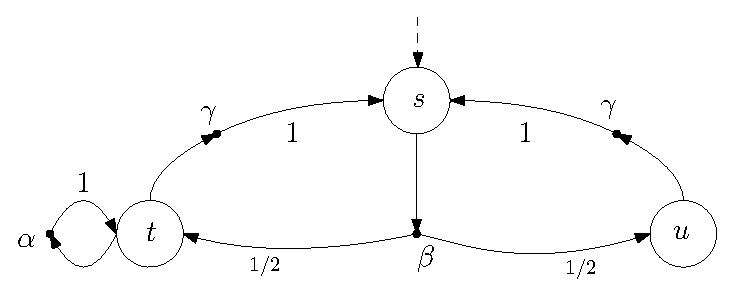
\includegraphics[scale=0.6]{figures/finite_scheduler1}
			\caption{PDM $\mathcal{M}_{\text{simple}}$.}
			\label{finite_s1}
		\end{minipage}
		\hspace{0.05\textwidth}
		\begin{minipage}[t][][b]{0.45\textwidth}
		\centering
			\includegraphics[scale=0.6]{figures/finite_scheduler2}
			\caption{Stratégie à mémoire finie $\sigma$.}
			\label{finite_s2}
		\end{minipage}
	\end{figure}
	On suppose que la stratégie est toujours initialisée dans le mode $m_1$, i.e., $\forall s \in S, \, \delta_0(s) = m_1$.
 La stratégie $\sigma$ est une stratégie qui consiste à atteindre l'état
 $t$ du système en passant au moins une fois par l'état $s$. Lorsqu'on
 applique la stratégie sur le le PDM $\mathcal{M}_{\text{simple}}$, son
 comportement est le suivant :
 \begin{enumerate}
 	\item Le PDM $\mathcal{M}_{\text{simple}}$ est actuellement en l'état $s$. On initialise la stratégie avec le mode $m_1$. Comme on se situe en l'état $s$, $\sigma_\alpha(m_1, s) = \beta$ est l'action retournée par la stratégie. Le mode de la stratégie est mis à jour par la fonction de transition : $\delta(m_1, s) = m_2$.
	\item Comme $\Delta(s, \beta, t) = \frac{1}{2}$ et $\Delta(s, \beta, u) = \frac{1}{2}$, le système a une chance sur deux d'évoluer en l'état $t$ et une chance sur deux d'évoluer en l'état $u$.
	On suppose ici que le système évolue en l'état $t$.
	\item Le PDM $\mathcal{M}_{\text{simple}}$ est actuellement en l'état $t$. Comme la stratégie est dans le mode $m_2$, $\sigma_\alpha(m_2, t) = \alpha$ est l'action retournée par la stratégie et comme $\delta(m_2, t) = m_2$, la stratégie reste dans le mode $m_2$.
	\item La $3^\text{ème}$ étape est répétée indéfiniement.
 \end{enumerate}
 Le $\sigma$-chemin de $\mathcal{M}$ formé par le comportement de la stratégie ci-dessus est le suivant :
 \[
 	\pi = s \xrightarrow{\beta} (t \xrightarrow{\alpha})^\omega \in Paths(s)
\]
La CM induite $\mathcal{M}^{\sigma}_{\text{simple}}$ est le produit du
PDM avec la stratégie $\sigma$ (cf. figure \ref{finite_s3}).
\begin{figure}[H]
\centering
\captionsetup{justification=centering}
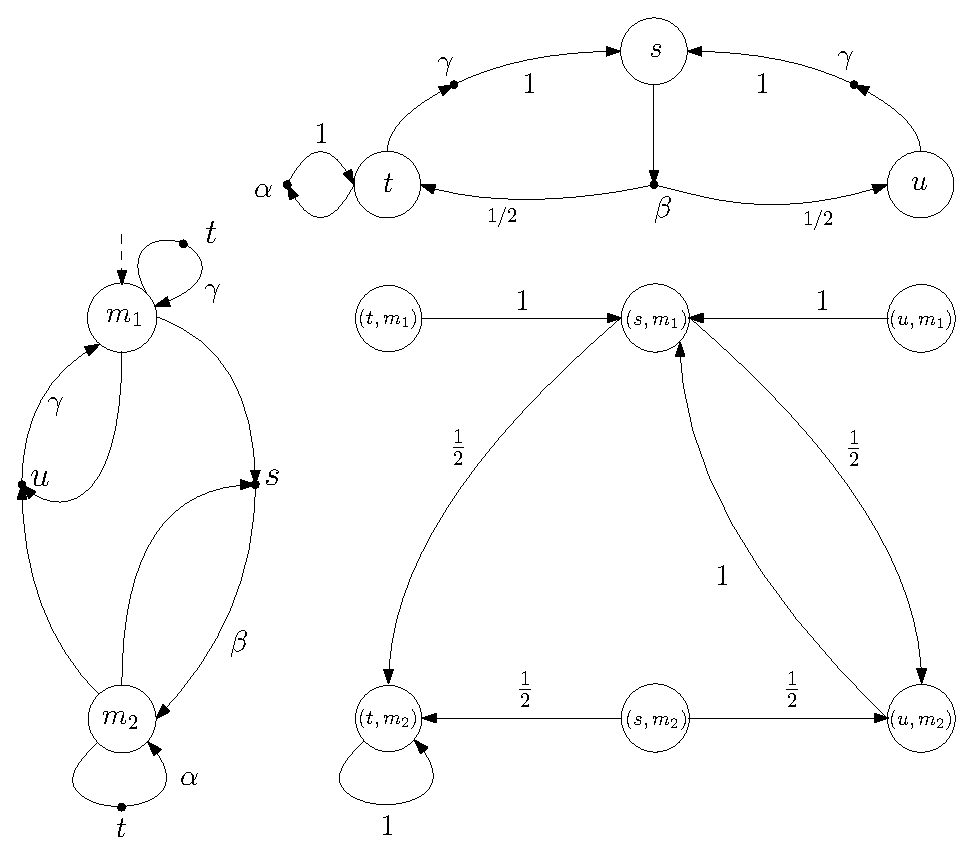
\includegraphics[scale=0.6]{figures/finite_scheduer}
	\caption{La chaine de Markov $\mathcal{M}^\sigma_{\text{simple}}$ induite par
	la stratégie $\sigma$ est en réalité le produit de $\sigma$ et $\mathcal{M}_\text{simple}$}
	\label{finite_s3}
\end{figure}

\end{example}

\begin{definition}[\textbf{Stratégie sans mémoire}]
	Soient $\mathcal{M} = (S, A, \Delta)$, un PDM et $\sigma$, une stratégie
	pour $\mathcal{M}$. La stratégie $\sigma$ est dite \textit{sans mémoire},
	ou encore \textit{simple}, si pour toutes histoires de $\mathcal{M}$ $(s_0 \dots s_n)$ et
	$(t_0 \dots t_m)$ telles que $s_n = t_m$,
	\[
		\sigma(s_0 \dots s_n) = \sigma(t_0 \dots t_m)
	\]
	Alors, $\sigma$ ne dépend pas de l'histoire complète du système, mais
	uniquement du dernier état dans lequel se trouve ce dernier. En effet,
	$\sigma$ va toujours sélectionner la même action pour différentes histoires données
	se terminant en un même état.
	Dès lors, $\sigma$ peut être vue comme étant une fonction
	\[
		\sigma: S \rightarrow A
	\]
	et on a donc
	$\sigma(s_n) = \sigma(s_0 \dots s_n) = \sigma(t_0 \dots t_m) = \sigma(t_m)$.
\end{definition}
\begin{propriete}
On peut associer toute stratégie sans mémoire $\sigma$ à une stratégie à mémoire finie $\sigma^* = (Q, \sigma^*_\alpha, \delta, \delta_0)$ ne possédant qu'un seul mode, i.e., telle que $|Q| = 1$. De ce fait, soit $q \in Q$, on a que
	$\forall s \in S, \; \sigma^*_\alpha(q, s) = \sigma(s)$,
	 $\delta(q, s) = q$ et
	 $\delta_0(s) = q$
\end{propriete}
\begin{example}[\textit{Stratégie sans mémoire pour résoudre un labyrinthe
dans un milieu stochastique}]
	Soit le PDM $\mathcal{M}_{\text{maze}} = (S, A, \Delta)$ de l'exemple
	\ref{maze-agent}.
	Comme pour l'exemple \ref{example-strat-history}, on va définir une stratégie
	$\sigma$ pour atteindre les cases cibles du labyrinthe, mais on ne va
	plus considérer les histoires du système.
	De ce fait, on va définir une stratégie plus simple qu'à l'exemple
	\ref{example-strat-history}, qui va naïvement tenter de minimiser le nombre
	d'étapes pour atteindre les cases cibles du labyrinthe.
	Soient $s \in S$, et $T = \{t_1, t_2 \}$, on définit $\sigma$ comme
	suit :
	\[
		\sigma(s) = \arg \min_{\alpha \in A(s)} \textit{étapes}\big(
			\arg \max_{s' \in Succ(s, \alpha)} \Delta(s, \alpha, s'), T\big)
	\]
	\textit{Note : on suppose qu'arbitrairement,
	$\sigma\big((1, 1)\big) = (1, 3)$ vu que $\textit{étapes}\big((1, 3), T\big)
	= \textit{étapes}\big((4, 3), T\big)$}.\\
	Dès lors, le chemin
	\[
		\pi = (1, 1) \xrightarrow{\rightarrow} (1, 3) \xrightarrow{\downarrow} (1, 1) \xrightarrow{\rightarrow} (1, 3) \xrightarrow{\downarrow}
		\big(t_1 \xrightarrow{\rightarrow} t_2
		\xrightarrow{\leftarrow} \big)^\omega
	\]
	est un $\sigma$-chemin de $\mathcal{M}_{\text{maze}}$. La stratégie
	induit une CM $\mathcal{M}_{\text{maze}}^\sigma$ (cf. figure
	\ref{CM-induite-strat-2}).
	Dès lors, on peut faire correpondre le chemin $\pi$ de
	$\mathcal{M}_{\text{maze}}$ avec le chemin $\pi^\sigma$
	de $\mathcal{M}_{\text{maze}}^\sigma$, avec
	\[
		\pi^\sigma = (1, 1) \; (1, 3) \; (1, 1) \; (1, 3) \; \big( t_1 \; t_2 \big)^\omega
	\]
	On peut donc mesurer la probabilité du chemin $\pi$ :
	\[
		\pr^\sigma_{(1, 1)}(\pi) =
		 \pr^{{M}_{\text{maze}}^\sigma}_{(1,1)}(\pi^\sigma)
		 = \Delta(\pi^\sigma) = \frac{4}{5} \cdot \frac{1}{3} \cdot \frac{4}{5} \cdot \frac{1}{3} \cdot 1^\omega = \frac{16}{225}
	\]
	\begin{figure}[H]
		\centering
		\captionsetup{justification=centering}
		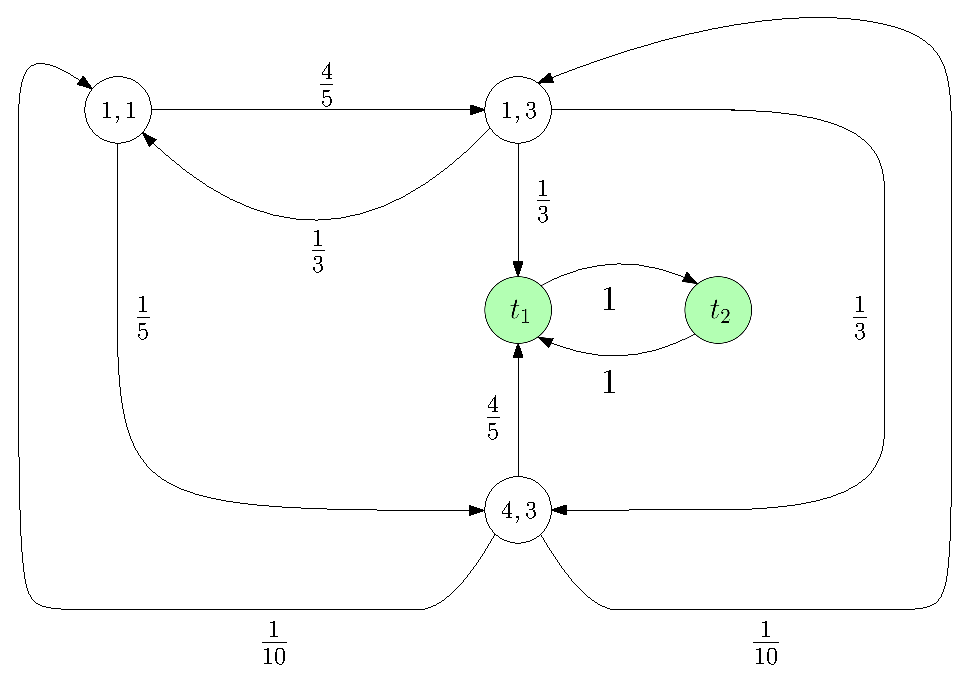
\includegraphics[scale=0.5]{figures/maze-PDM-inducted-S}
		\caption{CM $\mathcal{M}_{\text{maze}}^\sigma$ induite par la stratégie $\sigma$.}
		\label{CM-induite-strat-2}
	\end{figure}


\end{example}

\section{Problème d'accessibilité} \label{reachability-PDM}
Comme pour les CM, nous allons commencer par résoudre le problème d'accessibilité
dans un PDM, i.e., étudier la probabilité d'atteindre un sous-ensemble d'états cibles
du système, et cela pour chaque état. En effet, la résolution de ce problème est
fondamentale pour résoudre les problèmes que nous allons rencontrer par la suite.

\subsection{\'Enoncé du problème}
Soient $\mathcal{M} = (S, A, \Delta)$, un PDM et $T \subseteq S$, un sous-ensemble
d'états cibles. La mesure qui nous intéresse ici est la probabilité maximale
(ou minimale pour le problème dual) d'atteindre un état du sous-ensemble cible $T$
depuis un état du système $s \in S$. \\

Alors que dans les CMs on cherchait à connaitre la probabilité d'atteindre un
sous-ensemble d'états cibles depuis un état du système, les choix non-déterministes des PDMs entrainent
plusieurs espaces probabilistes et on cherche donc ici à connaitre celui qui va maximiser
la probabilité d'atteindre le sous-ensemble cible depuis un état du système.
Plus strictement, soit $s \in S$, l'état depuis lequel on veut atteindre le
sous-ensemble cible $T$,
\[
	\pr^{\max}_s(\Diamond T) = \sup_\sigma \pr^\sigma_s(\Diamond T)
\]

Ce supremum couvre toutes les stratégies définies pour $\mathcal{M}$, et leur nombre
est possiblement infini. \\

Le \textit{problème d'accessibilité} du PDM $\mathcal{M}$ consiste à calculer la valeur de
$\pr^{\max}(\Diamond T)$ pour tout état $s \in S$.

\subsection{Résolution du problème}
Ces probabilités maximales peuvent être calculées grâce à la résolution
d'un programme linéaire. On va également voir qu'il est inutile de considérer toutes
les stratégies possibles définies pour un PDM et qu'il suffit de ne considérer
que le sous-ensemble de stratégies sans mémoire. En effet, il existe une stratégie
sans mémoire qui maximise la probabilité d'atteindre $T$, et cela pour tout état
du PDM considéré.

\begin{theorem} \label{PDM-acc-thm}
	Soient $\mathcal{M} = (S, A, \Delta)$, un PDM, $s \in S$, un état de $\mathcal{M}$
	et $T \subseteq S$, un sous-ensemble d'états cibles. Le vecteur $(x_s)_{s \in S}$,
	avec $x_s = \pr^{\max}_s(\Diamond T)$ est l'unique solution du système d'équations
	suivant :
	\begin{enumerate}
		%\renewcommand{\labelitemi}{\tiny$\bullet$}
		\item Si $s$ est non-connexe à $T$ dans le graphe sous-jacent $G^\mathcal{M}$,
			alors $x_s = 0$.
		\item Si $s \in T$, alors $x_s = 1$.
		\item Si $s \not\in T$ et que la condition 1. n'est pas vérifiée, alors
			\[
				x_s = \max_{\alpha \in A(s)} \sum_{s' \in S} \Delta(s, \alpha, s') \cdot x_{s'}
			\]
	\end{enumerate}
\end{theorem}

\begin{figure}[H]
	\centering
	\captionsetup{justification=centering}
	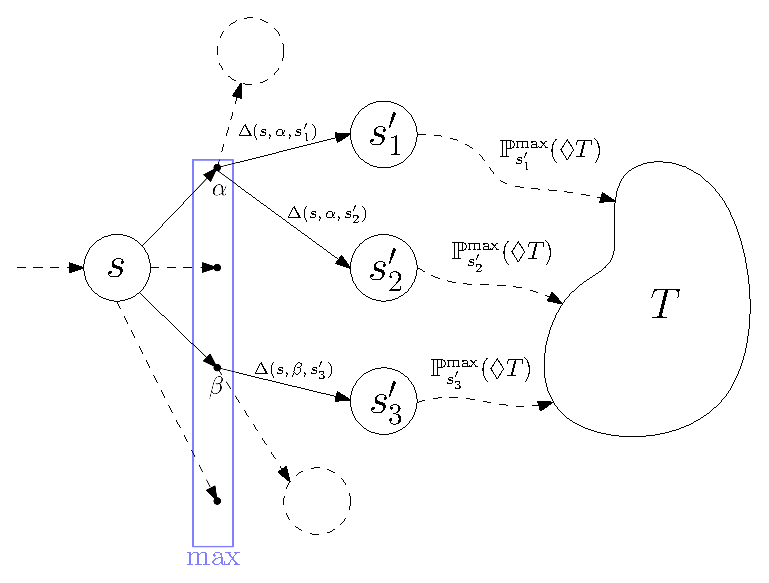
\includegraphics[scale=0.7]{figures/accessibilite-PDM-schema}
	\caption{Situation dans laquelle un état $s \not \in T$ et $s$ est connexe à
	$T$ dans le graphe sous-jacent d'un PDM.
	%L'action qui maximise la probabilité d'atteindre $T$ est choisie
	.}
	\label{PDM-acc-figure}
\end{figure}
	On suppose que le système est en l'état $s$ et que cet état $s$ satisfait la
	condition $3.$ du théorème \ref{PDM-acc-thm} (cf. figure
	\ref{PDM-acc-figure}). On suppose également que $x_{s'} =
	\pr_{s'}^{\max}(\Diamond T)$ pour tout $s' \neq s$. Afin de déterminer
	la valeur de $x_s$, on choisit l'action $\alpha$ qui maximise la probabilité
	d'atteindre $T$ depuis un état intermédiaire $s'$. Comme on connait déjà
	la probabilité maximale d'atteindre $T$ depuis ces états intermédiaires, il reste à
	connaitre la probabilité d'atteindre ces états intermédiaires depuis $s$.
	Celle-ci est donnée, pour tout successeur-$\alpha$ $s'$,
	par $\Delta(s, \alpha, s')$. La probabilité maximale que $s$ atteigne $T$
	en passant par l'état intermédiaire $s'$ est donc donnée par :
	\[\underbrace{\Delta(s, \alpha, s')}_{\text{probabilité de passer de $s$ à $s'$}} \cdot \underbrace{x_{s'}}_{\text{probabilité maximale pour que $s'$ atteigne $T$}}\]
	Il reste ensuite à faire la somme
	de ces probabilités pour tous les successeurs-$\alpha$ de $s$ pour obtenir
	$x_s$.

\begin{lemma}\label{strat-proof}
		Soient $\mathcal{M} = (S, A, \Delta)$, un PDM fini et $T \subseteq S$, un
		sous-ensemble d'états cibles. Il existe une stratégie sans mémoire
		$\sigma$ telle que, pour tout $s \in S$,
		\[
			\pr^\sigma_s(\Diamond T) = \pr^{\max}_s(\Diamond T)
		\]
\end{lemma}

\begin{proof}
	En effet, soit $x_s = \pr^{\max}_s(\Diamond T)$. On va construire une
	stratégie sans mémoire $\sigma$ telle que
	$\pr^\sigma_s(\Diamond T) = \pr^{\max}_s(\Diamond T)$.
	Pour ce faire, pour tout état $s$, on dénote par $A^{\max}(s)$ l'ensemble des
	actions $\alpha \in A(s)$ telles que
	$
		x_s = \sum_{s' \in S} \Delta(s, \alpha, s') \cdot x_{s'}
	$. Donc, vu que $x_s = \pr^{\max}_s(\Diamond T)$, les actions de $A^{\max}$
	maximisent la probabilité d'atteindre un état de $T$ depuis l'état $s$.
	\par Construire une stratégie qui choisit arbitrairement un état de l'ensemble
	$A^{\max}(s)$ n'est pas suffisant. En effet, prenons par exemple un état $s$
	tel que $A^{\max}(s) = \{\alpha, \beta\}$ où $\Delta(s, \beta, t) = 1$ pour un
	certain $t \in T$ et où choisir l'action $\alpha$ ne permet jamais au système
	d'atteindre $T$, i.e., $\Delta(s, \alpha, s) = 1$ (cf. figure
	\ref{accessibilite-preuve-strat}).

	\begin{figure}[H]
		\center
		\captionsetup{justification=centering}
		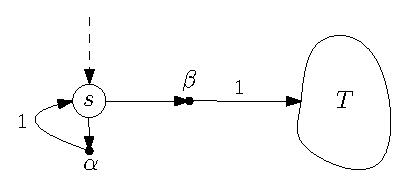
\includegraphics{figures/accessibilite-preuve}
		\caption{La stratégie $\sigma$ qui choisit toujours $\beta$ permet
			d'assurer au système de toujours atteindre un état de $T$ dans la CM
			$\mathcal{M}^\sigma$. Tandis que si la stratégie choisit
			toujours $\alpha$, alors $s$ n'atteindra jamais
			$T$ dans $\mathcal{M}^\sigma$.}
			\label{accessibilite-preuve-strat}
	\end{figure}

	Une sélection d'action est donc requise et cette dernière doit assurer
	l'accessibilité de $T$ dans la
	CM induite par la stratégie $\sigma$.
	On considère le PDM $\mathcal{M}^{\max}$ qui correspond au PDM $\mathcal{M}$
	où on a supprimé les actions $\beta \in A(s) \setminus A^{\max}(s)$ de $A(s)$
	pour tout état $s$ connexe à $T$ dans $G^\mathcal{M}$. Par définition, $\pr^{\max}_s$ n'est pas affectée par cette simplification de
	$\mathcal{M}$. \par
	Pour tout $s$ tel que $s$ est connexe à $T$ dans le graphe sous-jacent
	$G^{\mathcal{M}^{\max}}$, on dénote par $||s||$ la longueur du \textit{plus
	court chemin} de $s$ à n'importe quel état de $T$ dans
	$G^\mathcal{M^{\max}}$ (i.e., le nombre minimal d'arêtes empreintées par un chemin de $G^{\mathcal{M}^{\max}}$ pour atteindre $T$). Intuitivement, calculer la valeur de $||s||$ permet d'éviter que $\sigma$ choisisse des
	actions qui empêcheront d'atteindre $T$ (cf. $\alpha$ dans la figure
	\ref{accessibilite-preuve-strat}).
	\begin{itemize}
		\renewcommand{\labelitemi}{\tiny$\bullet$}
		\item $||s|| = 0$ ssi $s \in T$.
		\item Soit $n \in \mathbb{N}_0$. Par induction sur $n$, on définit
			$\sigma(s)$ pour tout état $s$ connexe à $T$ dans
			$G^{\mathcal{M^{\max}}}$ et tel que $||s|| = n$.
			La stratégie choisit une action $\sigma(s) \in A^{\max}(s)$ telle
			qu'il existe un successeur-$\sigma(s)$ $s'$ où $\Delta(s, \sigma(s), s') > 0$, avec $s'$ connexe à $T$ dans
			$G^{\mathcal{M}^{\max}}$ et $||s'|| = n - 1$. Une action $\sigma \in A(s)$ est choisie
			arbitrairement pour les états $s$ qui ne sont
			pas connexe à $T$ dans $G^{\mathcal{M}^{\max}}$.
	\end{itemize}
	On construit de cette façon la stratégie sans mémoire $\sigma$.
	Comme $\sigma$ est sans mémoire, la CM induite par stratégie
	$\mathcal{M}^\sigma$ est finie.
	On sait qu'il existe un système d'équations linéaires qui possède une solution
	unique $(y_s)_{s \in S}$, telle que $y_s = \pr^{\mathcal{M}^\sigma}_s(\Diamond T)$  pour tout état $s$ (cf. section \ref{accCM}) :
	\begin{enumerate}
		\item Si $s$ est non-connexe à $T$ dans $G^{\mathcal{M}^\sigma}$,
			alors $y_s = 0$.
		\item Si $s \in T$, alors $y_s = 1$.
		\item Si $s \not\in T$ est que la condition $1.$ n'est pas vérifiée, alors
			\[y_s = \sum_{s' \in S} \Delta(s, \sigma(s), s') \cdot y_{s'}\]
	\end{enumerate}
	Comme $x_s$ résout également ce système, on a
	\[
		\pr^\sigma_s(\Diamond T) = y_s = x_s = \pr^{\max}_s (\Diamond T)
	\]
\end{proof}

Il est possible de réécrire le système d'équations linéaires du théorème
\ref{PDM-acc-thm} sous forme d'un programme linéaire afin de calculer
$\pr^{\max}_s(\Diamond T)$ pour tout état $s$.

\begin{theorem} \label{LP-acc}
Soient $\mathcal{M} = (S, A, \Delta)$, un PDM fini et $T \subseteq S$, un
sous-ensemble d'états cibles. Le vecteur $(x_s)_{s \in S}$ avec
$x_s = \pr^{\max}_s(\Diamond T)$ est l'unique solution optimale du programme linéaire suivant :
\[
	\min \sum_{s \in S} x_s
\]
sous les contraintes suivantes :
\begin{flalign*}
	x_s &= 1 \quad &&\forall s \in T, \\
	x_s &= 0 \quad &&\forall s \not\in T \text{ tels que $s$ n'est pas connexe à $T$ dans $G^\mathcal{M}$}, \\
	x_s &\geq \sum_{s' \in S} \Delta(s, \alpha, s') \cdot x_{s'}
	\quad &&\forall \alpha \in A(s) \text{ et } \forall s \not \in T \text{ tels
		que $s$ est connexe à $T$ dans $G^\mathcal{M}$}. \\
	0 &\leq x_s \leq 1 && \forall s \in S
\end{flalign*}
\end{theorem}

Soient $(x_s)_{s \in S}$, la solution du système d'équations linéaires du
théorème \ref{PDM-acc-thm} et $(y_s)_{s \in S}$, une solution optimale
 du programme linéaire (dit PL) du théorème \ref{LP-acc}. \par
Tout d'abord, on remarque que les deux premières conditions sont équivalentes, dans le
système d'équations linéaires ainsi que dans le PL.
On a donc que $x_s$ satisfait toutes les contraintes du PL. En effet,
comme pour tout état $s \not\in T$ connexe à $T$ dans $G^\mathcal{M}$, $x_s = \max_{\alpha \in A(s)} \sum_{s' \in S} \Delta(s, \alpha, s') \cdot x_{s'}$
, on a forcément que $x_s \geq \sum_{s' \in S} \Delta(s, \alpha, s') \cdot x_{s'}$ pour tout
$\alpha \in A(s)$.
Comme $(y_s)_{s \in S}$ est une solution optimale du PL,
$\sum_{s \in S} x_s \geq \sum_{s \in S} y_s$. \par
%Ensuite, par le fait que $\sum_{s \in S} y_s$ est minimal, on a intuitivement que
%Ensuite, on a que
%\begin{flalign*}
%	x_s &= y_s = 1 \quad \forall s \in S \text{ tels que $s \in T$, } \\
%	x_s &= y_s = 0 \quad \forall s \in S \text{ tels que $s$ n'est pas connexe
%		à $T$ dans $G^\mathcal{M}$}, \\
%	x_s &= \max_{\alpha \in A(s)} \sum_{s' \in S} \Delta(s, \alpha, s') \cdot
%		x_{s'} \quad \forall s \in S \setminus T \text{ tels que $s$ est connexe à $T$ dans $G^\mathcal{M}$}\\
%	\text{et } y_s &\geq \sum_{s' \in S} \Delta(s, \alpha, s') \cdot y_{s'}
%	\quad \forall \alpha \in A(s), \; \forall s \in S \setminus T \text{ tels que $s$ est connexe à $T$ dans $G^\mathcal{M}$}.\\
%	\text{Donc, } y_s &\geq \max_{\alpha \in A(s)} \sum_{s' \in S} \Delta(s, \alpha, s') \cdot y_{s'} \quad \forall s \in S \setminus T
%	\text{ tels que $s$ est connexe à $T$ dans $G^\mathcal{M}$}.
%\end{flalign*}
%On en déduit que $\sum_{s \in S} x_s \leq \sum_{s \in S} y_s$ et donc que
%$\sum_{s \in S} x_s = \sum_{s \in S} y_s$. Cela signifie que $x_s$ est une
%solution optimale du PL. Finalement, on a
%\[
%	\sum_{s \in S}x_s = \sum_{s \in S} y_s
%\]
%avec
%\begin{flalign*}
%	x_s &= y_s = 1 \quad \forall s \in S \text{ tels que $s \in T$, } \\
%	x_s &= y_s = 0 \quad \forall s \in S \text{ tels que $s$ n'est pas connexe
%		à $T$ dans $G^\mathcal{M}$}, \\
%	x_s &= \max_{\alpha \in A(s)} \sum_{s' \in S} \Delta(s, \alpha, s') \cdot
%		x_{s'} \quad \forall s \in S \setminus T \text{ tels que $s$ est connexe à $T$ dans $G^\mathcal{M}$ et }\\
%	y_s &\geq \max_{\alpha \in A(s)} \sum_{s' \in S} \Delta(s, \alpha, s') \cdot y_{s'} \quad \forall s \in S \setminus T
%\text{ tels que $s$ est connexe à $T$ dans $G^\mathcal{M}$}.
%\end{flalign*}
%
%et donc, on a forcément que $x_s = y_s$ pour tout $s \in S$.
Ensuite, comme pour tout $s \not \in T$ connexe à $T$ dans $G^\mathcal{M}$,
$y_s \geq \sum_{s' \in S} \Delta(s, \alpha, s') \cdot y_{s'}$ pour tout $\alpha \in A(s)$ et
comme $\sum_{s \in S} y_s$ est minimale, on a intuitivement que
la contrainte est serrée avec
%$y_s = \sum_{s' \in S} \Delta(s, \alpha^*, s') \cdot y_{s'}$. En effet,
%cela est vrai avec $\alpha^* = \arg \max_{\alpha \in A(s)} \sum_{s' \in S} \Delta(s, \alpha, s') \cdot y_{s'} $. Donc, on a que \[
$y_s = \max_{\alpha \in A(s)} \sum_{s' \in S} \Delta(s, \alpha, s') \cdot y_{s'}$. Ceci est équivalent à la condition $3.$ du système d'équations
linéaires.
	Donc, $(y_s)_{s \in S}$ est solution du système d'équations linéaires. Comme
	cette solution est unique, $(x_s)_{s \in S} = (y_s)_{s \in S}$ et $(y_s)_{s
\in S}$ est unique.

\begin{corollaire}
	Soient $\mathcal{M} = (S, A, \Delta)$, un PDM fini, $T \subseteq S$, un
	sous-ensemble d'états cibles et $s \in S$, un état de $\mathcal{M}$,
	$\pr^{\max}_s(\Diamond T)$ peut être calculée en temps polynomial en la taille de $\mathcal{M}$.
\end{corollaire}

\begin{example}[\textit{Résolution du problème d'accessibilité dans un labyrinthe stochastique}]
	Soit $\mathcal{M}_{\text{maze}} = (S, A, \Delta)$, le PDM de l'exemple
	\ref{maze-agent}. On suppose que l'agent commence à se déplacer en haut à
	gauche du labyrinthe, i.e., depuis la case $(1, 1)$. On souhaite
	connaitre la probabilité maximale que l'agent atteigne les cases cibles $t_1$
	et $t_2$ depuis cette case $(1, 1)$, i.e.,
	$\pr^{\max}_{(1, 1)}(\Diamond \{t_1, t_2\})$. Pour ce faire, il faut résoudre
	le problème d'accessibilité pour le PDM $\mathcal{M}_{\text{maze}}$.
	On définit le programme linéaire suivant :
	\[
		\min x_{(1, 1)} + x_{(1, 3)} + x_{(4, 3)} + x_{t_1} + x_{t_2}
	\]
	sous les contraintes \\
 	\begin{equation*}
  \renewcommand{\arraystretch}{1.3}
  \begin{array}{ll}
		x_{(1, 1)} \geq \frac{4}{5} x_{(1, 3)} + \frac{1}{5} x_{(4, 3)}
			\quad & (\alpha = \rightarrow) \\
		x_{(1, 1)} \geq \frac{1}{5} x_{(1, 3)} + \frac{4}{5} x_{(4, 3)}
			\quad & (\alpha = \downarrow) \\
		x_{(1, 3)} \geq \frac{1}{3} x_{(1, 1)} + \frac{1}{3} x_{(4, 3)} + \frac{1}{3} x_{t_1}
			\quad & (\alpha = \downarrow) \\
		x_{(1, 3)} \geq \frac{9}{10} x_{(1, 1)} + \frac{1}{10}x_{t_1}
			\quad & (\alpha = \leftarrow) \\
		x_{(1, 3)} \geq \frac{9}{10} x_{(4, 3)} + \frac{1}{10}x_{t_1}
			\quad & (\alpha = \rightarrow)\\
		x_{(4, 3)} \geq \frac{1}{10} x_{(1, 1)} + \frac{1}{10} x_{(1, 3)} + \frac{4}{5}x_{t_1}
			\quad & (\alpha = \uparrow)\\
		x_{(4, 3)} \geq \frac{9}{10} x_{(1, 1)} + \frac{1}{10}x_{t_1}
			\quad & (\alpha = \leftarrow)\\
		x_{(4, 3)} \geq \frac{9}{10} x_{(1, 3)}
			\quad & (\alpha = \downarrow) \\
	%x_{t_1} \geq 1, \;
	%- x_{t_1} \geq -1, \;
	%x_{t_2} \geq 1, \;
	%- x_{t_2} \geq -1
		1 \geq x_{(1, 1)}, \; x_{(1, 3)}, \; x_{(4, 3)} \geq 0 \\
		x_{t_1} = x_{t_2} = 1
	\end{array}
 	\end{equation*}

Selon le théorème \ref{LP-acc}, il existe une solution unique $(x_s)_{s \in S}$
à ce PL tel que \[(x_s)_{s \in S} = \pr^{\max}_s (\Diamond \{t_1, t_2\})\]
On réécrit ce PL sous sa forme canonique :
%\begin{gather*}
%	\min_{x \in \mathbb{Q}^3} c^t x \\
%	\text{tel que} \quad Ax \geq b
%\end{gather*}
%	avec
\begin{gather*}
	\min_{(x_s)_{s \in S \setminus \{ t_1, t_2\} }}
		\begin{pmatrix}
			1 & 1 & 1
		\end{pmatrix}
		\begin{pmatrix}
			x_{(1, 1)} \\[0.3em]
			x_{(1, 3)} \\[0.3em]
			x_{(4, 3)}
		\end{pmatrix}
		\\
		\text{sous les contraintes} \quad
		\begin{pmatrix}
			1 & \frac{-4}{5} & \frac{-1}{5} \\[0.3em]
			1 & \frac{-1}{5} & \frac{-4}{5} \\[0.3em]
			\frac{-1}{3} & 1 & \frac{-1}{3} \\[0.3em]
			\frac{-9}{10} & 1 & 0 \\[0.3em]
			0 & 1 & \frac{-9}{10} \\[0.3em]
			\frac{-1}{10} & \frac{-1}{10} & 1 \\[0.3em]
			\frac{-9}{10} & 0 & 1 \\[0.3em]
			0 & \frac{-9}{10} & 1
		\end{pmatrix}
		\begin{pmatrix}
			x_{(1, 1)} \\[0.3em]
			x_{(1, 3)} \\[0.3em]
			x_{(4, 3)}
		\end{pmatrix}
		\; \geq \;
		\begin{pmatrix}
			0 \\[0.3em]
			0 \\[0.3em]
			\frac{1}{3} \\[0.3em]
			\frac{1}{10} \\[0.3em]
			\frac{1}{10} \\[0.3em]
			\frac{4}{5} \\[0.3em]
			\frac{1}{10} \\[0.3em]
			\frac{1}{10}
		\end{pmatrix} \\[0.3em]
		\text{ et tel que } 1 \geq x_{(1, 1)}, \; x_{(1, 3)}, \; x_{(4, 3)} \geq 0
\end{gather*}
Cela permet de résoudre le problème grâce à des algorithmes de résolution de
PL (e.g., par la méthode du simplexe).
Dans notre cas, on résout le problème à l'aide du module \verb|linprog|
de la bibliothèque \verb|scipy|, en \verb|python| avec la méthode du simplexe.
Dès lors, la solution de ce
système est donc $x_{(1, 1)} = x_{(1, 3)} = x_{(4, 3)} = x_{t_1} = x_{t_2} = 1$
(ce qui est logique, car tout sommet du graphe sous-jacent $G^{\mathcal{M}_{\text{maze}}}$
est connexe à $\{t_1, t_2 \}$).
\\
\end{example}

Certains problèmes nécessitent de savoir si un état $s \in S$ peut toujours
atteindre $T$, i.e., si $\pr^{\max}_s(\Diamond T) = 1$.
Bien que résoudre un PL où toutes les variables sont continues peut se faire
en temps polynomial, il n'est pas nécessaire de résoudre un PL pour déterminer
les états $s$ qui vérifient $\pr^{\max}_s(\Diamond T) = 1$.
En effet, cela peut être calculé à l'aide du graphe sous-jacent
$G^\mathcal{M}$ par un algorithme de parcours de graphe, polynomial en
$|\mathcal{M}|$. Dès lors, on peut diminuer le nombre de variables du PL, en
prétraitant le PDM pour déterminer les états $s \in S$ qui vérifient
$x_s = \pr^{\max}_s(\Diamond T) = 1$.

\section{Le problème du plus court chemin stochastique}
On va maintenant étudier des PDM enrichis de poids sur chacune de leurs
actions. En effet, chaque action aura maintenant un coût. Cela permet
d'apporter un contenu encore plus riche aux systèmes qui modélisent les
situations probabilistes. Grâce à de tels PDM, il est désormais possible de modéliser
des problèmes comme par exemple les jeux de hasard, où chaque action aura un coût (e.g., parier peut être vu comme une action) ou encore
modéliser des situations dans le domaine de la finance où tout investissement
a un coût et où les bénéfices (ou pertes) engendrés par cet investissement sont
incertains, etc.
\par
Lorsqu'on parle de coûts, une question naturelle apparait :
\textbf{Comment minimiser ces coûts ? Quelle stratégie employer ?} C'est
le sujet dont on va traiter dans cette section.
Le but de cette section est de définir des stratégies qui vont minimiser les
coûts des chemins de PDM pour atteindre des états cibles.
Le problème du plus court
chemin stochastique est naturellement en relation avec le problème des plus
courts chemins dans un graphe, car là aussi on cherche à atteindre des noeuds
avec un coût minimum et à déterminer quel chemin a le coût minimal. Le problème est néanmoins très différent dû aux
probabilités pour passer d'un état à un autre dans un PDM. Dès lors, on ne
peut pas définir une stratégie qui assure un coût minimal fixe, mais on peut
aborder deux problèmes :
\textit{le problème de l'espérance du plus court chemin stochastique} et
\textit{le problème des plus courts chemins stochastiques de taille limitée}.
Ces problèmes sont évidemment en relation avec les problèmes abordés au
chapitre précédent pour les CM, à savoir le problème de l'espérance du coût de l'accessibilité ainsi
que celui de l'accessibilité limitée par un coût.

\begin{definition}[\textbf{PDM pondéré}]
	Un PDM \textit{pondéré}, noté \textbf{PDMP}, est un tuple \\$\mathcal{M} = (S, A, \Delta, w)$, où
	\begin{itemize}
		\renewcommand{\labelitemi}{\tiny$\bullet$}
		\item $S, A, \Delta$ sont définis comme pour un PDM classique.
		\item $w : A \rightarrow \mathbb{N}_0$ est la fonction de coût qui
			associe un poids entier strictement positif à \textbf{chaque action}, i.e.,
			$\forall \alpha \in A,\; \exists n \in \mathbb{N}_0, \; w(\alpha) = n$.
	\end{itemize}
\end{definition}

\begin{remark}
	On représente un PDMP de la même façon qu'un PDM, mais chaque action $\alpha$
	est étiquetée par son coût.
	\begin{figure}[H]
	\centering
		\includegraphics{figures/PDMP-example}
	\end{figure}
\end{remark}

\begin{definition}[\textbf{CMP induite par stratégie}]
	Soient $\mathcal{M} = (S, A, \Delta, w)$, un PDMP et $\sigma$, une
	stratégie pour $\mathcal{M}$. La stratégie $\sigma$ induit une CMP
	$\mathcal{M}^\sigma = (S_\sigma, \Delta_\sigma, w_\sigma)$ telle que
	\begin{itemize}
		\renewcommand{\labelitemi}{\tiny$\bullet$}
		\item $S_\sigma$ et $\Delta_\sigma$ sont induits de la même
			façon que pour les CM classiques induites par stratégie,
		\item
			$\forall s, s' \in S_{\sigma}, \; \text{si} \;
			\Delta_{\sigma}(s, s') > 0, \; \text{alors} \; w_{\sigma}(s, s') = w\big(\sigma(s)\big)$.
	\end{itemize}
	%pour toute histoire $h = (s_0 \dots s_n) \in S^+$ avec $s_n = s \in S$, si $\exists s' \in S$ tel que $\Delta\big(s, \sigma(h), s'\big) > 0$, alors
	%$w_\sigma(h, h.s') = w\big(\sigma(h)\big)$.
\end{definition}


\begin{definition}[\textbf{Somme Tronquée d'un PDMP}]
	Soient $\mathcal{M} = (S, A, \Delta, w)$, un PDMP, $T \subseteq S$, un
	sous-ensemble d'états cibles et
	$\pi = s_0 \xrightarrow{\alpha_1} s_1 \xrightarrow{\alpha_2} s_2 \xrightarrow{\alpha_3} \dots \in Paths(\mathcal{M})$, un chemin dans
	$\mathcal{M}$. La somme tronquée du chemin $\pi$ dans $\mathcal{M}$ pour $T$
	est le coût total des actions nécessaires pour enchainer les états du chemin
	$\pi$ jusqu'à atteindre \textbf{pour la première fois} un des états cibles de
	$T$ (si le chemin n'atteint jamais un sommet de $T$, on dira que la somme
	tronquée est infinie). Plus strictement, soit $TS^T : Paths(\mathcal{M})
	\rightarrow \mathbb{N} \cup {\infty}$, la somme tronquée de $\pi$ pour atteindre $T$ dans
	$\mathcal{M}$. Celle-ci est définie par
	\[
		TS^T(\pi) =
		\begin{cases}
			\sum_{i = 1}^{n} w(\alpha_i) & \quad \text{si } \forall i \in \{0, \dots, n - 1\}, s_i \notin T \text{ et } s_n \in T \\
			\infty & \quad \text{si $ \nexists i \in \mathbb{N}$ tels que $s_i \in T$}
		\end{cases}
	\]
	\\
\end{definition}



\begin{example}[\textit{PDMP de l'agent se dirigeant dans un labyrinthe
stochastique}]\label{maze-pdmp}
	Soit $\mathcal{M}_{\text{maze}} = (S, A, \Delta)$, le PDM de l'exemple
	\ref{maze-agent}. On souhaite étudier la longueur des chemins de ce PDM,
	i.e., le nombre de cases que doit traverser l'agent pour atteindre les cases
	cibles $t_1$ et $t_2$. Pour ce faire, on va enrichir le système d'une
	fonction de coût $w : A \rightarrow \mathbb{N}_0$ qui va représenter le
	nombre de cases que l'agent traverse en effectuant une action. Afin
	de respecter le labyrinthe de l'exemple (cf. figure \ref{maze-figure}),
	il est utile d'introduire de nouveaux états et de nouvelles actions.
	Dès lors, soit $\mathcal{M}_{\text{maze}} = (S', A', \Delta, w)$, le PDMP
	représentant l'agent qui cherche à atteindre les cases $t_1$ et $t_2$ dans
	le labyrinthe stochastique (cf. figure \ref{maze-pdmp-figure}).
	On a $S' = S \cup \{(1, 2), (1, 2)', (2, 1), (2, 3), (1, 4), (4, 2), (5, 3) \}$ et
	$A' = A \cup \{\text{\rotatebox[origin=c]{180}{$\Lsh$},\rotatebox[origin=c]{90}{$\Rsh$},
	\rotatebox[origin=c]{180}{$\Rsh$} , \rotatebox[origin=c]{270}{$\Lsh$}}\}$.
On définit la fonction de coût comme suit : Soit $\alpha \in A$,
\[ w(\alpha) =
	\begin{cases}
		1 & \text{si } \alpha \in \{\leftarrow, \rightarrow, \uparrow, \downarrow\} \\
		4 & \text{si } \alpha \in \{
		\text{\rotatebox[origin=c]{180}{$\Lsh$},
		\rotatebox[origin=c]{90}{$\Rsh$}}\} \\
		10 & \text{si } \alpha \in \{ \rotatebox[origin=c]{180}{$\Rsh$} , \rotatebox[origin=c]{270}{$\Lsh$}\}
	\end{cases}
\]
ce qui va nous permettre de calculer le nombre de cases parcourues par l'agent.
	\begin{figure}[H]
		\centering
		\captionsetup{justification=centering}
		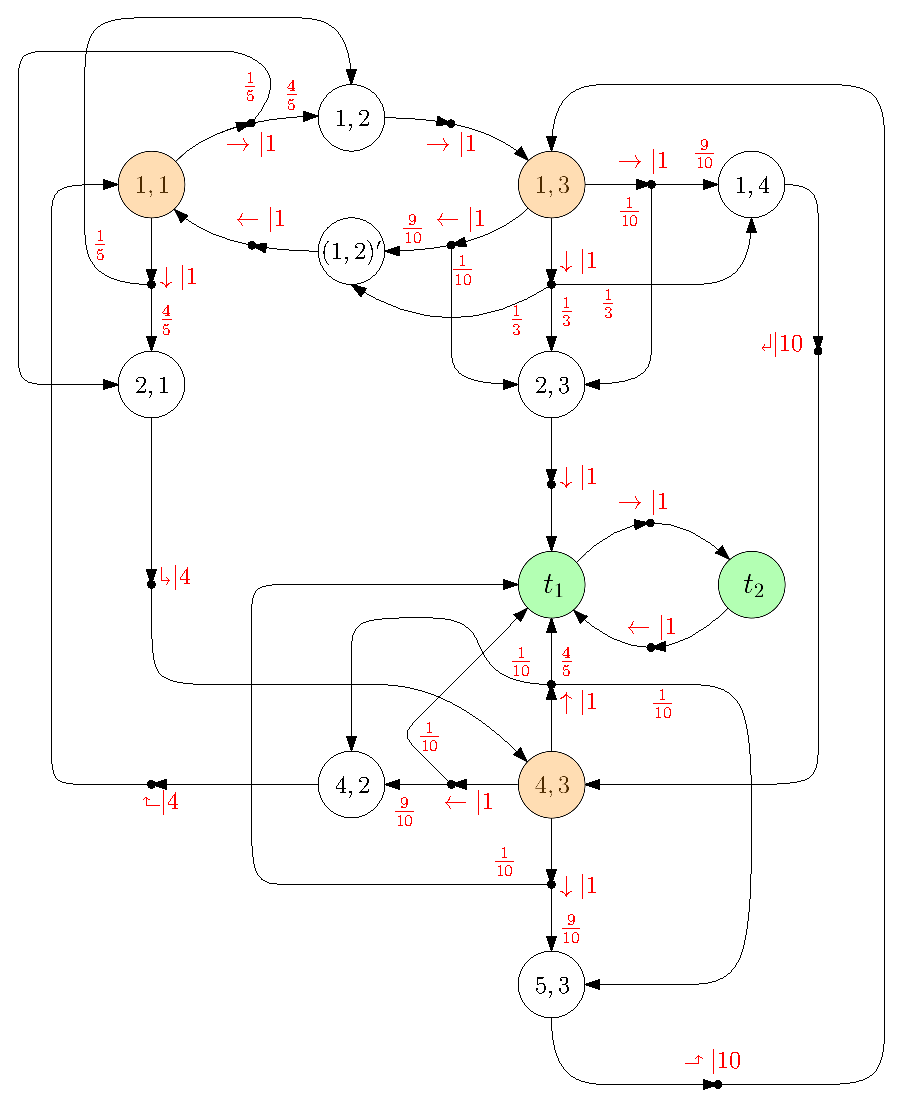
\includegraphics[scale=0.65]{figures/mazePDMP}
		\caption{PDMP représentant l'agent parcourant le labyrinthe stochastique de la figure
			\ref{maze-figure}. Les probabilités étiquetées sur les transitions pour lesquelles $\Delta(s, \alpha, s') = 1$ pour un certain $\alpha \in A(s)$
			sont omises sur la représentation du PDMP par souci de lisibilité.}
			\label{maze-pdmp-figure}
	\end{figure}
En effet, soit $\pi \in Paths((1, 1))$ tel que
\[\pi = (1, 1) \xrightarrow{\downarrow} (2, 1)
\xrightarrow{\text{\rotatebox[origin=c]{180}{$\Lsh$}}} (4, 3)
\xrightarrow{\uparrow} \big(t_1 \xrightarrow{\rightarrow} t_2
	\xrightarrow{\leftarrow} \big)^\omega \]
Le nombre de cases traversées par l'agent pour atteindre les cases cibles lorsqu'il empreinte ce chemin est
donné par la somme tronquée de ce chemin :
\begin{flalign*}
	TS^T(\pi)
	&= w(\downarrow) + w(\text{\rotatebox[origin=c]{180}{$\Lsh$}})
		+ w(\uparrow) \\
	&= 1 + 4 + 1 \\
	&= 6
\end{flalign*}
Ainsi, l'agent traverse 6 cases en empreintant ce chemin avant d'atteindre les
cases cibles $t_1$ ou $t_2$.
\end{example}


\subsection{Minimiser l'espérance de la longueur des chemins}\label{sspe}
	Le problème que l'on va traiter dans cette section est celui de
	\textit{l'espérance du plus court chemin stochastique} d'un PDMP.
	On s'intéresse donc au coût des chemins qui atteignent un sous-ensemble
	d'états cibles.
	Plus particulièrement, selon un état du système donné, le problème consiste
	à définir une stratégie qui va minimiser le coût espéré pour atteindre le
	sous-ensemble d'états cibles à partir de cet état.

	\begin{definition}[\textbf{L'espérance du plus court chemin stochastique}]
		Soient $\mathcal{M} = (S, A, \Delta, w)$, un PDMP, $T \subseteq S$, un
		sous-ensemble d'états cibles, $s \in S$, un état de $\mathcal{M}$ et
		$l \in \mathbb{Q}$, un seuil (longueur maximale).
		Le problème consiste à décider si il existe une
		stratégie $\sigma$ pour laquelle
		\[\mathbb{E}^{\sigma}_s (TS^T)\leq l\] où
		$\mathbb{E}^\sigma_s(TS^T) = \mathbb{E}^{\mathcal{M}^\sigma}_s(TS^T)$ est
		l'espérance du coût de l'accessibilité de l'état $s$ vers le sous ensemble $T$
		dans la CMP $\mathcal{M}^\sigma$ induite par la stratégie
		$\sigma$ (cf. section \ref{esp-access}).
	\end{definition}

	\begin{theorem}\label{esp-PDMP}
		Soient $\mathcal{M}=(S, A, \Delta, w)$, un PDMP fini et $T \subseteq S$,
		un sous-ensemble d'états cibles. Soient $S_{=1} = \{ s \in S \; | \; \pr^{\max}_s(\Diamond T) = 1\}$ et le vecteur $(x_s)_{s \in S}$. On définit le PL suivant :
		\[ \max \sum_{s \in S_{=1}} x_s \]
		sous les contraintes \\
	%	\begin{equation*}
	%  \renewcommand{\arraystretch}{1.3}
	%  \begin{array}{ll}
	%		x_s = \infty \quad
	%	\end{array}
	%\end{equation*}
	\begin{flalign*}
		x_s &= 0 && \forall s \in T \\
		x_s &= \infty && \text{$\forall s \in S$ tel que $\pr^{\max}_s(\Diamond T) < 1$} \\
		x_s &\leq w(\alpha) + \sum_{s' \in S \setminus T} \Delta(s, \alpha, s')
			\cdot x_{s'} && \forall \alpha \in A(s) \text{ et } \forall s \in S \setminus T \text{ tel que } \pr^{\max}_s(\Diamond T) = 1
	\end{flalign*}
	Ce PL a une solution optimale unique $(v_s)_{s \in S}$.
	On peut ensuite construire une stratégie sans mémoire optimale
	\[
		\sigma(s) = \arg \min_{\alpha \in A(s)} \bigg( w(\alpha) +
			\sum_{s' \in S \setminus T} \Delta(s, \alpha, s') \cdot v_{s'} \bigg)
	\]
	telle que
	\[
		 \mathbb{E}^\sigma_s(TS^T) = \min_\sigma \mathbb{E}^\sigma_s(TS^T)
	\]
	i.e., $\sigma$ minimise $\mathbb{E}^\sigma_s(TS^T)$. Dès lors,
	$v_s = \mathbb{E}^\sigma_s(TS^T)$ pour tout état $s \in S$.
	\end{theorem}
	\begin{remark}Soit $A^{\min}(s) = \arg \min_{\alpha \in A(s)} w(\alpha) +
			\sum_{s' \in S \setminus T} \Delta(s, \alpha, s') \cdot v_{s'} $.
			Le scénario dans lequel $|A^{\min}(s)| > 1$ ne pose pas de problème
			(cf. figure \ref{accessibilite-preuve-strat}) car $w : A \rightarrow
			\mathbb{N}_0$, i.e., la fonction de poids va toujours associer un coût
			$>0$, ce qui permet d'éviter de choisir des actions qui bloqueraient le
			système. Cependant, dans le cas où la fonction de poids permet d'associer
			un coût nul à une action, il est nécessaire de définir une stratégie
			d'une façon similaire à la démonstration du lemme \ref{strat-proof}.
	\end{remark}

	%Par le système d'équations linéaires défini dans la section
	%\ref{pb-esp-cout-acc} pour calculer l'espérance du coût de l'accessibilité
	%de toute CM à un sous ensemble d'états du système, et par la stratégie sans
	%mémoire optimale $\sigma$ définie ci-dessus, on a avec $\alpha = \sigma(s)$ :

	Intuitivement, le fait que $\sum_{s \in S} v_s$ est maximal
	mène au fait que la $3^e$ contrainte du PL est serrée avec
	\[ v_s = \min_{\alpha \in A(s)} \bigg( w(\alpha) + \sum_{s' \in S \setminus T} \Delta(s, \alpha, s') \cdot v_{s'} \bigg) \]
	Par la stratégie sans mémoire optimale $\sigma$ définie ci-dessus, on
	va montrer que la solution du PL est également la solution du système d'équations linéaires qui résout le problème d'espérance du coût de l'accessibilité de $\mathcal{M}^\sigma$
 (cf. le système d'équations linéaires défini à la section
\ref{pb-esp-cout-acc}).
	%avec $\alpha = \sigma(s)$ pour tout $s \in S \setminus T$
	\begin{enumerate}
\item Vu qu'on fixe $x_s$ à 0 pour tout $s \in T$, on a bien que $ (\mathbb{E}^\sigma_{t})_{t \in T}(TS^T) = 0$.
\item Fixer $x_s$ à $\infty$ pour tout $s \in S$ tel que $\pr^{\max}_s (\Diamond T) < 1$
permet d'assurer que
$\mathbb{E}_s^\sigma(TS^T) = \infty$ pour tout $s$ tel que $\pr^{\sigma}_s (\Diamond T) < 1$. En effet, \[\pr^{\sigma}_s (\Diamond T) < 1 \implies \pr^{\max}_s (\Diamond T)< 1\]
Afin de s'en convaincre, on prend la contraposée de cette implication, i.e.,\\
$\pr_s^{\max}(\Diamond T) = 1 \implies \pr_s^{\sigma}(\Diamond T) = 1$.
Cela est vrai. On suppose que $\pr_s^{\max}(\Diamond T) = 1$. Cela signifie
par le lemme \ref{strat-proof} qu'il existe une stratégie sans mémoire
$\sigma^*$ telle que $\pr_s^{\sigma^*}(\Diamond T) =
\pr^{\max}_s(\Diamond T) = 1$. Cela implique forcément que
$\pr^{\sigma}_s(\Diamond T) = 1$, car sinon, on aurait que
$\mathbb{E}^{\sigma^*}_s (TS^T) < \mathbb{E}^\sigma_s(TS^T) =
\infty$, ce qui est faux par définition de $\sigma$
($\sigma$ minimise $\mathbb{E}^\sigma_s(TS^T)$). Vu qu'on a fixé $x_s$ à $\infty$ pour tout $s \in S$ tel que $\pr^{\max}_s(\Diamond T) < 1$, et vu qu'on vient de prouver que $\pr^{\sigma}_s(\Diamond T) < 1 \implies \pr^{\max}_s(\Diamond T)
< 1$, on a bien que $v_s = \mathbb{E}_s^\sigma (TS^T)= \infty$ quand $\pr^{\sigma}_s
(\Diamond T) < 1$.


%\item Fixer $x_s$ à $\infty$ pour tout $s \in S$ tels que
%$\pr^{\max}_s(\Diamond T) < 1$ revient à fixer
%$\mathbb{E}^\sigma_s(TS^T)$ à $\infty$ quand $\pr_s^\sigma(\Diamond T)$ < 1,
%avec $\sigma$, la stratégie définie au théorème \ref{esp-PDMP}. En
%effet, pour rappel,
%\[
%	\pr_s^{\max}(\Diamond T) = 1 \iff \sup_{\sigma} \;
%	\pr_s^\sigma(\Diamond T) = 1
%\]
%Donc, on a que
%\[\pr_s^{\max}(\Diamond T) < 1 \iff \sup_{\sigma} \;
%\pr_s^\sigma(\Diamond T) < 1\]
%%i.e., si la probabilité d'accéder à $
%%T$ depuis $s$ est inférieure à $1$, aucune stratégie ne permet d'assurer
%%à $s$ d'accéder au sous-ensemble $T$ avec une probabilité de 1.
%Par le lemme \ref{strat-proof}, il existe une stratégie sans mémoire
%$\sigma^*$ telle
%que $\pr_s^{\max} = \pr_s^{\sigma^*}$. Supposons que
%\begin{itemize}
%\renewcommand{\labelitemi}{\tiny$\bullet$}
%\item Si $\pr_s^{\max}(\Diamond T) = 1$, alors on a forcément qu'il
%existe une stratégie $\sigma^*$ sans mémoire (cf. lemme
%\ref{strat-proof}) telle que
%$\pr_s^{\sigma^*}(\Diamond T) = 1$ et qui choisit une action
%$\alpha^* \in A(s)$ pour tout $s \in S$ qui a un coût minimal et qui permet d'accéder à $T$ avec une probabilité de $1$.
%Vu que $\sigma^*$ est sans mémoire, (cf. lemme \ref{strat-proof}),
%on a que $\exists \alpha^* \in A^{\max}(s')$ avec un coût minimal pour tout
%$s' \in S$
%qui permet d'accéder à $T$ avec une
%probabilité de 1
%($A^{\max}(s')$ est l'ensemble des
%actions disponibles de $s'$ qui maximisent la probabilité d'atteindre $T$, et donc ici, l'ensemble des actions disponibles de $s'$ qui permettent d'accéder à $T$ avec une probabilité de $1$).
%C'est donc cette action qui va être choisie par la stratégie $\sigma$
%définie au
%théorème \ref{esp-PDMP}. En effet, si $\sigma$ choisit une action qui
%ne figure pas parmis les actions qui permettent d'accéder à $T$ avec une probabilité de $1$, alors l'éspérance est infinie par définition de l'éspérance du coût de
%l'accessibilité dans une CM.
%De ce fait, on a que
%$\pr^{\sigma}_s(\Diamond T) =
%\pr^{\sigma^*}_s (\Diamond T)$
%\end{itemize}
%Cela mène au fait que $\pr^\sigma_s(\Diamond T) < 1 \implies \pr^{\max}_s(\Diamond T) < 1$, donc on a bien fixé
%les espérances des états $s$ pour lesquels $\pr^\sigma_s(\Diamond T) < 1$ à $\infty$.
	\item Pour tous les autres états $s \in S \setminus T$ :
	\begin{flalign*}
		\mathbb{E}_s^\sigma (TS^T)
		&= \min_{\alpha \in A(s)} \bigg( w(\alpha) + \sum_{s' \in S \setminus T}
			\Delta (s,
			\alpha, s') \cdot \mathbb{E}_{s'}^\sigma(TS^T) \bigg) \\
		&= \min_{\alpha \in A(s)} \bigg( w(\alpha) + \sum_{s' \in S}
			\Delta (s,
			\alpha, s') \cdot \mathbb{E}_{s'}^\sigma(TS^T) \bigg)
			\tag{\textit{\footnotesize avec $(\mathbb{E}_{t}^\sigma)_{t \in T}(TS^T) = 0$}}\\
		&= \min_{\alpha \in A(s)} \bigg( w(\alpha) + \sum_{s' \in Succ(s, \alpha)}
			\Delta (s,
			\alpha, s') \cdot \mathbb{E}_{s'}^\sigma(TS^T) \bigg)
			\tag{\textit{\footnotesize car $\Delta(s, \alpha, s') = 0$ pour tout
			$s' \not \in Succ(s, \alpha)$}}\\
		&= w(\alpha^*) + \sum_{s' \in Succ (s, \alpha^*)}
			\Delta (s,
			\alpha^*, s') \cdot \mathbb{E}_{s'}^\sigma(TS^T)
			\tag{\textit{\footnotesize par définition de $\sigma$, avec $\alpha^* = \sigma(s)$}}\\
		&= w( \alpha^*) \cdot \sum_{s' \in S} \Delta(s,
			\alpha^*, s') + \sum_{s' \in Succ (s, \alpha^*)}
			\Delta (s,
			\alpha^*, s') \cdot \mathbb{E}_{s'}^\sigma(TS^T) \tag{\textit{\footnotesize car $\Delta_{s, \alpha^*}$ est une distribution de probabilité sur $S$}}
			\\
		&= \sum_{s' \in Succ (s, \alpha^*)} \Delta(s,
			\alpha^*, s') \cdot w( \alpha^*) + \sum_{s' \in Succ (s, \alpha^*)}
			\Delta (s,
			\alpha^*, s') \cdot \mathbb{E}_{s'}^\sigma(TS^T) %\tag{\textit{\footnotesize par définition des CMP induites par stratégie}}
			\\
		&=\sum_{s' \in Succ (s, \alpha^*)} \Delta(s,
			\alpha^*, s') \cdot \big( w ( \alpha^* ) +
			\mathbb{E}_{s'}^\sigma(TS^T) \big) \\
		&=\sum_{s' \in succ(s)} \Delta_\sigma(s,s') \cdot \big( w_\sigma ( s, s' ) +
			\mathbb{E}_{s'}^\sigma(TS^T) \big)
	\end{flalign*}
\end{enumerate}

Par 1., 2. et 3., la solution du PL respecte bien la définition de l'espérance
du coût de l'accessibilité de la CMP induite par la stratégie $\sigma$.
\begin{corollaire}
	La stratégie sans mémoire optimale qui résout le problème de l'espérance du plus court chemin stochastique pour un PDM $\mathcal{M}$ peut être construite en temps polynomial en la taille de $\mathcal{M}$.
\end{corollaire}

\begin{example}[\textit{Espérance du plus court chemin de l'agent dans le
	labyrinthe stochastique}]\label{sspe-example}
	Soient $\mathcal{M}_{\text{maze}} = (S, A, \Delta, w)$, le PDMP de l'exemple
	\ref{maze-pdmp} représentant l'agent qui se déplace de la labyrinthe de la
	figure \ref{maze-figure} et $T = \{ t_1, t_2 \}$, les cases cibles
	de ce labyrinthe. On suppose que l'agent se situe dans la case $(1, 1)$
	et se déplace vers les cases $t_1$ ou $t_2$. Comme le labyrinthe est
	stochastique, on souhaite connaitre l'espérance du plus court chemin stochastique pour
	atteindre les cases $t_1$ ou $t_2$ depuis la case $(1, 1)$ et déterminer si il existe une stratégie qui résout ce problème et qui assure une espérance de la longueur du chemin inférieure à 10. Pour ce faire, on
	définit le PL suivant (par le théorème \ref{esp-PDMP}) :
\[
	\max_{s \in S \setminus T}
		x_{(1, 1)} + x_{(1, 2)} + x_{(1, 2)'} + x_{(1, 3)} + x_{(1, 4)}
		+ x_{(2, 1)} + x_{(2, 3)} + x_{(4, 2)} + x_{(4, 3)} + x_{(5, 3)}
\]
sous les contraintes
\footnotesize
	\[
  \renewcommand{\arraystretch}{1.3}
  \begin{array}{ll}
		x_{(1, 1)} &\leq w(\rightarrow) + \frac{4}{5} x_{(1, 2)} + \frac{1}{5}
			x_{(2, 1)} \\
		x_{(1, 1)} &\leq w(\downarrow) + \frac{1}{5} x_{(1, 2)} + \frac{4}{5}
			x_{(2, 1)} \\
		x_{(1, 3)} &\leq w(\downarrow) + \frac{1}{3} x_{(1, 2)'} + \frac{1}{3}
		x_{(1, 4)} + \frac{1}{3} x_{(2, 3)} \\
		x_{(1, 3)} &\leq w(\leftarrow) + \frac{9}{10} x_{(1, 2)'} +
			\frac{1}{10} x_{2, 3}\\
		x_{(1, 3)} &\leq w(\rightarrow) + \frac{9}{10} x_{(1, 4)} +
			\frac{1}{10} x_{2, 3}\\
		x_{(4, 3)} &\leq w(\uparrow) + \frac{1}{10} x_{(4, 2)} + \frac{1}{10}
			x_{(5, 3)} \\
		x_{(4, 3)} &\leq w(\leftarrow) + \frac{9}{10} x_{(4, 2)} \\
		x_{(4, 3)} &\leq w(\downarrow) + \frac{9}{10} x_{(5, 3)} \\
		x_{(1, 2)} &\leq w(\rightarrow) + x_{(1, 3)} \\
		x_{(1, 2)'} &\leq w(\leftarrow) + x_{(1, 1)} \\
		x_{(1, 4)} &\leq w(\text{\rotatebox[origin=c]{180}{$\Rsh$}}) + x_{(4, 3)} \\
		x_{(2, 1)} &\leq w(\text{\rotatebox[origin=c]{180}{$\Lsh$}})
		 	+ x_{(4, 3)} \\
		x_{(2, 3)} &\leq w(\downarrow) \\
		x_{(4, 2)} &\leq w(\text{\rotatebox[origin=c]{90}{$\Rsh$}})
			+ x_{(1, 1)} \\
		x_{(5, 3)} &\leq w(\text{\rotatebox[origin=c]{270}{$\Lsh$}})
			+ x_{(1, 3)}
	\end{array}
	\quad \iff \quad
  \begin{array}{ll}
		x_{(1, 1)} - \frac{4}{5} x_{(1, 2)} - \frac{1}{5}
			x_{(2, 1)}  &\leq 1 \\
		x_{(1, 1)} - \frac{1}{5} x_{(1, 2)} - \frac{4}{5}
			x_{(2, 1)} &\leq 1 \\
		- \frac{1}{3} x_{(1, 2)'} + x_{(1, 3)} - \frac{1}{3}
			x_{(1, 4)} - \frac{1}{3} x_{(2, 3)} &\leq 1  \\
		- \frac{9}{10} x_{(1, 2)'} + x_{(1, 3)} - \frac{1}{10} x_{(2, 3)}&\leq 1 \\
		x_{(1, 3)} - \frac{9}{10} x_{(1, 4)} - \frac{1}{10} x_{(2, 3)}
			&\leq 1 \\
		- \frac{1}{10} x_{(4, 2)} + x_{(4, 3)} - \frac{1}{10}
			x_{(5, 3)}  &\leq 1 \\
		- \frac{9}{10} x_{(4, 2)} + x_{(4, 3)}  &\leq 1 \\
		x_{(4, 3)} - \frac{9}{10} x_{(5, 3)}  &\leq 1 \\
		x_{(1, 2)} - x_{(1, 3)} &\leq 1 \\
		- x_{(1, 1)} + x_{(1, 2)'}   &\leq 1 \\
		x_{(1, 4)} - x_{(4, 3)} &\leq 10 \\
		x_{(2, 1)} - x_{(4, 3)}  &\leq 4 \\
		x_{(2, 3)} &\leq 1 \\
		- x_{(1, 1)} + x_{(4, 2)}  &\leq 4\\
		- x_{(1, 3)} + x_{(5, 3)} &\leq 10
	\end{array}
	\]
\normalsize
\textit{Note : Le graphe sous-jacent $G^{\mathcal{M}_{\text{maze}}}$ permet
	d'affirmer que $\pr_s^{\max}(\Diamond T) = 1 \quad \forall s \in S$ car
	tous les sommets de ce graphe sont connexes à $T$.}
	Dès lors, on peut résoudre ce problème avec la méthode du simplexe.
	La solution optimale $(v_s)_{s \in S \setminus T}$ de ce PL est
	\begin{flalign*}
		& v_{(1, 1)} = 9.83050847 && v_{(1, 2)} = 10.72881356 && v_{(1, 2)'} =
		10.83050847 \\
		& v_{(1, 3)} = 9.72881356 && v_{(1, 4)} = 14.3559322 && v_{(2, 1)} = 8.3559322 \\
		& v_{(2, 3)} = 1 && v_{(4, 2)} = 13.83050847 && v_{(4, 3)} = 4.3559322 \\
		& v_{(5, 3)} = 19.72881356
	\end{flalign*}
	L'espérance du plus court chemin de l'agent dans le labyrinthe stochastique
	en commençant à la case $(1, 1)$ est donc de $v_{(1, 1)}$. Cela signifie que
	le nombre de cases moyen esperé, que l'agent va traverser pour atteindre les cases $t_1$
	et $t_2$ en utilisant la stratégie optimale $\sigma$, est d'environ
	$10$ cases. Cela signifie également que l'action que va effectuer l'agent
	lorsqu'il se situe dans la case $(1, 1)$ est
	\begin{flalign*}
		\sigma\big((1, 1)\big)
		&= \arg \min_{\alpha \in A((1, 1))} w(\alpha) +
			\sum_{s' \in S \setminus T} \Delta\big((1, 1), \alpha, s'\big) \cdot v_{s'} \\
		&= \arg \min_{\downarrow, \rightarrow}
		 \big(
		 	w(\rightarrow) + \frac{4}{5} \cdot 10.73 + \frac{1}{5} \cdot 8.356, \;
			w(\downarrow) + \frac{1}{5} \cdot 10.73 + \frac{4}{5} \cdot 8.356
		 \big) \\
		&= \arg \min_{\downarrow, \rightarrow}
			\big(w(\rightarrow) + 10.2552, \; w(\downarrow) + 8.8305 \big) \quad \quad
			\text{avec }w(\rightarrow) = w(\downarrow) = 1\\
		&= \downarrow
	\end{flalign*}
\end{example}

\subsection{Forcer des chemins de taille faible sous une haute probabilité}\label{sspp}
Dans le problème précédent, on a défini une stratégie qui minimise
le coût moyen attendu pour atteindre un sous-ensemble d'états cibles.
Dans cette section on va traiter le problème \textit{des plus courts chemins
stochastiques
de taille limitée}. On est donc intéressé par définir une stratégie qui va
maximiser la probabilité d'atteindre les états cibles avec un faible coût.

\begin{definition}[\textbf{Les plus courts chemins stochastiques de taille
limitée}]
	Soient $\mathcal{M} = (S, A, \Delta, w)$, un PDMP, $l \in \mathbb{N}$, la
	longueur maximale des chemins que l'on va traiter, $s \in S$, un état de
	$\mathcal{M}$ et $b \in [0, 1]
	\cap \mathbb{Q}$, le seuil de probabilité. Le problème consiste à décider si
	il existe une stratégie $\sigma$ pour $\mathcal{M}$ telle que
	\[
		\pr^\sigma_s\big( \{ \pi \in Paths(s) \; | \; TS^T(\pi) \leq l\}\big)
		\geq b
	\]
	i.e., une stratégie pour laquelle la probabilité de l'accessibilité
	limitée par le coût $l$ dans la CMP induite par cette stratégie
	(cf. section \ref{acc-lim})
	est supérieure à $b$.
\end{definition}

\subsubsection*{Réduction au problème d'accessibilité}
Soient $\mathcal{M} = (S, A, \Delta, w)$, un PDMP, $T \subseteq S$, un
sous-ensemble d'états cibles, $l \in \mathbb{N}$, la longueur maximale des
chemins et $b \in [0, 1] \cap \mathbb{Q}$, le seuil de probabilité.
De façon similaire au problème d'accessibilité limité par un coût dans une CMP,
on résout le problème
des plus courts chemins stochastiques de taille limitée par le coût $l$,
en utilisant la stratégie qui résout le problème d'accessibilité sur la PDM
$\mathcal{M'} = (S', A', \Delta')$ pour le sous-ensemble $T' \subseteq S'$,
que l'on construit comme suit :
\begin{itemize}
\renewcommand{\labelitemi}{\tiny$\bullet$}
\item $S'$ est un ensemble de tuples $(s, v)$ où $s \in S$ et $v \in \{0, 1, ..., l\} \cup \{\perp\}$.
On considère que $\bot > l$, avec $\bot + v = \bot \; \; \forall v \in \{0, 1, \dots, l\}$.
Intuitivement, $v$ enregistre le coût du chemin en parcourant $\mathcal{M}$.
Les états cibles sont donc les états de
$T' = \{(s, v) \;|\; s \in T \wedge v \leq l \}$.
\item Pour toutes actions $\alpha \in A, \; \alpha \in A'$ et $\forall (s, v) \in S'$, $A'((s, v)) = A(s)$.
\item La fonction de transition $\Delta'$ est définie comme suit :\\
$\text{Pour toutes paires } (s, v), (s', v') \in S' \text{ et } \forall \alpha \in A,$
\[
\Delta'\big((s, v), \alpha, (s', v')\big) =
\begin{cases}
	\Delta(s, \alpha, s') & \quad \quad \text{ si } v' = v + w(\alpha) \leq l \text{ ou}\\
	 & \quad \quad \text{ si } v' = \perp \text{ et } v+w(\alpha) > l \\
	0 & \quad \quad \text{ sinon}
\end{cases}
\]
\end{itemize}
Il est évident que résoudre le problème d'accessibilité dans $\mathcal{M}'$
pour $T'$ et ainsi définir une stratégie pour laquelle la probabilité d'atteindre $T'$ est maximale revient à maximiser la probabilité d'atteindre les états de $T$ avec un coût $\leq l$. Dès lors, soit $\sigma$, la stratégie sans mémoire qui résout le problème
d'accessibilité du PDM $\mathcal{M}'$ (cf. lemme \ref{strat-proof}),
on a
\[
	\pr^{\sigma}_s\big( \{ \pi \in Paths(s) \; | \;  TS^T(\pi) \leq l\}\big)
	=
	\pr^{\sigma}_{(s, 0)}(\Diamond T')
\]

%Il existe donc une stratégie $\sigma : S^+ \rightarrow A$ qui résout le problème des plus courts chemins
%stochastiques de taille limitée par le seuil $l$, et celle-ci est définie comme
%suit:
%\[
%	\sigma(h) =
%	\begin{cases}
%		\sigma^*(s_0, 0) & \text{si } h = (s_0) \\
%		\sigma^*\bigg(s_n, \;
%		\sum_{i=0}^{n-1} w\big(\sigma(s_0 \dots s_i)\big)
%		\bigg) & \text{si } h = (s_0 \dots s_n)
%	\end{cases}
%\]

\begin{remark}
	La stratégie sans mémoire $\sigma$ résout le problème d'accessibilité du PDM
	$\mathcal{M}'$ et résout le problème des plus courts chemins stochastiques de taille limitée par $l$ sur $\mathcal{M}'$. On peut définir une stratégie à mémoire finie $\sigma^* = (Q, \sigma_\alpha, \delta, \delta_0)$ équivalente pour le PDM $\mathcal{M}$, où
	\begin{itemize}
		\renewcommand{\labelitemi}{\tiny$\bullet$}
		\item il existe une bijection entre l'ensemble des modes $Q$ de $\sigma^*$ et l'ensemble des éléments de $V = \{ 0, 1, \dots, l \} \cup \{ \bot \}$. Par abus de langage, on dit que $Q = V$. Dès lors, $\forall v \in V$ et $\forall s \in S$,
		\item $\sigma_\alpha (v, s) = \sigma\big( (s, v) \big)$,
		\item $\delta(v, s) = \begin{cases}
			v + w\big( \sigma(s, v) \big) & \text{si } v + w\big( \sigma(s, v) \big)
				\leq l \\
			\bot & \text{sinon}
		\end{cases} \quad $ et
		\item $\delta_0(s) = 0$.
	\end{itemize}
	La CM induite par la stratégie $\sigma^*$ sur $\mathcal{M}$ est égale à celle
	induite par la stratégie $\sigma$ sur $\mathcal{M}'$.
\end{remark}

\begin{theorem}
	Le problème des plus courts chemins stochastiques de taille limitée peut être
	résolu en temps pseudo-polynomial, en fonction de la taille de l'encodage de
	$l$.
\end{theorem}

\begin{example}[\textit{Résolution du problème des plus courts chemins stochastiques de taille limitée sur un PDMP simple}] \label{sspp-example}
Soit $\mathcal{M}_{\text{simple}} = (S, A, \Delta, w)$, un PDMP (cf. figure
\ref{sspp1-simple}). On souhaite savoir si il existe une stratégie $\sigma$ qui permet d'obtenir une probabilité d'atteindre $t$ avec un
$\sigma$-chemin de taille $\leq 8$ supérieure au seuil de probabilité
$\frac{3}{4}$.
Pour ce faire, on construit d'abord
$\mathcal{M}'_{\text{simple}}$, pour ensuite réduire le problème au problème
d'accessibilité du PDMP $\mathcal{M}'_{\text{simple}}$, et cela pour finalement
créer la stratégie $\sigma$, qui résout ce problème d'accessibilité.

\begin{figure}[H]
	\centering
	\includegraphics{figures/sspp1.eps}
	\caption{Simple PDMP $\mathcal{M}_{\text{simple}}$}
	\label{sspp1-simple}
\end{figure}
Soit $\sigma$, la stratégie qui résout le problème d'accessibilité de
$\mathcal{M}'_{\text{simple}}$.
On souhaite connaitre si la probabilité d'atteindre $t$ depuis $s$ avec un chemin
de longueur inférieure à $8$ est supérieure à $\frac{3}{4}$, i.e.,
\[
\pr^{\sigma}_s\big( \{ \pi \in Paths(s) \; | \; TS^T(\pi) \leq 8\}\big)
\geq 0.75
\]

Cela revient à déterminer si $\pr^{\sigma}_{(s, 0)}(\Diamond T') \geq 0.75$, i.e.,
si $\pr^{\max}_{(s, 0)}(\Diamond T') \geq 0.75$.
\begin{figure}[H]
	\centering
	\includegraphics{figures/sspp2.eps}
	\captionsetup{justification=centering}
	\caption{Partie du PDMP $\mathcal{M}'_{\text{simple}}$ qui concerne le
		\textit{"dépliage"} de l'état $s$ de $\mathcal{M}_{\text{simple}}$. Par souci
		de lisibilité, les étiquettes telles que $\Delta(s, \alpha, s') = 1$ sont
		omises sur cette figure.}
	\label{sspp2-unfolding}
\end{figure}

Pour calculer cette probabilité, on résout le PL défini au
théorème \ref{LP-acc}: \\
Tout d'abord, on a que $x_{(u, 8)} = x_{(s, \bot)} = x_{(t, \bot)} = x_{(u, \bot)} = 0$ car
ces sommets ne sont pas connexes à $T$ dans le graphe sous-jacent de
$\mathcal{M}'_{\text{simple}}$. On a également que $T = \{ (t, 3), (t, 8) \}$,
donc $x_{(t, 3)} = x_{(t, 8)} = 1$. Donc, le PL est défini comme suit :
\[
	\min_{s \in S}
		x_{(s, 0)} + x_{(s, 5)} + x_{(u, 3)} + 2
\]
sous les contraintes
\[
  \renewcommand{\arraystretch}{1.3}
  \begin{array}{ll}
		x_{(s, 0)} - \frac{1}{2} x_{(u, 3)} &\geq \frac{1}{2} \\
		x_{(s,5)} + x_{(u,_3)} &\geq 0 \\
		x_{(s,5)} &\geq \frac{1}{2}
	\end{array}
\]
\[
		1 \geq x_{(s, 0)},\; x_{(u, 3)},\; x_{(s, 5)} \geq 0
\]
On peut résoudre ce problème via la méthode du simplexe.
	La solution optimale $(v_s)_{s \in S}$ de ce PL est
	\begin{flalign*}
		& v_{(s, 0)} = \frac{3}{4} && v_{(t, 3)} = 1 && v_{(u, 3)} =
		\frac{1}{2} \\[0.3em]
		& v_{(s, 5)} = \frac{1}{2} && v_{(t, 8)} = 1 &&
		v_{(u, 8)} = 0  \\[0.3em]
	  &v_{(s, \bot)} = 0 && v_{(t, \bot)} = 0 && v_{(u, \bot)} = 0
	\end{flalign*}
	Dès lors, on bien a que $v_{(s, 0)} = \pr^{\max}_{(s, 0)}(\Diamond T') \geq \frac{3}{4}$. La stratégie $\sigma$ résout donc le problème des plus courts chemins stochastiques de taille limitée par $8$.
\end{example}

\chapter{Implémentation}
Ce chapitre concerne l'implémentation des solutions des problèmes de plus court
chemin stochastique rencontrés dans le
chapitre précédent pour les processus décisionnels de Markov.
Ce chapitre traitera des structures de données optimisées
pour représenter les processus décisionnels de Markov et pour résoudre les
problèmes de plus court chemin stochastique. Il traitera également des
algorithmes utilisés pour résoudre ces problèmes.
L'implémentation du programme est
réalisée dans le langage Python (\verb|python 3|).

\section{Représentation des Processus Décisionnels de Markov}\label{sdd}

En pratique, les différentes structures de données abordées dans la suite de
ce document sont implémentées en Python. Ces implémentations sont les
suivantes:
\begin{table}[H]
\centering
\begin{tabular}{l|l}
                 & Python \\ \hline
tableau          & list   \\
table de hachage & set    \\
hash map				 & dict		\\
file             & deque
\end{tabular}
\end{table}


La première étape requise pour implémenter les différents problèmes abordés au
chapitre précédent est de définir une structure de données capable de représenter
un PDMP. Soit $\mathcal{M} = (S, A, \Delta, w)$, un PDMP fini. Afin d'aborder les algorithmes de la suite de ce document, la structure
de données doit comporter les caractéristiques suivantes:
\begin{itemize}
	\renewcommand{\labelitemi}{\tiny$\bullet$}
	\item Il doit être possible d'obtenir le poids de chaque
		action $\alpha \in A$, i.e., $w(\alpha)$.
	\item Pour chaque état $s \in S$, il doit être possible d'itérer sur les actions
		possibles pour $s$, i.e., sur les actions $\alpha \in A(s)$, et pour
		chaque action $\alpha \in A(s)$, il doit être possible d'itérer sur chaque
		successeur-$\alpha$ $s'$, associé à la valeur $\Delta(s, \alpha, s')$. Plus
		formellement, pour tout $s \in S$ et pour tout $\alpha \in A(s)$, il doit être possible d'itérer
		sur les éléments de l'ensemble
		\[
			SuccPr(s, \alpha) =
			\{
				(s', pr) \in S \times [0, 1] \; | \; \Delta(s, \alpha, s') > 0 \, \wedge
				\, pr = \Delta(s, \alpha, s')
			\}
		\]
	\item Pour tout $s' \in S$, il doit être possible d'itérer sur les éléments de l'ensemble
		\[
			Pred(s') =
			\{ (s, \alpha) \in S \times A \; | \; \Delta(s, \alpha, s') > 0 \}
		\]
	\item Pour tout $s \in S$, il doit être possible d'itérer sur les
		prédécesseurs de $s$ dans le graphe sous-jacent $G^\mathcal{M}$, i.e., sur les éléments de l'ensemble
		\[
			pred(s) = \{ s^* \in S \; | \; s \in succ(s^*) \}
		\]
\end{itemize}

Comme $\mathcal{M}$ est fini, il est possible d'énumérer les états ainsi que
les actions du PDMP. En effet, $\forall i \in \{0, \dots, |S| - 1 \}$ et
$\forall j \in \{ 0, \dots, |A| - 1 \}$, $s_i \in S$ est le $i^\text{ème}$ état
de $S$ et $\alpha_j \in A$ est la $j^\text{ème}$ action de $A$.
En se servant de l'énumération des actions, il est simple d'associer à chaque
action $\alpha_j \in A$ son poids, et cela à l'aide d'un tableau de taille
$|A|$. On définit donc $w_{\text{tab}}$, un tableau de taille $|A|$, tel que
pour tout $j \in \{ 0, \dots, |A| - 1 \}$, $w_\text{tab}[j] = w(\alpha_j)$.
De cette façon, récupérer le poids d'une action a une complexité en temps
en $\mathcal{O}(1)$.
\begin{figure}[H]
	\centering
	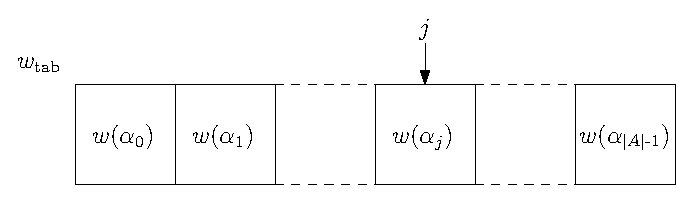
\includegraphics[scale=0.85]{figures/wtab}
\end{figure}
Afin d'itérer sur les actions possibles d'un état
$s_i \in S$, i.e., $A(s_i)$, où $i \in \{0, \dots, |S| - 1 \}$, on crée un tableau $succ$ de
taille $|S|$. Pour tout $i \in \{0, \dots, |S| - 1 \}$, l'entrée $i$ du tableau
contient un tuple, contenant lui-même deux tableaux. Le premier tableau,
$A_i$, est
un tableau contenant les indices des actions de $A(s_i)$, i.e.,
\[j \in A_i \iff \alpha_j \in A(s_i),\] avec $j \in \{0, \dots, |A| - 1\}$ et
$\alpha_j \in A$, la $j^\text{ème}$ action de $A$. Le second tableau est le
tableau des successeurs de $s_i$, $\alpha\text{-}succ_i$.
Il contient un tableau pour chaque action possible de $s_i$.
Soit $k \in \{ 0, \dots, |A(s_i)| - 1 \}$, ce tableau respecte la propriété
suivante :
\[
	A_i[k] = j \iff
	\forall (s_{i'}, pr) \in SuccPr(s_i, \alpha_j), \; (i', pr) \in
	\alpha\text{-}succ_i[k]
\]

\begin{figure}[H]
	\captionsetup{justification=centering}
	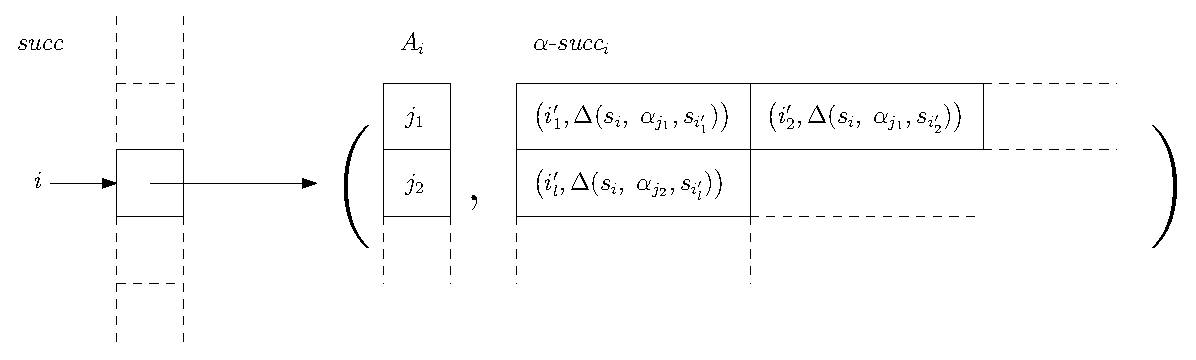
\includegraphics[scale=0.83]{figures/alphasucctab}
\end{figure}

Cette façon de stocker les successeurs de $s_i \in S$ est intéressante, car cela
permet d'obtenir en $\mathcal{O}(1)$ les actions possibles de $s_i$
(en récupérant $A_i$). \par
%Lorsqu'une action $\alpha_j $ est ajoutée dans $Act_i$
%avec l'ensemle des successeurs-$\alpha_j$ de $s_i$ dans le tableau $\alpha$-$succ_i$,
%2 autres tableaux de taille $|S|$ sont mis à jour. Il s'agit des tableaux $pred$ et
%$\alpha$-$pred$ qui représentent respectivement les prédécesseurs de $s_i$
%dans le graphe sous-jacent de $\mathcal{M}$ et les tuples
%$(s, \alpha) \in Pred(s_i)$. En effet, lorsque $j \in \{0, \dots, |A| - 1
%\}$ est ajouté dans $A_i$, dans l'entrée $k$ de ce tableau, et que
%$alpha$-$succ_i[k]$ est initialisé avec les éléments de $SuccPr(s_i, \alpha_j)$,
%ces ceux tableaux sont mis à jour de la façon suivante :
Il reste à définir deux autres tableaux de taille $|S|$ qui vont permettre de
stocker les prédecesseurs de chaque état, pour de cette façon pouvoir accéder
à leurs valeurs en $\mathcal{O}(1)$.
Il s'agit des tableaux $pred$ et
$\alpha$-$pred$ qui représentent respectivement les prédécesseurs de tout $s_i \in S$
dans le graphe sous-jacent de $\mathcal{M}$ et les tuples
$(s, \alpha) \in Pred(s_i)$
, et cela pour tout $i \in \{0, \dots, |S| - 1 \}$
. Soient $k \in \{0, \dots, |A(s_i)| - 1 \}$ et
$j \in \{0, \dots, |A| - 1\}$ tels que $A_i[k] = j$, les deux tableaux respectent
la propriété suivante :
\[
	\forall (i', pr) \in \alpha\text{-}succ_i[k], \; i \in pred[i'] \; \wedge \;
	(i, k) \in \alpha\textit{-}pred[i']
\]
De cette façon, pour tout $i' \in \{0, \dots, |S| - 1 \}$,
\begin{itemize}
	\renewcommand{\labelitemi}{\tiny$\bullet$}
	\item $pred[i']$ est une table de hachage contenant tous les indices des
		prédecesseurs de $s_{i'}$ dans le graphe sous-jacent de $\mathcal{M}$.
	\item $\alpha$-$pred[i']$ est un tableau de tuples contenant tous les indices
		des états et des actions possibles de ces états, qui eux-même sont éléments
		de l'ensemble $Pred(s_{i'})$.
\end{itemize}
L'intérêt d'utiliser une table de hachage pour stocker les éléments de
$pred[i']$ est que, contrairement aux éléments de $\alpha$-$pred[i']$, pour tout $i \in \{0, \dots, |S| - 1 \}$, lorsqu'il existe une action $\alpha \in A(s_i)$ telle qu'un
successeur-$\alpha$ de $s_i$ est
ajouté au tableau $\alpha$-$succ_i$, $i$ peut déjà avoir été ajouté auparavant
dans $pred[i']$ si il existe une autre action $\beta \in A(s_i)$ telle que $\Delta(s_i, \beta, s_{i'}) > 0$, i.e., si $s_{i'}$ est un successeur-$\beta$ de $s_i$. La vérification que cet élément se trouve déjà dans $pred[i']$, afin de ne pas l'y ajouter si il s'y trouve déjà,
se fait donc en moyenne en $\mathcal{O}(1)$.\\

Dans la suite de ce document, lorsque des algorithmes vont traiter de
manipulation de PDMP $\mathcal{M} = (S, A, \Delta, w)$, on va considérer la
représentation de $\mathcal{M}$ par la structure de données décrite ci-dessus, i.e., soient $i \in \{0, \dots, |S| - 1 \}$,
$j \in \{0, \dots, |A| - 1 \}$ et $k \in \{0, \dots, |A(s_i)| - 1 \}$,
\begin{itemize}
	\renewcommand{\labelitemi}{\tiny$\bullet$}
	\item $S := \{0, \dots, |S| - 1 \}$
	\item $A := \{0, \dots, |A| - 1 \}$
	\item $w(\alpha_j) := w_{\text{tab}}[j]$
	\item $Act(s_i) := A_i$
	\item $SuccPr(s_i, \alpha_j) := \alpha$-$succ_i[k]$ où $A_i[k] = j$ (i.e.,
		$\alpha_j \in A(s_i)$)
	\item $pred(s_i) := pred[i]$
	\item $Pred(s_i) := \alpha\text{-}pred[i]$
\end{itemize}


\section{Solveurs}
Dans cette section, nous allons aborder la façon dont les problèmes rencontrés
au chapitre précédent ont été implémentés.
\subsection{Problème d'accessibilité} \label{reach-impl}
Soient $\mathcal{M} = (S, A, \Delta, w)$, un PDMP et $T \subseteq S$, un
sous-ensemble d'états cibles (cf. section \ref{reachability-PDM}).
On souhaite définir une stratégie qui résout le problème d'accessibilité à $T$
pour $\mathcal{M}$.
Pour ce faire, on va construire un vecteur $(x_s)_{s \in S}$
tel que $\forall s \in S$, $x_s = \pr_s^{\max}(\Diamond T)$.
Résoudre le problème d'accessibilité à $T$ pour le PDM $\mathcal{M}$ se déroule
en plusieurs étapes :
\begin{enumerate}
	\item Déterminer les états $s$ qui ne sont pas connexes à $T$ dans
		$G^\mathcal{M}$ pour pouvoir fixer la valeur de $x_s$ à $0$.
	\item Déterminer les états $s$ pour lesquels $\pr^{\max}_s(\Diamond T) = 1$ afin de fixer la valeur de $x_s$ à $1$.
	\item Générer un PL comme décrit au théorème \ref{LP-acc} sans générer
		de contraintes supplémentaires pour les états $s$ dont $x_s$ a déjà été fixé.
	\item Déterminer les actions de $A^{\max}$ et générer un nouveau PDM
		$\mathcal{M}^{\max}$ qui ne considère
		que les actions de cette ensemble pour pouvoir ensuite construire une
		stratégie sans mémoire
		optimale qui résout le problème (cf. preuve du lemme \ref{strat-proof}).
\end{enumerate}

Aborder la construction du vecteur $(x_s)_{s \in S}$ de cette façon permet de
limiter les calculs effectués par le solveur de PL en limitant le nombre de
contraintes générées.

\subsubsection*{Déterminer les états non-connexes à $T$}
Afin de déterminer les états qui ne sont pas connexes à $T$, on va réaliser un
parcours arrière du graphe sous-jacent $G^\mathcal{M}$ depuis le sous-ensemble
d'états cibles $T$ et marquer les états rencontrés lors de ce parcours.
Lorsque le parcours est terminé, les états qui ne sont pas marqués ne sont pas
connexes à $T$.

\begin{algorithm}[H]
\caption{Parcours en largeur arrière}
\hspace*{\algorithmicindent} \textbf{Entrées}:
	\begin{itemize}
		\renewcommand{\labelitemi}{\tiny$\bullet$}
		\item $G=(S, E)$, un graphe.
		\item $T \subseteq S$, un sous-ensemble de sommets.
	\end{itemize}
\hspace*{\algorithmicindent} \textbf{Sortie} :
\begin{itemize}
	\renewcommand{\labelitemi}{\tiny$\bullet$}
	\item $marque$, un tableau de taille
	$|S|$ tel que $\forall s \in S$, $marque[s] = Vrai$ ssi $s$ est connexe à $T$
	dans $G$.
\end{itemize}
\begin{algorithmic}[1]
\STATE $marque \gets $ initialiser un tableau de taille $|S|$ dont tous les
	éléments sont $Faux$
\STATE $\textit{prédécesseurs} \gets $ initialiser file
\FORALL{$t \in T$}
	\STATE $marque[t] \gets Vrai$
	\FORALL{$s' \in pred(t)$}
		\STATE $enfiler(\textit{prédécesseurs},\, s')$
	\ENDFOR
\ENDFOR
\WHILE{$\textit{prédécesseurs}$ non vide}
	\STATE $s \gets \textit{défiler}(\textit{prédécesseurs})$
	\IF{non $marque[s]$}
		\STATE $marque[s] \gets Vrai$
		\FORALL{$s' \in pred(s)$}
			\STATE $enfiler(prececesseurs,\, s')$
		\ENDFOR
	\ENDIF
\ENDWHILE
\RETURN $marque$
\end{algorithmic}
\end{algorithm}

L'algorithme parcourt les sommets du graphe sous-jacent $G^\mathcal{M} = (S, E)$
depuis le sous-ensemble $T$
. En pratique, le parcours des sommets du graphe sous-jacent est réalisé en itérant sur
l'ensemble de prédécesseurs $pred$ défini dans la structure de données du PDM (cf. section \ref{sdd}). Dans le pire des cas, il existe un chemin de $s$ à $T$ pour tout $s \in S$, et
tous les sommets sont visités et marqués à la fin de l'algorithme.
Si les sommets ont déjà été marqués lors de l'exécution, alors ils ne peuvent plus être marqués par
la suite. Chaque sommet n'est donc visité dans le pire des cas qu'une unique fois par l'algorithme.
Lors de l'exécution, pour chaque sommet non-marqué que l'algorithme visite, celui-ci  vérifie si ses
prédecesseurs sont déjà marqués, i.e., l'algorithme vérifie chaque arc entrant du sommet considéré. Dans le pire des cas, l'algorithme a donc vérifié une unique fois tous les arcs du graphe à la fin de l'exécution.
Le temps d'exécution de l'algorithme est donc en $\mathcal{O}(|S| + |E|)$.

\subsubsection*{Déterminer les états $s$ pour lesquels $\pr^{\max}_s (\Diamond T) = 1$}
\textit{L'algorithme suivant provient du livre Principle of
Model checking \cite{DBLP:books/daglib/0020348}}. En pratique, bien que le PL
se résout en temps polynomial, il est nettement plus efficace de prétraiter
les états du PDM afin de déterminer les états $s$ pour lesquels
$\pr^{\max}_s(\Diamond T) = 1$, afin d'ensuite générer les contraintes du PL
pour les états $s$ pour lesquels $x_s$ n'a pas encore été fixé.

\begin{algorithm}[H]
\caption{Trouver les états $s$ tels que $\pr^{\max}_s(\Diamond T) = 1$}
\hspace*{\algorithmicindent} \textbf{Entrées}:
	\begin{itemize}
		\renewcommand{\labelitemi}{\tiny$\bullet$}
		\item $\mathcal{M} = (S, A, \Delta)$, un PDM fini.
		\item $T \subseteq S$, un sous-ensemble d'états cibles.
	\end{itemize}
\hspace*{\algorithmicindent} \textbf{Sortie} :
\begin{itemize}
	\renewcommand{\labelitemi}{\tiny$\bullet$}
	\item Les états $s$ du PDM tels que
		$\pr_{s}^{\max} (\Diamond T)= 1$.
\end{itemize}
\begin{algorithmic}[1]
\STATE $U \gets \{ s \in S \; | \; s \text{ est non-connexe à } T \text{ dans } G^\mathcal{M}\}$
\WHILE{$U \neq \varnothing$}
	\STATE $R \gets U$
	\WHILE{$R \neq \varnothing$}
		\STATE Soit $u \in R$
		\STATE $R \gets R \setminus \{u \}$
		\FORALL{$(s, \alpha) \in Pred(u)$ tel que $s \not\in U \cup T$}
			\STATE supprimer $\alpha$ de $A(s)$
			\IF{$A(s) = \varnothing$}
				\STATE $R \gets R \cup \{s\}$
				\STATE $U \gets U \cup \{s\}$
			\ENDIF
		\ENDFOR
		\COMMENT{tous les arcs entrants de $u$ ont maintenant été supprimés}
		\STATE supprimer $u$ et ses arcs sortants dans $\mathcal{M}$
	\ENDWHILE
	\COMMENT{{\footnotesize il faut maintenant recalculer les états qui ne peuvent pas atteindre $T$ dans le PDM modifié}}
	\STATE $U \gets \{ s \in S \setminus U \; | \; s \text{ n'est pas connexe à } T \text{ dans } G^\mathcal{M} \}$
\ENDWHILE
\RETURN les états restants du MDP
\end{algorithmic}
\end{algorithm}

L'algorithme abordé ci-dessus est exact et est polynomial en $|\mathcal{M}|$.
Cependant, le pseudo-code de cet algorithme est de très haut niveau. On va maintenant l'adapter à
la structure de données du PDM que l'on a défini plus tôt dans ce document.

\begin{algorithm}[H]
%\caption{Trouver les états $s$ tels que $\pr^{\max}_s(\Diamond T) = 1$}
\caption{PrMax1}
\hspace*{\algorithmicindent} \textbf{Entrées}:
	\begin{itemize}
		\renewcommand{\labelitemi}{\tiny$\bullet$}
		\item $\mathcal{M} = (S, A, \Delta)$, un PDM fini.
		\item $T \subseteq S$, un sous-ensemble d'états cibles.
	\end{itemize}
\hspace*{\algorithmicindent} \textbf{Sortie} :
\begin{itemize}
	\renewcommand{\labelitemi}{\tiny$\bullet$}
	\item $S^{\max}_{=1}$, une liste contenant les sommets du PDM tel que $\forall s \in S^{\max}_{=1},
		\; \pr_{s}^{\max} (\Diamond T)= 1$.
\end{itemize}
\begin{algorithmic}[1]
\STATE $\textit{connecté} \gets \textit{ParcoursLargeurArrière}(G^\mathcal{M},\, T)$
\STATE $\textit{supprimé} \gets$ initialiser tableau de taille $|S|$ dont
	les éléments sont $Faux$
\STATE $\textit{actionSupprimée} \gets$ initialiser tableau de taille
	$|S|$
\FORALL{$s \in S$}
	\STATE $\textit{actionSupprimée}[s] \gets$ {\small initialiser tableau de taille $|A(s)|$
		dont les éléments sont $Faux$}
\ENDFOR
\STATE $\textit{nombreActionsSupprimées} \gets$ {\small initialiser tableau de taille $|S|$ dont les éléments sont $0$}
\WHILE{$compter(\lambda s: \text{non }\textit{connecté}[s] \text{ et non } \textit{supprimé}[s], \, S) > 0$}
	\STATE $R \gets $ initialiser file
	\FORALL{$s \in S$}
		\IF{non $\textit{connecté}[s]$ et non $\textit{supprimé}[s]$}
			\STATE $enfiler(R, \, s)$
		\ENDIF
	\ENDFOR
	\WHILE{$R$ non vide}
		\STATE $u \gets \textit{défiler}(R)$
		\FORALL{$(s, \alpha) \in Pred(u)$}
			\IF{$\textit{connecté}[s]$ et non $\textit{actionSupprimée}[s][\alpha]$ et
				 $s \not\in T$}
				\STATE $\textit{actionSupprimée}[s][\alpha] \gets Vrai$
				\STATE $\textit{nombreActionsSupprimées}[s] \gets \textit{nombreActionsSupprimées}[s] + 1$
				\IF{$\textit{nombreActionsSupprimées}[s] = |A(s)|$}
					\STATE $enfiler(R, \, s)$
					\STATE $\textit{connecté}[s] \gets Faux$
				\ENDIF
			\ENDIF
		\ENDFOR
		\STATE $\textit{supprimé}[u] \gets Vrai$
	\ENDWHILE
	\STATE $G = (S, E) \gets $initialiser Graphe avec $E$ vide
	\FORALL{$s \in S$}
		\IF{non \textit{supprimé}[s]}
			\FORALL{$\alpha \in A(s)$}
				\IF{non $\textit{actionSupprimée}[\alpha]$}
					\FORALL{$(s', pr) \in SuccPr(s, \alpha)$}
						\IF{non $\textit{supprimé}[s']$}
							\STATE $ajouterArc\big(E,\, (s, s') \big)$
						\ENDIF
					\ENDFOR
				\ENDIF
			\ENDFOR
		\ENDIF
	\ENDFOR
	\STATE $\textit{connecté} \gets \textit{ParcoursLargeurArrière}(G, \, T)$
\ENDWHILE
\STATE $S^{\max}_{=1} \gets$ initialiser liste
\FORALL{$s \in S$}
	\IF{non \textit{supprimée}$[s]$}
		\STATE $ajouter(S^{\max}_{=1}, \, s)$
	\ENDIF
\ENDFOR
\RETURN $S^{\max}_{=1}$
\end{algorithmic}
\end{algorithm}
	%\STATE $\mathcal{M}' \gets (S', A', \Delta)$ tel que, soit $s \in S$
	%	\begin{itemize}
	%		\renewcommand{\labelitemi}{\tiny$\bullet$}
	%		\item $s \in S'$ ssi non $\textit{supprimé}[s]$
	%		\item $\alpha \in A'(s)$ ssi non $\textit{actionSupprimée}[s][\alpha]$
	%	\end{itemize}
\newpage
\textit{Notation:} $\lambda x: v$ est une notation qui se base sur le
lambda-calcul (cf. ligne 7). En effet, cela représente une fonction qui
associe $x$ à $v$, où $v$ contient en général des occurences de $x$ (en
lambda-calcul : $\lambda x.v$). \\

\textit{Commentaires :}
\begin{itemize}
	\renewcommand{\labelitemi}{\tiny$\bullet$}
	\item Tous les tableaux de booléens peuvent être remplacés par des tables de
		hachage. En effet,
		\begin{itemize}
			\item Définir la valeur d'un état à $Vrai$ dans le tableau est équivalent
				à ajouter un état dans la table de hachage.
			\item Vérifier que la valeur d'un état est $Vrai$ dans le tableau équivaut
				à vérifier qu'un état se trouve dans la table de hachage.
		\end{itemize}
		Les différences résident en la complexité en mémoire et en temps des 2 structures de données.
		\begin{itemize}
			\item L'espace occupé par les tableaux en mémoire est fixe, tandis que celui occupé par les tables de hachage est alloué dynamiquement en fonction du nombre d'éléments présents à l'intérieur.
			Les tables de hachage
				occupent dans la plupart des cas moins d'espace en mémoire que les tableaux, surtout dans le cas où la plupart des états
				sont connexes à $T$ et lorsque peu d'actions mènent le système vers un
				état non-connexe à $T$. Cependant, par le fait que la mémoire est allouée dynamiquement, lorsqu'un nombre conséquent d'états sont liés
				à des états non-connexes à $T$, la mémoire allouée aux tables de hachage se rapproche fortement de celle des tableaux (et peut même dans le pire des cas la dépasser). Ce phénomène n'est pas rare dans le cas de
				la résolution du problème des plus courts chemins stochastiques de taille limitée.
			\item La complexité en temps de la vérification qu'un état a pour valeur
				$Vrai$ dans un tableau est toujours en $\mathcal{O}(1)$, tandis que
				la vérification que l'état se trouve dans la table de hachage est en
				moyenne en $\mathcal{O}(1)$, mais peut aller jusque $\mathcal{O}(|S|)$,
				voir $\mathcal{O}(|S| \times |A|)$ dans le pire des cas pour certaines
				tables en Python (cf. TimeComplexity dans la documentation officielle des \textit{set} de Python).
		\end{itemize}
		La performance en terme de complexité (en mémoire et en temps) de ces deux
		approches dépendent donc entièrement du PDM traité. On fait ici le choix
		d'assurer une complexité en temps optimale au détriment de la complexité
		en mémoire.
		\item On suppose que la fonction $compter$ (cf. ligne 7) compte les éléments d'une
			structure de données qui respectent la propriété entrée en paramètre de la fonction.
			Dans notre cas, la fonction retourne le nombre d'états qui ne sont pas
			connectés à $T$ et qui n'ont pas encore été supprimés.
		\item On suppose que l'action d'ajouter un arc $(s, s')$ au graphe (cf.
			ligne 29) met à jour la table de hachage représentant les prédécesseurs de $s'$ dans ce graphe, i.e., $pred(s') \gets \{s\} \cup pred(s')$.
	\end{itemize}

\subsubsection*{Générer le PL}
Lors des $2$ étapes précédentes, on a fixé la valeur de $x_s$ à 0 pour les états
$s$ non-connexes à $T$ dans le graphe sous jacent $G^\mathcal{M}$ et on a fixé
les valeurs de $x_s$ à 1 pour les états $s$ tels que $\pr^{\max}_s(\Diamond T) = 1$. Il reste à générer les contraintes du PL pour le reste des états (cf. théorème \ref{LP-acc}).
Afin de générer un PL, on utilise le package \verb|PuLP| de
\verb|python 3|. Ce package permet de modéliser des programmes linéaires de
façon très intuitive en python (cf. figure \ref{reach-pulp}) et de les résoudre à partir de solveurs
externes au choix (\verb|GLPK|, \verb|CPLEX|, \verb|COIN CLP/CBC|, \verb|GUROBI|, etc.).
Par défaut, le solveur utilisé sera \verb|GLPK|, mais le programme permet
d'indiquer quel solveur utiliser.
\begin{figure}[H]
	\centering
	\scriptsize
	\inputminted{python}{PLexample.py}
	\cprotect\caption{Génération des contraintes du PL avec \verb|PuLP|.}
	\label{reach-pulp}
\end{figure}

\subsubsection*{Construire la stratégie}
Une fois que le vecteur $(v_s)_{s \in S}$ représentant la solution du PL
est calculé, on peut construire la stratégie qui va résoudre le problème
d'accessibilité du PDM $\mathcal{M}$. L'algorithme suivant se base sur la preuve du lemme \ref{strat-proof} dans laquelle on construit la stratégie
optimale du problème d'accessibilité.

\begin{algorithm}[H]
\caption{Construire la stratégie optimale pour le problème d'accessibilité}
\hspace*{\algorithmicindent} \textbf{Entrées}:
	\begin{itemize}
		\renewcommand{\labelitemi}{\tiny$\bullet$}
		\item $\mathcal{M} = (S, A, \Delta)$, un PDM.
		\item $v$, un tableau pour lequel $v[s] = \pr^{\max}_s(\Diamond T) \; \forall s \in S$ .
	\end{itemize}
\hspace*{\algorithmicindent} \textbf{Sortie} :
\begin{itemize}
	\renewcommand{\labelitemi}{\tiny$\bullet$}
	\item la stratégie optimale qui résout le problème d'accessibilité de $\mathcal{M}$.
\end{itemize}
\begin{algorithmic}[1]
\STATE $A^{\max} \gets$ initialiser ensemble d'actions de PDM
\FORALL{$s \in S$}
	\FORALL{$\alpha \in A(s)$}
		\STATE $pr \gets \sum_{(s', \,pr) \in SuccPr(s, \alpha)} pr \cdot v[s']$
		\IF{$pr = v[s]$}
			\STATE $ajouter(A^{\max}(s), \, \alpha)$
		\ENDIF
	\ENDFOR
\ENDFOR
\STATE $\mathcal{M}^{\max} = (S,\, A^{\max}) \gets $ initialiser PDM
\STATE $\textit{étapes} \gets PlusCourtChemin(G^{\mathcal{M}^{\max}},\, T)$
\STATE $A^* \gets$ initialiser tableau de taille $|S|$
\FORALL{$s \in S$}
	\STATE $A^*[s] \gets \alpha \in A^{\max}(s)$
	\COMMENT{initialiser $A^*[s]$ avec une action arbitraire}
	\FORALL{$\alpha \in A^{\max}(s)$}
		\FORALL{$(s', pr) \in SuccPr(s, \alpha)$}
			\IF{\textit{étapes}$[s] - 1 = \textit{étapes}[s']$}
				\STATE $A^*[s] \gets \alpha$
			\ENDIF
		\ENDFOR
	\ENDFOR
\ENDFOR
\RETURN $\lambda s: \; A^*[s]$
\end{algorithmic}
\end{algorithm}

Il reste maintenant à définir l'algorithme des plus courts chemins (en terme d'étapes) dans le
graphe sous-jacent pour tout sommet $s$ vers le sous-ensemble des sommets
$T$. Pour ce faire, on adapte l'algorithme de parcours en largeur arrière pour
numéroter les sommets en fonction de l'itération, i.e., l'étape à laquelle les sommets ont été visités.

\begin{algorithm}[H]
\caption{Parcours en largeur arrière : plus court chemin}
\hspace*{\algorithmicindent} \textbf{Entrées}:
	\begin{itemize}
		\renewcommand{\labelitemi}{\tiny$\bullet$}
		\item $G=(S, E)$, un graphe.
		\item $T \subseteq S$, un sous-ensemble de sommets.
	\end{itemize}
\hspace*{\algorithmicindent} \textbf{Sortie} :
\begin{itemize}
	\renewcommand{\labelitemi}{\tiny$\bullet$}
	\item $\textit{étapes}$, un tableau de taille $|S|$ tel que $\forall s \in
	S$, \textit{étapes}$[s]$ correspond au plus court chemin en terme d'étapes,
	i.e., du nombre d'arcs minimum parcourus pour atteindre le sous-ensemble
	$T$.
\end{itemize}
\begin{algorithmic}[1]
\STATE $\textit{étapes} \gets$ initialiser un tableau de taille $|S|$ dont
tous les éléments sont $\infty$
\STATE $\textit{étapeSuivante} \gets $ initialiser file
\STATE $i \gets 0$
\FORALL{$t \in T$}
	\STATE $\textit{étapes}[t] \gets i$
	\FORALL{$s' \in pred(t)$}
		\STATE $enfiler(\textit{étapeSuivante},\, s')$
	\ENDFOR
\ENDFOR
\WHILE{$\textit{étapeSuivante}$ non vide}
	\STATE $i \gets i + 1$
	\STATE \textit{prédécesseurs}$\gets \textit{étapeSuivante}$
	\STATE \textit{étapeSuivante}$\gets$ initialiser liste vide
	\WHILE{\textit{prédécesseurs} non vide}
		\STATE $s \gets \textit{défiler}(\textit{prédécesseurs})$
		\IF{$\textit{étapes}[s] = \infty$}
			\STATE $\textit{étapes}[s] = i$
			\FORALL{$s' \in pred(s)$}
				\STATE $enfiler(\textit{étapeSuivante},\, s')$
			\ENDFOR
		\ENDIF
	\ENDWHILE
\ENDWHILE
\RETURN$\textit{étapes}$
\end{algorithmic}
\end{algorithm}

La complexité en temps de cet algorithme est identique au parcours en largeur
classique ; dans le pire des cas, les états sont visités une unique fois et
les arcs sont également visités une unique fois. La complexité en temps de
l'algorithme est donc en $\mathcal{O}(|S| + |E|)$. On va prouver que la boucle
externe de l'algorithme (cf. ligne 8) possède l'invariant suivant:
$\forall s \in S, \; \textit{étapes}[s]$ est la taille du chemin le plus court de $s$ à
$T$ dans $G$ avec un chemin de taille inférieure ou égale à $i$, où $i$ est
le nombre d'itérations effectuées par la boucle externe. \\
	\textbf{Cas de base} : $i = 0$, i.e., lorsque l'algorithme entre dans
		la boucle externe. L'algorithme initialise \textit{étapes}$[t]$ $\forall t \in T$ à $0$ (cf. lignes 4 et 5). On a bien que $\textit{étapes}[t]$
		correspond à la taille du chemin le plus court de $t$ à $T$. \\
	\textbf{Cas général} : Soit $i \in \mathbb{N}$. On suppose qu'on a, à la fin
		de la $i^{\text{ème}}$ itération de la boucle externe, que
		$\textit{étapes}[s]$ est la taille du chemin le plus court de $s$ à $T$ avec un
		chemin de taille inférieure ou égale à $i$. Pendant l'étape $i$, tous les
		arcs entrants $(s, s')$ des sommets $s'$ tels que $\textit{étapes}[s'] =
		i$ sont visités (cf. ligne 17). Les prédécesseurs de $s'$ sont de cette
		manière ajoutés à la file \textit{étapeSuivante}. Il s'agit des sommets
		qui vont être traités à l'étape courante $i+1$ (cf. lignes 10 et 12).
		Pour chaque sommet $s \in S$ traité à l'étape courante,
		\begin{itemize}
			\item Si \textit{étapes}$[s] < i + 1$, alors on a que le sommet a déjà
				été visité lors des itérations précédentes de la boucle externe et on
				a donc par hypothèse que \textit{étapes}$[s]$ est la taille du chemin le plus
				court depuis $s$ vers $T$.
			\item Si \textit{étapes}$[s] > i$, alors c'est que $\textit{étapes}[s]$
				n'a pas encore été visité par l'algorithme et que $\textit{étapes}[s] = \infty$.
				Vu que le sommet n'a pas encore été visité, l'algorithme le marque en
				fixant la valeur de $\textit{étapes}[s]$ à $i + 1$ (cf. lignes 14
				et 15). En effet, vu que $\textit{étapes}[s]$ n'avait pas été traité
				lors des itérations précédentes, cela signifie qu'il n'existe pas de
				chemin de longueur strictement inférieure à $i+1$ de $s$ à $T$ dans le graphe
				(sinon, par hypothèse, le sommet aurait été marqué lors des itérations précédentes).
				De plus, vu qu'il existe un arc $(s, s') \in E$ tel que
				$\textit{étapes}[s'] = i$ et tel que $\textit{étapes}[s']$ est le plus
				court chemin de $s'$ à $T$, on a bien qu'il existe un chemin de $s$ à
				$T$, que ce chemin est de longueur $i + 1$ et qu'il est le
				plus court pour atteindre $T$ depuis $s$.
		\end{itemize}
Par induction sur $i$, on prouve l'invariant. Comme l'algorithme visite
dans le pire des cas une unique fois tous les sommets et tous les arcs de $G$,
on a forcément que l'algorithme s'arrête car la file \textit{étapeSuivante}
finit par être vide (cf. ligne 8). Cela mène au fait que, pour tout sommet $s \in S$,
$\textit{étapes}[s]$ est la longueur du chemin le plus court de $s$ à $T$.

\subsection{Problème de l'espérance du plus court chemin stochastique}
Soient $\mathcal{M} = (S, A, \Delta, w)$, un PDMP, $T \subseteq S$, un
sous-ensemble d'états cibles et $l \in \mathbb{N}$, un seuil de longueur.
On souhaite définir une stratégie qui résout le problème de l'espérance du plus
court chemin stochastique pour le PDMP $\mathcal{M}$ jusqu'au sous-ensemble
d'états cibles $T$ sous le seuil de longueur $l$ (cf. sous-section \ref{sspe}).
Tout d'abord, on génère le PL du théorème \ref{esp-PDMP} à l'aide du package
\verb|PuLP| de Python. On utilise ensuite un solveur supporté par \verb|PuLP| (e.g., \verb|GLPK|)
afin de résoudre le PL. La solution de ce PL est un tableau $v$ de taille
$|S|$ tel que $v[s] = \min_{\sigma} \mathbb{E}_s^\sigma(TS^T)$ pour
tout $s \in S$. On construit la stratégie $\sigma$ comme décrit dans
le théorème \ref{esp-PDMP}. Soit $s \in S$. Dès lors, $v[s] =
\mathbb{E}_s^\sigma(TS^T)$. Si $v[s] \leq l$, alors la stratégie
$\sigma$ résout le problème d'espérance du plus court chemin stochastique
sous le seuil de longueur $l$ de l'état $s$ aux états cibles de $T$ dans
$\mathcal{M}$.

\begin{algorithm}[H]
\caption{Résoudre le problème de l'espérance du plus court chemin stochastique}
\hspace*{\algorithmicindent} \textbf{Entrées}:
	\begin{itemize}
		\renewcommand{\labelitemi}{\tiny$\bullet$}
		\item $\mathcal{M} = (S, A, \Delta, w)$, un PDMP.
		\item $s \in S$, un état de $\mathcal{M}$.
		\item $T \subseteq S$, un sous-ensemble d'états de $\mathcal{M}$.
		\item $l \in \mathbb{N}$, un seuil de longueur.
	\end{itemize}
\hspace*{\algorithmicindent} \textbf{Sortie} :
\begin{itemize}
	\renewcommand{\labelitemi}{\tiny$\bullet$}
	\item $Vrai$ si il existe une stratégie $\sigma$ pour laquelle $\mathbb{E}^{\sigma}_s (TS^T) \leq l$, $Faux$ sinon.
\end{itemize}
\begin{algorithmic}[1]
\STATE $(v, \sigma) \gets \textit{ConstruireStratégieOptimale}(\mathcal{M}, \, T)$
\IF{$v[s] \leq l$}
	\RETURN $Vrai$
\ELSE
	\RETURN $Faux$
\ENDIF
\end{algorithmic}
\end{algorithm}

\begin{algorithm}[H]
\caption{Construire la stratégie optimale pour le problème de l'espérance du plus court chemin stochastique}
\hspace*{\algorithmicindent} \textbf{Entrées}:
	\begin{itemize}
		\renewcommand{\labelitemi}{\tiny$\bullet$}
		\item $\mathcal{M} = (S, A, \Delta, w)$, un PDMP.
		\item $T \subseteq S$, un sous-ensemble d'états cibles.
	\end{itemize}
\hspace*{\algorithmicindent} \textbf{Sortie} :
\begin{itemize}
	\renewcommand{\labelitemi}{\tiny$\bullet$}
	\item $v$, un tableau de taille $|S|$ tel que $ \forall s \in S,\, v[s] = \min_{\sigma} \mathbb{E}_s^\sigma(TS^T)$.
	\item $\sigma$, la stratégie optimale telle que $\forall s \in S, \, v[s] = \mathbb{E}_s^\sigma(TS^T)$.
\end{itemize}
\begin{algorithmic}[1]
\STATE $x \gets$ initialiser un tableau de taille $|S|$
\STATE $pl \gets$ initialiser PL
\FORALL{$s \in S$}
	\STATE $initialiserVariable(pl,\, x[s])$
\ENDFOR
\STATE $p_1 \gets prMax1(\mathcal{M}, \, T)$
\STATE $objectif(pl,\, \max, \, \sum_{s \in p1} x[s])$
\FORALL{$s \in S$}
	\IF{$s \in T$}
		\STATE $x[s] \gets 0$
	\ELSIF{$s \not \in p_1$}
		\STATE $x[s] \gets \infty$
	\ELSE
		\FORALL{$\alpha \in A(s)$}
			\STATE $ajouterContrainte\big(pl,\, x[s] \leq w(\alpha) +  \sum_{(succ, pr) \in SuccPr(s, \alpha)} pr \cdot x[succ] \big)$
		\ENDFOR
	\ENDIF
\ENDFOR
\STATE $v \gets \textit{résoudre}(pl)$
\RETURN $\big(v, \; \lambda s: \arg \min_{\alpha \in A(s)} \big( w(\alpha) + \sum_{(succ, pr) \in SuccPr(s, \alpha)} pr \cdot v[succ] \big)\big)$
\end{algorithmic}
\end{algorithm}

\subsection{Problème des plus courts chemins stochastiques de taille limitée}
Soient $\mathcal{M} = (S, A, \Delta, w)$, un PDMP, $l \in \mathbb{N}$, la
longueur maximale des chemins que l'on va traiter, $s \in S$, un état de
$\mathcal{M}$ et $b \in [0, 1] \cap \mathbb{Q}$, un seuil de probabilité.
On souhaite définir une stratégie qui résout le problème des plus courts
chemins stochastiques limités par le seuil $l$ depuis l'état $s$ jusqu'au sous-ensemble
d'états cibles $T$ au dessus du seuil de probabilité $b$ (cf. sous-section \ref{sspp}).
Le problème se résout en 3 étapes.
\begin{enumerate}
	\item \textit{"Déplier"} le PDMP $\mathcal{M}$ depuis l'état $s$ afin de créer un
		nouveau PDM $\mathcal{M}' = (S', A', \Delta')$.
	\item %Calculer la stratégie $\sigma$ qui résout le problème
		%d'accessibilité pour $\mathcal{M}'$. Il est également nécessaire de
		Construire un vecteur $(v_{s'})_{s' \in S'}$ tel que pour tout $s' \in S'$, $v_{s'} =
		\pr^{\max}_{s'} (\Diamond T')$ (cf. sous-section \ref{reach-impl}).
	\item Si $v_{(s, 0)} \geq b$, alors la stratégie $\sigma$ optimale
		qui résout le problème d'accessibilité de $\mathcal{M}'$ résout le
		problème des plus courts chemins stochastiques de taille limitée par le seuil $l$ depuis l'état $s$ vers le sous-ensemble d'états cibles $T$.
\end{enumerate}

On veut construire le PDM $\mathcal{M}' = (S', A', \Delta')$ en dépliant
le PDMP $\mathcal{M}$ afin de résoudre le problème d'accessibilité
de $(s, 0)$ à $T' = \{ (t, v) \in S' \; | \; t \in T \wedge v \leq l \}$.
Afin d'assurer une complexité en temps et en mémoire optimale, certaines optimisations peuvent être réalisées lors de la construction de $\mathcal{M}'$ par rapport à sa définition dans la sous-section \ref{sspp}.
\begin{itemize}
	\renewcommand{\labelitemi}{\tiny$\bullet$}
	\item
Premièrement, pour tout état $t' \in T'$, et pour chaque action possible
$\alpha \in A(t')$, il n'est pas nécessaire de considérer les
successeurs-$\alpha$ de $t'$. En effet, par le théorème \ref{LP-acc}, on aura forcément que $x[t'] = \pr^{\max}_{t'}(\Diamond T) = 1$.
%On introduit donc une nouvelle action $\alpha_{\text{loop}}$ telle que $\forall t' \in T'$, $A(t') = \{\alpha_{\text{loop}} \}$ et $\Delta'(t', \alpha_\text{loop}, t') = 1$.
	\item
Ensuite, il n'est pas nécessaire de considérer les états $(s, v)$ de $\mathcal{M}'$ tels que $v = \bot$. En effet, par définition de $T'$, tous ces états sont non-connexes à $T'$ et donc, pour tout $s' \in \{ (s, v) \in S' \; | \; v = \bot \} \subseteq S'$, on aura forcément que $x[s'] = \pr^{\max}_{(s, \bot)} (\Diamond T') = 0$ par le théorème \ref{LP-acc}.
	\item
Finalement, comme on veut résoudre le problème de $(s, 0)$ à $T'$, il n'est pas
nécessaire de construire le PDM déplié complet.
Par le fait que pour tout état $(s, v) \in S'$, $v$ représente la longueur du
chemin courant dans $\mathcal{M}'$, vu que pour tout $\alpha \in A\big((s, v)\big)$,
$w(a) > 0$, on a pour tout successeur-$\alpha$ $(s', v')$ de $(s, v)$ que $v' > v$.
Si on ne prend pas
en compte les états de $S'_\bot = \{ (s, v) \in S' \; | \; v = \bot \}$,
le graphe
sous-jacent $G^{\mathcal{M}'}=(S' \setminus S'_\bot, E)$ prend la forme d'un \textit{DAG} (i.e., graphe
orienté acyclique). La particularité des DAG est qu'il n'existe
pas de circuit dans de tels graphes.
Un circuit d'un graphe orienté $G = (S, E)$ est un chemin fini dont le premier et
dernier sommet sont identiques, i.e., une séquence de sommets $\pi = s_0 \dots s_n \in S^+$ où pour tout $i \in \{0, \dots, n\}$, $(s_i, s_{i+1}) \in E$ et $s_0 = s_n$.
En effet, dans $\mathcal{M}'$, soit $s' \in S' \setminus S'_\bot$, il n'existe pas de chemin fini $\pi = s_0 \alpha_1 s_1 \dots \alpha_n s_n \in Paths_{fin}(s')$
tel que $s_0 = s_n$.
Il est donc uniquement nécessaire de considérer
les états accessibles depuis l'état $(s, 0)$ dans $\mathcal{M}'$.
\end{itemize}

\begin{algorithm}[H]
\caption{Construire $\mathcal{M}'$}
\hspace*{\algorithmicindent} \textbf{Entrées}:
	\begin{itemize}
		\renewcommand{\labelitemi}{\tiny$\bullet$}
		\item $\mathcal{M} = (S, A, \Delta, w)$, un PDMP.
		\item $T \subseteq S$, le sous-ensemble d'états cibles dans $\mathcal{M}$.
		\item $s \in S$, l'état à partir duquel $\mathcal{M}$ va être déplié.
		\item $l \in \mathbb{N}$, le seuil de longueur des chemins de
			$\mathcal{M}$.
	\end{itemize}
\hspace*{\algorithmicindent} \textbf{Sorties} :
	\begin{itemize}
	\renewcommand{\labelitemi}{\tiny$\bullet$}
	\item $\mathcal{M}'$, le PDM déplié depuis l'état $(s, 0)$ de $\mathcal{M}$.
	\item $T' \subseteq S'$, le sous-ensemble d'états cibles dans
		$\mathcal{M}'$
	\end{itemize}
\begin{algorithmic}[1]
\STATE $\mathcal{M}' = (S', A', \Delta') \gets$ initialiser PDM avec $S'$ et $A'$ vides \\
\COMMENT{on remplace l'ensemble $S_\bot$ par un unique état $s_\bot$}
\STATE $ajouter\textit{\'E}tat(S', \, s_\bot)$\\
\COMMENT{on ajoute l'action $\alpha_{loop}$ afin de faire en sorte que $\forall t' \in T', \;
	\Delta(t',\, \alpha_{loop},\, t') = \Delta(s_\bot,\, \alpha_{loop},\, s_\bot) = 1$}
\STATE $ajouterAction(A', \, \alpha_{loop})$
\STATE $ajouterAction(A'(s_\bot), \, \alpha_{loop})$
\STATE $ajouterSuccesseur\big(\mathcal{M}', \, s_\bot, \, \alpha_{loop}, \,
	(s_\bot, 1)\big)$
\STATE $T' \gets$ initialiser sous-ensemble d'états de $\mathcal{M}'$\\
\COMMENT{on associe tout état $s \in S$ de
		$\mathcal{M}$ et la valeur de la longueur de son chemin courant $v \in \mathbb{N}$ à
		un état de $\mathcal{M'}$ à l'aide d'une matrice $V$, i.e., $V[s][v] = (s, v) \in S'$.}
\STATE $V \gets$ initialiser matrice de taille $|S| \times (l + 1)$ dont les éléments sont $-1$
\STATE $\textit{déplier}(s,\, 0)$
\RETURN $(\mathcal{M}', \, T')$
\end{algorithmic}
\end{algorithm}

\textit{Commentaires:}
\begin{itemize}
\renewcommand{\labelitemi}{\tiny$\bullet$}
	\item On suppose que la fonction $ajouterAction$ (ligne 4) met à jour le
		tableau qui représente $A(s_\bot)$ dans $\mathcal{M}'$.
	\item On suppose que la fonction $ajouterSuccesseur$ (ligne 5) met à jour les tableaux
		qui représentent les ensembles $SuccPr$, $Pred$ et la table de hachage qui représente l'ensemble $pred$ dans $\mathcal{M}'$.
		\textit{Note : }ici, $(s_\bot, 1) \in SuccPr(s_\bot, \alpha_{loop})$.
	\item La matrice $V$ peut être remplacée par un tableau de hash map tel que
		$\forall s \in S, \; V[s]$ contient une hash map qui possède comme clés les
		longueurs possibles des chemins courants lorsqu'on se situe dans l'état
		$s$ dans $\mathcal{M}$. En d'autres termes, soit $s \in S$, un état de $\mathcal{M}$ et $v \in \mathbb{N}$, une clé de la hash map $V[s]$, alors
		$V[s][v] = (s, v)$ où $(s, v) \in S'$ est un état de $\mathcal{M}'$.
		La différence réside en la complexité en temps et en
		mémoire des deux approches.
		En effet, $V[s][v]$ se récupère en $\mathcal{O}(1)$ dans la matrice et en
		moyenne en $\mathcal{O}(1)$ dans le tableau de hash map. Cependant, supposons que $\forall \alpha \in A$,
		$w(\alpha)$ est très grand. Dans ce cas, beaucoup de cases sont
		inutilisées dans la matrice car elles ne seront jamais remplies lors du
		dépliage de $\mathcal{M}$. La matrice est particulièrement efficace quand
		les valeurs des poids des actions sont petites car très peu de cases de la matrice sont "gaspillées" et celle-ci permet d'assurer de récupérer les états de $\mathcal{M}'$ en $\mathcal{O}(1)$.
\end{itemize}

\begin{algorithm}[H]
\caption{Déplier}
\hspace*{\algorithmicindent} \textbf{Entrées}:
	\begin{itemize}
		\renewcommand{\labelitemi}{\tiny$\bullet$}
		\item $s \in S$, l'état à partir duquel $\mathcal{M}$ va être déplié.
		\item $v \in \mathbb{N}$, la longueur du chemin courant.
	\end{itemize}
\hspace*{\algorithmicindent} \textbf{Effet de bord} :
	\begin{itemize}
	\renewcommand{\labelitemi}{\tiny$\bullet$}
	\item
	Met à jour et construit le PDM déplié $\mathcal{M}'$, le sous-ensemble d'états cible
	$T'$ et la matrice $V$.
	\end{itemize}
\begin{algorithmic}[1]
\STATE $s' \gets V[s][v]$
\IF{$s' = -1$}
	\STATE $V[s][v] \gets |S'|$
	\STATE $ajouter\textit{\'E}tat(S', \, s')$
	\IF{$s \in T$}
		\STATE $ajouter\textit{\'E}tat(T', \, s')$
		\STATE $ajouterAction(A'(s'), \; \alpha_{loop})$
		\STATE $ajouterSuccesseur(\mathcal{M}', \, s', \alpha_{loop}, (s',1))$
	\ELSE
		\FORALL{$\alpha \in A(s)$}
			\IF{$v + w(\alpha) > l$}
				\STATE $ajouterSuccesseur(\mathcal{M}', \, s', \,  \alpha, \,  (s_\bot, 1))$
			\ELSE
				\FORALL{$(succ, \, pr) \in SuccPr(s, \alpha)$}
					\STATE $v' \gets v + w(\alpha)$
					\STATE $\textit{déplier}(succ, \, v')$
					\STATE $ajouterAction(A'(s'), \, \alpha)$
					\STATE $succ' \gets V[succ][v']$
					\STATE $ajouterSuccesseur(\mathcal{M}', \, s', \, \alpha, \, (succ',pr))$
				\ENDFOR
			\ENDIF
		\ENDFOR
	\ENDIF
\ENDIF
\end{algorithmic}
\end{algorithm}
La complexité en temps du dépliage est intuitive grâce à la matrice $V$. Pour rappel, la matrice $V$ est de taille $|S| \, (l + 1)$ et chaque case remplie correspond à un sommet de $\mathcal{M}'$. \`A chaque appel récursif, on remplit une case de la matrice uniquement
si celle-ci n'a pas encore été remplie. Le pire des cas correspond donc à celui
où toutes les cases de la matrice sont remplies (i.e., celui où le graphe sous-jacent du PDMP est
complet et où toutes les actions $\alpha$ ont un poids de $w(\alpha) = 1$). \`A chaque fois qu'une case est remplie, l'algorithme itère sur les actions
$\alpha$ de chaque état, et ensuite sur ses successeurs-$\alpha$.
On suppose qu'ajouter un état, ajouter une action et ajouter un successeur se
fait en $\mathcal{O}(1)$. De ce fait, traiter une case de $V$ se fait en $\mathcal{O}(|A| \, |S|)$ (le pire des cas est celui où $\forall s \in S, \; |A(s)| = |A|$, i.e., toutes les actions sont possibles pour chaque $s$ et
celui où $\forall \alpha \in A(s), \; |Succ(s, \, \alpha)| = |S|$). De ce fait,
on a que le dépliage du PDMP se fait en $\mathcal{O}(|V| \, |S| \, |A|) = \mathcal{O}(l \, |S|^2 \, |A|)$. Comme la complexité du dépliage dépend de
$l$, celle-ci est pseudo-polynomiale.
Ensuite, on s'intéresse à la taille du PDM déplié, i.e., $|\mathcal{M}'|$.
La taille d'un PDM dépend du nombre d'arcs de son graphe
sous-jacent (ici, $G^{\mathcal{M}'} = (S', E')$) ainsi que des actions possibles pour chaque état. Le nombre de sommets du PDM déplié correspond au nombre
de cases remplies de $V$ et le pire des cas correspond à celui où toutes
les cases de $V$ sont remplies et donc celui où le graphe sous-jacent de $\mathcal{M}$ est
complet et où le poids de toutes les actions est de 1. Comme le graphe sous-jacent de $\mathcal{M}'$ prend la forme d'un DAG (cf. figure \ref{dagporn}), la taille du PDM déplié est en $\mathcal{O}(|E'| \, |A'|) = \mathcal{O}(l \, |S|^2 \, |A|)$, ce qui correspond à la complexité en
temps de la construction de $\mathcal{M}'$.
\begin{figure}[H]
	\centering
	\captionsetup{justification=centering}
	\includegraphics[scale=0.7]{figures/DAGporn}
	\caption{Forme que prend le graphe sous-jacent de $\mathcal{M}'$ lorsque le graphe sous-jacent de $\mathcal{M}$ est complet et que $w(\alpha) = 1$ pour tout $\alpha \in A$.}
	\label{dagporn}
\end{figure}

Maintenant qu'on a construit $\mathcal{M}'$, il reste à résoudre le problème
d'accessibilité de $(s, 0) \in S'$ à $T'$. Pour ce faire, on calcule
$\pr^{\max}_{(s, 0)}(\Diamond T')$ par le théorème $\ref{LP-acc}$, et ensuite, si $\pr^{\max}_{(s, 0)}(\Diamond T') \geq b$, alors on résout le
problème des plus courts chemins stochastiques pour $\mathcal{M}$ depuis
l'état $s$ jusqu'au sous-ensemble $T$ de taille limitée par $l$ avec un seuil de probabilité supérieur à $b$. Dès lors, il existe une stratégie
optimale $\sigma$ pour laquelle
\[\pr^\sigma_s(\{ \pi \in Paths(s) \; | \; TS^T(\pi) \leq l \}) \geq b\]

\begin{algorithm}[H]
\caption{Résoudre le problème des plus courts chemins stochastiques de taille limitée pour un état de $\mathcal{M}$}
\hspace*{\algorithmicindent} \textbf{Entrées}:
	\begin{itemize}
		\renewcommand{\labelitemi}{\tiny$\bullet$}
		\item $\mathcal{M} = (S, A, \Delta, w)$, un PDMP.
		\item $T \subseteq S$, un sous-ensemble d'états cibles.
		\item $s \in S$, l'état pour lequel on veut calculer le problème des plus
			courts chemins stochastiques de taille limitée.
		\item $l \in \mathbb{N}$, un seuil de longueur.
		\item $b \in [0, 1]$, le seuil de probabilité.
	\end{itemize}
\hspace*{\algorithmicindent} \textbf{Sortie} :
\begin{itemize}
	\renewcommand{\labelitemi}{\tiny$\bullet$}
	\item $Vrai$ si il existe une stratégie optimale qui résout le problème des plus courts chemins stochastiques pour le seuil de longueur $l$ et le seuil
	de probabilité $b$.
\end{itemize}
\begin{algorithmic}[1]
\STATE $(\mathcal{M}',\, T') \gets construirePDM\textit{déplié}(\mathcal{M}, \, T, \, s, \, l)$
\STATE $v \gets Pr^{\max}(\mathcal{M}', T')$ \\
\COMMENT{on suppose que $(s, 0)$ est le premier sommet de $\mathcal{M}'$ }
\IF{$v[0] \geq b$}
	\STATE $\sigma \gets ConstruireStrat\textit{é}gieOptimaleAccessibilit\textit{é}(\mathcal{M}', \, v)$
	\RETURN $Vrai$
\ELSE
	\RETURN $Faux$
\ENDIF
\end{algorithmic}
\end{algorithm}
Comme le calcul de l'accessibilité de $\mathcal{M}'$ à $T'$ est polynomial en la taille de $\mathcal{M}'$ et comme celle-ci dépend de $l$, de $|S|$ et de
$|A|$, la complexité en temps de l'accessibilité est bien pseudo-polynomiale
en fonction de l'encodage de $l$.

\section{Benchmarks}\label{benchmarks-section}

On va maintenant générer des processus décisionnels de Markov afin de mesurer
le temps CPU requis pour calculer le problème d'espérance du plus court chemin stochastique ainsi que celui des plus courts chemins stochastiques de longueur limitée. Les tests sont réalisés sur un ordinateur équipé d'un processeur Intel
Core i5-3470 cadencé à 3.2 GHz, de 8 Go de mémoire ram et sous Windows 10 Professionnel. Soit $\mathcal{M} = (S, A, \Delta, w)$, un PDMP.
Le temps de calcul de la résolution des deux problèmes dépend de la taille de
$\mathcal{M}$. On va donc considérer le pire cas, i.e., le cas où la taille de
$\mathcal{M}$ est la plus grande. Il s'agit du cas où $\forall s \in S$,
$|A(s)| = |A|$ et $\forall \alpha \in A(s)$, $\forall s' \in S$ $\Delta(s,
\alpha, s') > 0$. On appelle ce type de PDMP un PDMP \textit{complet}.
En effet, dans ce cas, soit $G^\mathcal{M} = (S, E)$, $|\mathcal{M}| = |E| \,
|A|$. Les transitions des PDMPs que l'on va générer auront des probabilités
arbitraires et différentes pour toute action, i.e., $\forall s, s' \in E$,
$\forall \alpha_1, \alpha_2 \in A(s)$, $\Delta(s, \alpha_1, s') \neq
\Delta(s, \alpha_2, s')$. La fonction de poids de ces PDMP renvoie toujours
$1$, de sorte à traiter le pire cas du problème des plus courts chemins
stochastiques de taille limitée.
\begin{figure}[H]
	\centering
	\captionsetup{justification=centering}
	\begin{minipage}[b]{0.45\textwidth}
		\includegraphics[scale=0.4]{figures/sspe1.png}
	\end{minipage}
	\hspace{0.05\textwidth}
	\begin{minipage}[b]{0.45\textwidth}
		\includegraphics[scale=0.4]{figures/sspe2.png}
	\end{minipage}
	\caption{\footnotesize Résolution du problème de l'espérance du plus court chemin stochastique en faisant varier le nombre d'actions et d'états du PDMP complet.}
		\label{graphic1}
\end{figure}

\begin{figure}[H]
	\centering
	\captionsetup{justification=centering}
	\begin{minipage}[b]{0.45\textwidth}
		\includegraphics[scale=0.4]{figures/sspp3.png}
	\end{minipage}
	\hspace{0.05\textwidth}
	\begin{minipage}[b]{0.45\textwidth}
		\includegraphics[scale=0.4]{figures/sspp2.png}
	\end{minipage}
	\caption{\footnotesize Résolution du problème des plus courts chemins stochastiques de taille limitée en faisant varier le nombre d'actions et d'états du PDMP complet. Le seuil de longueur est constant.}
		\label{graphic2}
\end{figure}

\begin{figure}[H]
	\centering
	\captionsetup{justification=centering}
		\includegraphics[scale=0.5]{figures/solvers.png}
		\caption{\footnotesize Résolution des 2 problèmes en faisant varier le nombre d'états et en fixant le nombre d'actions. Le seuil de longueur est constant.}
		\label{graphic3}
\end{figure}

\begin{figure}[h]
	\centering
	\captionsetup{justification=centering}
	\begin{minipage}[b]{0.45\textwidth}
		\includegraphics[scale=0.4]{figures/sspp_pseudopoly2.png}
	\end{minipage}
	\hspace{0.05\textwidth}
	\begin{minipage}[b]{0.45\textwidth}
		\includegraphics[scale=0.4]{figures/sspp_pseudopoly3.png}
	\end{minipage}
	\includegraphics[scale=0.4]{figures/sspp_pseudopoly4.png}
	\caption{\footnotesize Résolution du problème des plus courts chemins stochastiques de taille limitée en fixant la taille du PDM et en faisant varier le seuil de longueur.}
		\label{pseudopoly}
\end{figure}

Les graphiques générés (cf. figures \ref{graphic1}, \ref{graphic2} et
\ref{graphic3}) suggèrent effectivement que le temps de calcul pour la résolution des deux problèmes
est représenté par une fonction polynomiale en la taille de $\mathcal{M}$ quand le seuil de longueur $l$ est fixe.
Si on fait varier $l$ pour le problème des plus courts chemins stochastiques de
taille limitée par $l$ en fixant la taille du PDM, le temps d'éxécution est
polynomial en la valeur numérique de $l$ (i.e., en la taille de la représentation unaire de $l$),
mais est exponentiel en la taille de l'entrée $l$ (i.e., en la taille de la représentation binaire de $l$) (cf. figure \ref{pseudopoly}). Cela reflète le
caractère pseudo-polynomial de ce problème. \\
On génère ensuite des PDMP aléatoires présentant les propriétés suivantes :
\begin{itemize}
	\renewcommand{\labelitemi}{\tiny$\bullet$}
	\item Le PDMP généré est complètement aléatoire.
	\item Le graphe sous-jacent du PDMP généré est complet.
	\item Soit $s$, un état du PDMP généré. Certaines actions $\alpha \in A(s)$
		respectent la propriété suivante : $\Delta(s, \alpha, s) = 1$. Chaque
		action possible de $s$ a $70 \%$ de chance de posséder cette propriété.
		Cela a pour effet de rendre le graphe sous-jacent du PDMP faiblement connexe à un ensemble d'états cibles.
	\item Pour tout sommet $s$ du PDMP généré, $|A(s)| = |A|$.
	\item Le graphe sous-jacent du PDMP généré est complet et, pour tout sommet $s$ de ce PDMP, $|A(s)| = |A|$.
\end{itemize}
On mesure ensuite le temps CPU pour résoudre les différents problèmes abordés
dans ce document en faisant varier le nombre de sommets et d'actions des PDMP
générés.
Les logs du benchmark complet sont disponibles en annexe (cf. figure \ref{benchmarks-random}). Ceux-ci nous permettent de constater que
\begin{itemize}
	\renewcommand{\labelitemi}{\tiny$\bullet$}
	\item Lorsqu'on fixe le nombre de sommets d'un PDMP, augmenter le nombre d'actions augmente considérablement le
	temps de calcul. En effet, les problèmes se résolvent avec une génération de
	PL. Chaque action supplémentaire engendre une
	contrainte supplémentaire par état et engendre donc des calculs supplémentaires par
	le solveur de PL. Cette tendance s'intensifie
	lorsqu'on force les PDMP à avoir un nombre strict (plus précisément, le nombre maximum) d'actions possibles par
	état.
	\item Lorsqu'on rend le graphe sous-jacent du PDMP faiblement connexe à un sous-ensemble d'états cibles $T$, on constate que le
	temps de calcul augmente très fortement pour le problème d'accessibilité à
	$T$. En effet, comme on force les états du PDMP à être connectés avec des états qui ne sont pas connexes à $T$, cela engendre un grand nombre de contraintes supplémentaires
	pour le PL car il est nécessaire d'ajouter des contraintes pour les états $s$ tels que $0 < \pr^{\max}_s (\Diamond T)< 1$ et
	qui ne sont donc pas en sortie du prétraitement qui consiste à trouver les états tels que
	$\pr^{\max}_s (\Diamond T) = 1$.
	%Cela met également en évidence
	%l'efficacité de ce prétraitement (pour les autres PDMP), qui réduit fortement le nombre de
	%contraintes du PL et le temps de calcul pour résoudre le problème
	%d'accessibilité pour les états $s$ respectent $\pr^{\max}_s (\Diamond T) = 1$ et $\pr^{\max}_s (\Diamond T) = 0$.
	Ensuite, on remarque que la résolution du problème de
	l'espérance du plus court chemin stochastique se fait, au contraire, plus
	rapidement. En effet, comme le graphe sous-jacent est faiblement connexe à
	$T$, tous les états $s$ pour lesquels $\pr^{\max}_s(\Diamond T) < 1$ ont une
	espérance fixée à $\infty$. Il y a donc moins de contraintes générées pour le
	PL. En ce qui concerne le problème des plus courts chemins stochastiques de
	taille limitée, le temps de calcul est également réduit par rapport aux autre
	PDM car un grand nombre d'états est non-connexe à $T$, ce qui est
	prétraité par l'algorithme de parcours en largeur arrière. Le nombre de
	contraintes du PL est donc plus faible.
	\item En terme de temps de calcul, une tendence s'intensifie avec la taille
		des PDM aléatoires générés. En effet, dans tous les cas, on aura pour les deux problèmes de plus court chemin stochastique que : \\
			PDM faiblement connecté à T $<_{\text{tempsCPU}}$
			PDM complètement aléatoire $<_{\text{tempsCPU}}$
			PDM avec un graphe sous-jacent complet $<_{\text{tempsCPU}}$
			PDM avec un nombre fixe d'actions par état $<_{\text{tempsCPU}}$
			PDM avec un nombre fixe d'actions par état et avec un graphe sous-jacent complet.
		Cette tendance correspond bien à la complexité en temps théorique des
		différents problèmes.
\end{itemize}

\section{Utilisation du programme}

\subsection{Importer des Processus Décisionnels de Markov}
Afin de créer les PDM avec plus de facilité, on utilise le langage
\verb|YAML|, qui est un langage permettant de représenter des données par
sérialisation unicode. Le but principal de ce langage est d'encoder
des informations, comme le fait par exemple le langage \verb|xml|, mais avec
une lisibilité plus simple et de façon plus intuitive.
Pour encoder un PDMP, on utilisera la syntaxe suivante :

\scriptsize
\begin{minted}[mathescape=true]{yaml}
mdp:
  states:
  - name: s #label d'un état du PDMP
    enabled actions:
      - name: alpha #label d'une action possible de s
        transitions:
        - target: s' #label d'un successeur alpha de s
          probability: #$\Delta(s, alpha, s$'$)$
        - target: ...
      - name: ...
  - name: ...
  actions:
  - name: alpha #label d'une action du PDMP
    weight: #coût de l'action alpha : $w(alpha)$
  - name: ...
\end{minted}
\normalsize
\begin{example} \label{osef-yaml}
	On veut importer dans notre programme un simple PDMP. Le \verb|YAML|
		utilisé pour importer le PDMP est le suivant :

\begin{minipage}[t][][b]{0.35\textwidth}
\scriptsize
\inputminted{yaml}{../ssp/examples/simple_mdp.yaml}
\normalsize
\end{minipage}
\begin{minipage}[t][][b]{0.45\textwidth}
	\vspace{0.55\textwidth}
	\includegraphics[scale=0.75]{figures/sspp1}
	\captionsetup{justification=centering}
	\captionof{figure}{Simple PDMP généré à partir du YAML}
	\label{yaml-pdmp}
\end{minipage}
\end{example}

\subsection{Exporter des Processus Décisionnels de Markov}
\subsubsection*{YAML}
	Le programme offre la possibilité de sérialiser une instance de PDM sous la
	forme d'un fichier \verb|YAML|, avec la syntaxe décrite à la sous-section précédente.
\subsubsection*{Graphviz}
Le programme offre la possibilité d'exporter sous forme d'image vectorielle
les instances de PDM. Tout PDM instancié peut être exporté à l'aide du package
\verb|GraphViz| de Python.

\begin{example}
	Reprenons le PDMP importé de l'exemple \ref{osef-yaml}. \verb|GraphViz| permet
	d'exporter le PDMP sous la forme d'une image vectorielle (cf. figure \ref{osef-graphviz}).
	\begin{figure}[H]
	\centering
		\includegraphics[scale=0.75]{figures/mdp.pdf}
		\cprotect\caption{Simple PDMP de l'exemple \ref{osef-yaml} exporté à l'aide de \verb|GraphViz|}
		\label{osef-graphviz}
	\end{figure}
\end{example}

\subsection{Générer des Processus Décisionnels de Markov}
Il est possible de générer des PDM de façon aléatoire ou non, avec les
propriétés citées à la section \ref{benchmarks-section} (cf. figure \ref{random-mdp} en annexe).

\subsection{Solveurs}
En ce qui concerne l'implémentation des solveurs, ces derniers permettent de
récupérer les stratégies sous forme de fonctions, mais il est également
possible de lancer chaque solveur comme programme, en passant en argument le
label des états, les seuils, etc.
Les solutions optimales des différents problèmes sont renseignés sur la sortie standard, tandis que graphviz dessine le PDMP en mettant en évidence en
rouge les actions choisies par la stratégie si celle-ci existe.

\begin{example}[\textit{Espérance du plus court chemin stochastique pour un agent dans un labyrinthe stochastique}]
Soit $\mathcal{M}_{\textit{maze}}$, le PDMP de l'exemple \ref{maze-pdmp}.
On veut résoudre le problème d'espérance du plus court chemin stochastique
de l'état $(1, 1)$ aux états cibles $T = \{ t_1, t_2 \}$ sous un seuil de longueur
$10$ (cf. exemple \ref{sspe-example}). On lance le programme :

\scriptsize
\begin{verbatim}
		python3 solvers/sspe.py examples/agent_stochastic_maze.yaml --from `(1, 1)' --threshold 10 t1 t2
\end{verbatim}
\normalsize

La sortie du programme est la suivante :

\scriptsize
\begin{verbatim}
v[(1, 1)]  = 9.83051 	 v[(1, 2)]  = 10.7288
v[(1, 2)'] = 10.8305 	 v[(1, 3)]  = 9.72881
v[(1, 4)]  = 14.3559 	 v[(2, 1)]  = 8.35593
v[(2, 3)]  =       1 	 v[t1]      =       0
v[t2]      =       0 	 v[(4, 2)]  = 13.8305
v[(4, 3)]  = 4.35593 	 v[(5, 3)]  = 19.7288
\end{verbatim}

\normalsize

Comme $v_{(1, 1)} = 9.83$, on a bien qu'il existe une stratégie
$\sigma$ optimale telle que $v_{(1, 1)} = \mathbb{E}^\sigma_{(1,
1)}(TS^T) \leq 10$. Le programme construit la stratégie et illustre les actions
choisies par celle-ci sur le PDMP (cf. figure \ref{maze-strat-figure}).

\end{example}
\begin{figure}
	\begin{minipage}{0.5\textwidth}
		\centering
		\captionsetup{justification=centering}
		\includegraphics[scale=0.5]{figures/agent_stochastic_maze_strat.pdf}
		\caption{PDMP $\mathcal{M}_{\text{maze}}$ sur lequel la stratégie a été mise en évidence par le programme.}
		\label{maze-strat-figure}
	\end{minipage}
	\begin{minipage}{0.5\textwidth}
		\centering
		\captionsetup{justification=centering}
		\includegraphics[scale=0.5]{figures/simple_mdp2.pdf}
		\caption{PDM $\mathcal{M}'_{\text{simple}}$ sur lequel la stratégie a été mise en évidence par le programme.}
		\label{strat-sspp-figure}
	\end{minipage}
\end{figure}
\begin{example}[\textit{Résolution du problème des plus courts chemins stochastiques de taille limitée sur un PDMP simple}]
Soit $\mathcal{M}_\text{simple}$, un PDMP (cf. figure \ref{yaml-pdmp})
On souhaite résoudre le problème des plus courts chemins stochastiques de
longueur limitée par le seuil de taille 8 depuis l'état $s$ (cf. exemple
\ref{sspp-example}) et cela avec une probabilité supérieure au seuil $\frac{3}{4}$. On lance le programme :

\scriptsize
\begin{verbatim}
python3 solvers/sspp.py examples/simple_mdp.yaml s 8 0.75 t
\end{verbatim}
\normalsize

La sortie du programme est la suivante :
\scriptsize
\begin{verbatim}
v[(s, 0)] = 0.75 	 v[(t, 3)] =    1
v[(u, 3)] =  0.5 	 v[(u, 8)] =    0
v[(s, 5)] =  0.5 	 v[(t, 8)] =    1
v[bot]      =    0
\end{verbatim}
\normalsize
Comme $v_{(s, 0)} = 0.75$, on a bien qu'il existe une stratégie optimale
$\sigma$ qui résout le problème, avec $v_{(s, 0)} = \mathbb{E}_{(s, 0)}^\sigma \geq 0.75$. Le programme construit la stratégie et illustre les actions choisies par celle-ci sur le PDMP (cf. figure \ref{strat-sspp-figure}).
\end{example}

\chapter*{Conclusion}
Le but de ce projet était d'implémenter les processus décisionnels de Markov
ainsi que les deux problèmes de plus court chemin stochastique. Pour ce faire,
on a d'abord introduit les notions de probabilités, indispensables à la compréhension de ces problèmes, à savoir la notion de $\sigma$-algèbre,
de mesure de probabilité, espace probabiliste, distribution de probabilité et espérance mathématique.
\par Ensuite, nous avons introduit les CM à temps discret. On a alors observé qu'il existe un espace
probabiliste sur les chemins de toute CM et que la probabilité
de ces chemins est mesurable. Premièrement, cela nous a permis de résoudre le problème d'accessibilité dans une CM. On a constaté que le problème
d'accessibilité est résolvable à l'aide d'un système d'équations linéaires.
On a alors défini ce qu'était une CM pondérée, qui est en
réalité une CM à temps discret dont les transitions sont enrichies par une
fonction de poids. Deuxièmement, l'étude du problème d'espérance de l'accessibilité a été réalisée sur
de telles CM. On a remarqué que ce problème était également résolvable
à l'aide d'un système d'équations linéaires. Troisièmement, on a étudié le problème
d'accessibilité limitée par un coût $l$. On a vu qu'il est nécessaire de déplier
la CM jusqu'à ce que la somme tronquée de ses
chemins dépasse la longueur $l$ et que résoudre le problème
d'accessibilité sur cette CM dépliée revenait en réalité à résoudre
le problème d'accessibilité limitée par le coût $l$.
\par Par la suite, on a défini ce qu'était un PDM afin d'étudier les deux problèmes de plus court chemin stochastique. On a vu qu'il n'existe pas d'espace probabiliste sur les chemins des PDM dû au
non-déterminisme lié au processus de décision de ce modèle. On a donc résolu le non-déterminisme à
l'aide de stratégies, qui induisent des chaînes de Markov sur lesquelles il est
possible de mesurer la probabilité des chemins. Trois types de stratégies ont été abordées, à savoir les stratégies générales (à mémoire infinie), les stratégies à mémoire finie et les stratégies sans
mémoire. Premièrement, on a abordé le problème d'accessibilité
dans un PDM et le fait que ce problème se résout à
l'aide d'un programme linéaire. La solution optimale de ce programme
linéaire permet de définir une stratégie optimale qui résout le problème.
On a alors abordé l'existance des PDM pondérés.
Ceux-ci sont en réalité des PDM pour lesquels une fonction
de poids est définie sur les actions. Deuxièmement, on a étudié le problème
d'espérance du plus court chemin stochastique. Ce problème peut se résoudre par
un programme linéaire dont la solution optimale permet de construire une stratégie
optimale sur le PDM qui résout ce problème. Cette stratégie peut donc être
construite en temps polynomial en la taille du PDM. Troisièmement, on a abordé le
problème des plus courts chemins stochastiques de taille limitée par $l$.
Afin de résoudre ce problème, on a vu qu'il est nécessaire de déplier le PDM
jusqu'à ce que la somme tronquée de ce PDM soit supérieure à $l$. On a finalement vu que
la résolution du problème d'accessibilité sur ce PDM déplié revient à résoudre le
problème des plus courts chemins stochastiques limités par la taille $l$ et que
celui-ci est résolvable en temps pseudo-polynomial, en fonction de la taille
de la représentation de $l$.

\bibliographystyle{plain}
\bibliography{bib}

\chapter*{Annexes}
\section*{Génération aléatoire de PDMP et Benchmarks}
\begin{figure}[H]
	\centering
	\includegraphics[scale=0.6]{figures/random.pdf}
	\caption{Exemple de PDMP aléatoire généré avec $4$ états et $2$ actions.}
	\label{random-mdp}
\end{figure}
\begin{figure}
\centering
\tiny
\VerbatimInput{../ssp/benchmarks.log}
\normalsize
\caption{Logs de la génération aléatoire de PDMP comme décrit à la section \ref{benchmarks-section}.}
\label{benchmarks-random}
\end{figure}

\end{document}
